\documentclass[a4paper, twoside, 12pt]{book}

% Incluir ajustes globales
\usepackage{settings}

\decimalpoint
\newcolumntype{.}{D{.}{\esperiod}{-1}}

\makeatletter
\addto\shorthandsspanish{\let\esperiod\es@period@code}
\makeatother
\makeindex

\pagestyle{fancy}
\fancyhf{}
\fancyhead[LO]{\leftmark}
\fancyhead[RE]{\rightmark}
\fancyhead[RO,LE]{\textbf{\thepage}}

\setlength{\headheight}{1.5\headheight}

% Para conseguir que en las páginas en blanco no ponga cabeceras
\makeatletter
\def\clearpage{%
  \ifvmode
    \ifnum \@dbltopnum =\m@ne
      \ifdim \pagetotal <\topskip
        \hbox{}
      \fi
    \fi
  \fi
  \newpage
  \thispagestyle{empty}
  \write\m@ne{}
  \vbox{}
  \penalty -\@Mi
}

\makeatother

\begin{document}

    \begin{titlepage}

\newlength{\centeroffset}
\setlength{\centeroffset}{-0.5\oddsidemargin}
\addtolength{\centeroffset}{0.5\evensidemargin}
\thispagestyle{empty}

\noindent\hspace*{\centeroffset}\begin{minipage}{\textwidth}
\centering

    
\includegraphics[width=0.9\textwidth]{img/logo_ugr.jpg}\\[1.4cm]
    
    \textsc{\Large TRABAJO FIN DE GRADO\\[2mm]}
    \textsc{\large \myDegree}\\[5mm]

    \noindent\rule[1ex]{\textwidth}{1.25pt}\\[5mm]
    
    % Upper part of the page
    % 
    % Title
    
    {\Huge\bfseries \myTitle}
    %\noindent\rule[-1ex]{\textwidth}{3pt}\\[3ex]

\end{minipage}

\vspace{2.5cm}

\noindent\hspace*{\centeroffset}\begin{minipage}{\textwidth}
\centering

    \textbf{Autor} \\ 
    {\myName} \\[5mm]
    
    \textbf{Tutor} \\
    {\myProf}\\[15mm]

    %\textbf{Tutores} \\
    %{\myProf\\
    %\myOtherProf} \\[15mm]

    \noindent\rule[1ex]{\textwidth}{1.25pt}\\[5mm]
    
    
\includegraphics[width=0.3\textwidth]{img/etsiit_logo.png}\\[3mm]
    \textsc{\myFacultyShort}\\
    \textsc{---}\\
    Granada, Junio de 2024

\end{minipage}
%\addtolength{\textwidth}{\centeroffset}
%\vspace{\stretch{2}}
\end{titlepage}
    \chapter*{}

\thispagestyle{empty}

%%%%%%%%%%%%%%%%%%%%%%%%%%%%%%%%%%%%%%%%%%%%%%%%%%%%%%%%%%%%%%%%%%%%%%%%%%%%%%%%%%%%%%%
%%%%%%%%%%%%%%%%%%%%%%%%%%%%%%%%%%%%%%%%%%%%%%%%%%%%%%%%%%%%%%%%%%%%%%%%%%%%%%%%%%%%%%%
%%%%%%%%%%%%%%%%%%%%%%%%%%%%%%%%%%%%%%%%%%%%%%%%%%%%%%%%%%%%%%%%%%%%%%%%%%%%%%%%%%%%%%%

\begin{center}
    {\Large\bfseries \myTitle} \\[2mm]
    \myName \\
\end{center}

\noindent\rule[-1ex]{\textwidth}{1pt}\\[3ex]

\noindent{\textbf{Palabras clave}: Paparazzi UAV, robótica, firmware, drones, GVF} \\

\vspace{3mm}

\noindent{\textbf{Resumen}} \\

Los recientes avances en electrónica, robótica e informática han permitido el desarrollo y creación de un sinfín de nuevas tecnologías.
Entre ellas, ha destacado recientemente el crecimiento de los drones, formalmente conocidos como UAV (\textit{Unmanned Aerial Vehicle}), 
dispositivos que permiten una gran variedad de aplicaciones, desde juguetes y hobbies, hasta aplicaciones profesionales como la agricultura o fotografía. \\

El abanico de posibilidades es uno de los mayores fuertes de esta tecnología, sin embargo, los resultados obtenidos no siempre son los esperados. 
La mayoría de soluciones sugeridas recientemente se apoyan en incrementar el número de UAVs trabajando simultáneamente, lo que implica que se necesita control y coordinación entre los vehículos, 
generalmente con la ayuda de la informática y las telecomunicaciones. \\

En este trabajo nos centraremos en el control y coordinación de varios UAVs, principalmente en la subcategoría conocida como cuadricópteros, popularmente llamados drones.  
Se propone como objetivo final conseguir la coordinación con drones \textit{Crazyflies}.
La integración de resultados se hará mediante la implementación de un firmware de código abierto basado en el proyecto \textit{Paparazzi UAV} y la inclusión de un algoritmo para movimiento coordinado entre drones.

%%%%%%%%%%%%%%%%%%%%%%%%%%%%%%%%%%%%%%%%%%%%%%%%%%%%%%%%%%%%%%%%%%%%%%%%%%%%%%%%%%%%%%%
%%%%%%%%%%%%%%%%%%%%%%%%%%%%%%%%%%%%%%%%%%%%%%%%%%%%%%%%%%%%%%%%%%%%%%%%%%%%%%%%%%%%%%%
%%%%%%%%%%%%%%%%%%%%%%%%%%%%%%%%%%%%%%%%%%%%%%%%%%%%%%%%%%%%%%%%%%%%%%%%%%%%%%%%%%%%%%%

\chapter*{}

\thispagestyle{empty}

%%%%%%%%%%%%%%%%%%%%%%%%%%%%%%%%%%%%%%%%%%%%%%%%%%%%%%%%%%%%%%%%%%%%%%%%%%%%%%%%%%%%%%%
%%%%%%%%%%%%%%%%%%%%%%%%%%%%%%%%%%%%%%%%%%%%%%%%%%%%%%%%%%%%%%%%%%%%%%%%%%%%%%%%%%%%%%%
%%%%%%%%%%%%%%%%%%%%%%%%%%%%%%%%%%%%%%%%%%%%%%%%%%%%%%%%%%%%%%%%%%%%%%%%%%%%%%%%%%%%%%%

\begin{center}
    {\Large\bfseries \myTitleEnglish} \\[2mm]
    \myName \\
\end{center}

\noindent\rule[-1ex]{\textwidth}{1pt}\\[3ex]

\noindent{\textbf{Keywords}: Paparazzi UAV, robotics, firmware, drones, GVF} \\

\vspace{3mm}

\noindent{\textbf{Abstract}} \\

Recent advancements in electronics, robotics and computing led to the development of countless new technologies. Among them, the
growth of drones, formally known as UAV (Unmanned Aerial Vehicles), has recently skyrocketed. \\

The range of possibilities is one of the greatest strengths of this technology; however, obtained results are not always what is expected from it. 
Recently proposed solutions suggest increasing the number of UAVs working simultaneously, 
which implies the need for control and coordination among vehicles, which is typically assisted by computer science and telecommunications. \\

In this work, we will focus on the control and coordination of multiple UAVs, primarily in the subcategory known as quadcopters, popularly called drones.  
The ultimate goal is to achieve coordination among \textit{Crazyflies}.
In order to achieve this goal, we will use an open-source firmware based on the \textit{Paparazzi UAV} project and the implementation of an algorithm for coordinated movement between drones.

%%%%%%%%%%%%%%%%%%%%%%%%%%%%%%%%%%%%%%%%%%%%%%%%%%%%%%%%%%%%%%%%%%%%%%%%%%%%%%%%%%%%%%%
%%%%%%%%%%%%%%%%%%%%%%%%%%%%%%%%%%%%%%%%%%%%%%%%%%%%%%%%%%%%%%%%%%%%%%%%%%%%%%%%%%%%%%%
%%%%%%%%%%%%%%%%%%%%%%%%%%%%%%%%%%%%%%%%%%%%%%%%%%%%%%%%%%%%%%%%%%%%%%%%%%%%%%%%%%%%%%%

\chapter*{}

\thispagestyle{empty}

\noindent\rule[-2ex]{\textwidth}{1.5pt}\\[3.5ex]

Yo, \textbf{\myName}, alumno de la titulación \myDegree\ de la \textbf{\myFaculty}, con DNI 51184395B, autorizo la
ubicación de la siguiente copia de mi Trabajo Fin de Grado en la biblioteca del centro para que pueda ser
consultada por las personas que lo deseen.

\vspace{6cm}

\noindent \textbf{Firmado:} \myName

\vspace{2cm}

\begin{flushright}
    Granada a 21 de Junio de 2024
\end{flushright}

%%%%%%%%%%%%%%%%%%%%%%%%%%%%%%%%%%%%%%%%%%%%%%%%%%%%%%%%%%%%%%%%%%%%%%%%%%%%%%%%%%%%%%%
%%%%%%%%%%%%%%%%%%%%%%%%%%%%%%%%%%%%%%%%%%%%%%%%%%%%%%%%%%%%%%%%%%%%%%%%%%%%%%%%%%%%%%%
%%%%%%%%%%%%%%%%%%%%%%%%%%%%%%%%%%%%%%%%%%%%%%%%%%%%%%%%%%%%%%%%%%%%%%%%%%%%%%%%%%%%%%%

\chapter*{}

\thispagestyle{empty}

\noindent\rule[-2ex]{\textwidth}{1.5pt}\\[3.5ex]

D. \textbf{\myProf}, Profesor del Departamento \myDepartmentAlt\ de la Universidad de Granada.

\vspace{0.5cm}

% D. \textbf{\myOtherProf}, Profesor del Departamento \myDepartmentAlt\ de la Universidad de Granada.

% \vspace{0.5cm}

% \textbf{Informan:}
\textbf{Informa:}

\vspace{0.5cm}

Que el presente trabajo, titulado \textit{\textbf{\myTitle}},
ha sido realizado bajo su supervisión por \textbf{\myName}, y 
% autorizamos
autorizo
la defensa de dicho trabajo ante el tribunal que corresponda.

\vspace{0.5cm}

Y para que conste, expiden y firman el presente informe en Granada a 21 de Junio de 2024

\vspace{1cm}

% \textbf{Los directores:}
\textbf{El director:}

\vspace{5cm}

\begin{center}
    % \noindent \textbf{\myProf \ \ \ \ \ \ \ \myOtherProf}
    \noindent \centering \textbf{\myProf}
\end{center}

%%%%%%%%%%%%%%%%%%%%%%%%%%%%%%%%%%%%%%%%%%%%%%%%%%%%%%%%%%%%%%%%%%%%%%%%%%%%%%%%%%%%%%%
%%%%%%%%%%%%%%%%%%%%%%%%%%%%%%%%%%%%%%%%%%%%%%%%%%%%%%%%%%%%%%%%%%%%%%%%%%%%%%%%%%%%%%%
%%%%%%%%%%%%%%%%%%%%%%%%%%%%%%%%%%%%%%%%%%%%%%%%%%%%%%%%%%%%%%%%%%%%%%%%%%%%%%%%%%%%%%%

\chapter*{Agradecimientos}

\thispagestyle{empty}

A mis amigos, por las ``noches de durum", ``miércoles de pollo"\
y todos los buenos ratos que hemos pasado juntos, 
ya fuese en el futbolín, jugando a cualquier juego o simplemente charlando en el comedor de la ETSIIT. 
En especial, a José por tantísimas cosas que hemos hecho juntos: 
trabajos, jugar, cocinar, el robot... \\

A mi familia, por el apoyo y paciencia durante estos cuatro años. 
Por un lado, a mi padre, por enseñarme a ``cacharrear", 
a mi hermano, por todo lo que me ha enseñado de tecnología e ingeniería y 
a mi tío Alberto, por hacerme ver la tecnología desde el punto de vista del entretenimiento.
Por otro lado, a mi madre, por enseñarme de tantas cosas distintas a la tecnología que siempre son útiles y por tantos otros consejos; 
y a mi hermana, por contagiarme su simpatía, ánimo y sonrisa que todos los días luce. \\

A los miembros del despacho DB-4.
A Manu, por hacer todos los días en el despacho mucho más divertidos. 
En especial, a mi tutor Héctor y su estudiante Jesús, por todo el apoyo brindado a lo largo de este trabajo, 
por ayudarme a salir de todos esos bloqueos, las sugerencias dadas para este trabajo y 
el extenso conocimiento de matemáticas, física y robótica que me han transmitido.
Y por supuesto, por los entretenidos días de pruebas en el aeródromo; 
seguro que no olvidaremos el día en que un Crazyflie voló a toda mecha hacia el barranco... \\
    % \renewcommand{\indexname}{Índice alfabético}
\renewcommand{\listtablename}{Índice de tablas} % Change from Indice de cuadros to Indice de tablas
\renewcommand\spanishtablename{Tabla} % Same but with the captions

% This is here since I only want it to be applied after previous "chapters" are already written
\titleformat{\chapter} % command 
[display] % shape
{\scshape\Huge} % format
{\textbf{Capítulo \thechapter}} % label
{1mm} % sep
{
    \LARGE
    \vspace{-1mm}
}
[
    \vspace{-5mm}%
    \rule{\textwidth}{0.5mm}
]

\tableofcontents
\listoffigures
\listoftables
    
    \setlength{\parskip}{1.25mm}
    
    \chapter{Introducción}

En este trabajo nos centraremos en el control y coordinación de varios UAVs, principalmente en la subcategoría conocida como cuadricópteros, popularmente llamados drones. 

Se propone como objetivo final conseguir la coordinación entre \textit{Crazyflies}, cuadricópteros ligeros desarrollados por la empresa Bitcraze,
mediante la implementación de un firmware de código abierto basado en el proyecto \textit{Paparazzi UAV} 
\cite{paparazzi_github} y la inclusión de un algoritmo para coordinación.

%%%%%%%%%%%%%%%%%%%%%%%%%%%%%%%%%%%%%%%%%%%%%%%%%%%%%%%%%%%%%%%%%%%%%%%%%%%%%%%%%%%%%%%%%%%%%%%%%%%%%%%%%%%%%%%%%
%%%%%%%%%%%%%%%%%%%%%%%%%%%%%%%%%%%%%%%%%%%%%%%%%%%%%%%%%%%%%%%%%%%%%%%%%%%%%%%%%%%%%%%%%%%%%%%%%%%%%%%%%%%%%%%%%
%%%%%%%%%%%%%%%%%%%%%%%%%%%%%%%%%%%%%%%%%%%%%%%%%%%%%%%%%%%%%%%%%%%%%%%%%%%%%%%%%%%%%%%%%%%%%%%%%%%%%%%%%%%%%%%%%

\section{Motivación}

Los drones Crazyflie son una plataforma ideal para explorar conceptos de control, comunicación y coordinación en robótica. 
Este TFG permitirá desarrollar habilidades prácticas en programación, electrónica y sistemas embebidos, 
así como aplicar teorías complejas de control y algoritmos de coordinación en un entorno real y simulado paralelamente.

Los drones tienen numerosas aplicaciones prácticas, desde la vigilancia y el rescate hasta la agricultura de precisión o entrega de mercancías. 
Desafortunadamente, existen limitaciones tanto hardware como software en el mundo de la robótica, por ejemplo,
las limitaciones de batería o el simple control por \textit{waypoints} de un dron.

Muchas de estas limitaciones se pueden sobrepasar aplicando enjambres de drones, permitiendo que las aplicaciones
prácticas actuales puedan expandirse e incluso permitir nuevas aplicaciones que previamente
eran impensables con el control limitado de un sólo dron.

En general, este TFG tiene como objetivo el avance en el control y, en especial, coordinación entre sistemas
de dos o más robots, aplicados al entorno de los drones.

%%%%%%%%%%%%%%%%%%%%%%%%%%%%%%%%%%%%%%%%%%%%%%%%%%%%%%%%%%%%%%%%%%%%%%%%%%%%%%%%%%%%%%%%%%%%%%%%%%%%%%%%%%%%%%%%%
%%%%%%%%%%%%%%%%%%%%%%%%%%%%%%%%%%%%%%%%%%%%%%%%%%%%%%%%%%%%%%%%%%%%%%%%%%%%%%%%%%%%%%%%%%%%%%%%%%%%%%%%%%%%%%%%%
%%%%%%%%%%%%%%%%%%%%%%%%%%%%%%%%%%%%%%%%%%%%%%%%%%%%%%%%%%%%%%%%%%%%%%%%%%%%%%%%%%%%%%%%%%%%%%%%%%%%%%%%%%%%%%%%%

\section{Descripción general del sistema}

Para la coordinación entre dispositivos necesitaremos como mínimo dos o más Crazyflies, 
un accesorio para localización como, por ejemplo, el de Bitcraze por \textit{anchors} para los Crazyflies 
y un dispositivo de control central, generalmente un portátil con un software para el control de los UAVs.

Los términos \textbf{UAV, rotorcraft y dron} se utilizarán indistintamente para referirnos, por lo general, 
a los Crazyflies u otro dispositivo similar.

En las siguientes subsecciones detallaremos cada componente del sistema individualmente, divididos por hardware y software.

%%%%%%%%%%%%%%%%%%%%%%%%%%%%%%%%%%%%%%%%%%%%%%%%%%%%%%%%%%%%%%%%%%%%%%%%%%%%%%%%%%%%%%%%%%%%%%%%%%%%%%%%%%%%%%%%%
%%%%%%%%%%%%%%%%%%%%%%%%%%%%%%%%%%%%%%%%%%%%%%%%%%%%%%%%%%%%%%%%%%%%%%%%%%%%%%%%%%%%%%%%%%%%%%%%%%%%%%%%%%%%%%%%%
%%%%%%%%%%%%%%%%%%%%%%%%%%%%%%%%%%%%%%%%%%%%%%%%%%%%%%%%%%%%%%%%%%%%%%%%%%%%%%%%%%%%%%%%%%%%%%%%%%%%%%%%%%%%%%%%%

\subsection{Hardware: Crazyflies y accesorios}

Se trabajará concretamente con los \textbf{Crazyflie 2.1}, drones de tan solo 27 gramos y dimensiones 92x92x29mm \cite{crazyflie_product_page}.
Su bajo peso y tamaño implican que tan solo es deseable usarlos en espacios interiores.
Entre sus características más destacables, se encuentra la capacidad de sustituir el firmware oficial, consecuencia de ser un dispositivo 
\textit{open source} y lo que nos permitirá que este trabajo pueda llevarse a cabo.

\begin{figure}[h]
    \centering
    % Crop left, bottom, right, top
    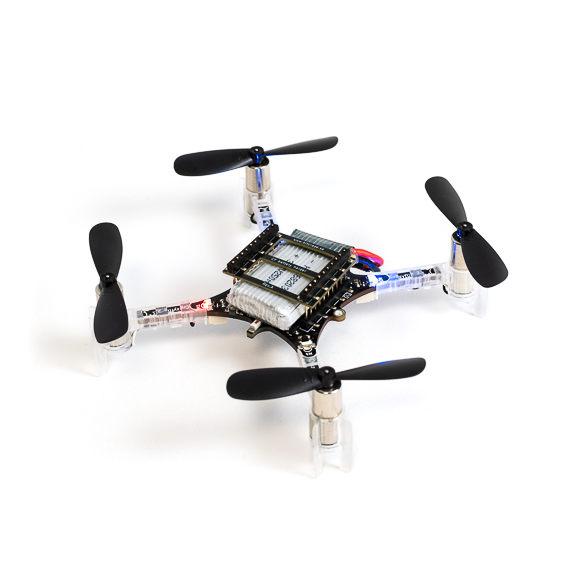
\includegraphics[trim={0 8mm 0 8mm}, clip, width=0.7\textwidth]{img/fig/fig1.1-crayzflie.jpg}
    \caption{Imagen de un Crazyflie 2.1 montado}
    \label{fig:crazyflie}
\end{figure}

Aunque los Crazyflies se pueden utilizar independientemente con un mando radiocontrol o un portátil con el conjunto del software y firmware oficial, 
el objetivo es la coordinación de movimientos entre los drones, por tanto necesitamos conocer la posición relativa o absoluta de todos los drones en tiempo real.
Por ejemplo, Bitcraze dispone de unos módulos basados en UWB (\textit{Ultra WideBand}, banda ultraancha en español) que permiten la localización de los Crazyflies en el espacio con buena precisión.
Este sistema, llamado \textit{\textbf{Loco Positioning System}} se divide en dos componentes \cite{loco_positioning_system}:

\begin{itemize}
  \item \textbf{Loco Positioning Node:} conocidos como \textit{anchors} al estar estáticos en una sala como puntos de referencia. 
  Se sitúan al menos 6 para permitir la triangulización en tres dimensiones de la posición de un Crazyflie.
  Utilizan los módulos de UWB Decawave DWM1000, ampliamente usados y conocidos módulos de UWB.
  
  \item \textbf{Loco Positioning Deck:} módulo de expansión para un Crazyflie, que le permite comunicarse con las \textit{anchors}. También utiliza los Decawave DWM1000.
\end{itemize}

\begin{figure}[h]
    \centering
    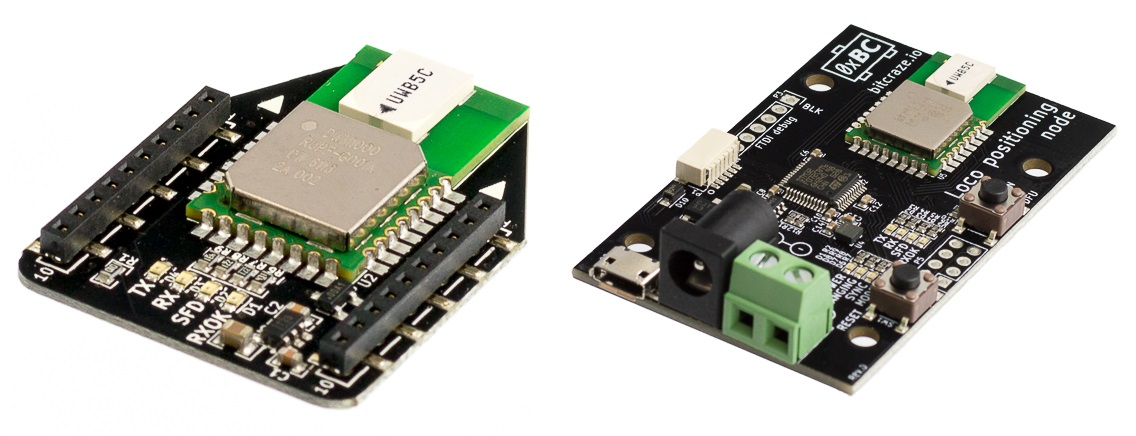
\includegraphics[clip, width=0.7\textwidth]{img/fig/fig1.2-loco-positioning-system.jpg}
    \caption{Loco Positioning Deck (izquierda). Loco Positioning Node (derecha)}
    \label{fig:loco_positioning_system}
\end{figure}

Alternativamente, tenemos otro tipo de accesorio simplificado que, 
si bien tiene menos precisión, es menos dependiente de infraestructura externa.
Se detallará en el capítulo 3, al no cobrar sentido su uso hasta ese capítulo.

%%%%%%%%%%%%%%%%%%%%%%%%%%%%%%%%%%%%%%%%%%%%%%%%%%%%%%%%%%%%%%%%%%%%%%%%%%%%%%%%%%%%%%%%%%%%%%%%%%%%%%%%%%%%%%%%%
%%%%%%%%%%%%%%%%%%%%%%%%%%%%%%%%%%%%%%%%%%%%%%%%%%%%%%%%%%%%%%%%%%%%%%%%%%%%%%%%%%%%%%%%%%%%%%%%%%%%%%%%%%%%%%%%%
%%%%%%%%%%%%%%%%%%%%%%%%%%%%%%%%%%%%%%%%%%%%%%%%%%%%%%%%%%%%%%%%%%%%%%%%%%%%%%%%%%%%%%%%%%%%%%%%%%%%%%%%%%%%%%%%%

\subsection{Software: Paparazzi UAV}

Las pruebas iniciales con el sistema serán con el conjunto del firmware oficial para los Crazyflies y el software oficial para ordenador. 
Una vez se verifique el correcto funcionamiento de cada dron, se pasará al firmware de Paparazzi para los Crazyflies. 
Junto al software de control, \textbf{Paparazzi Center} y \textbf{Paparazzi Ground Control Station} \cite{paparazzi_gcs} se completa la configuración e instalación del sistema para el control y coordinación de los UAV.

\begin{figure}[h]
    \centering
    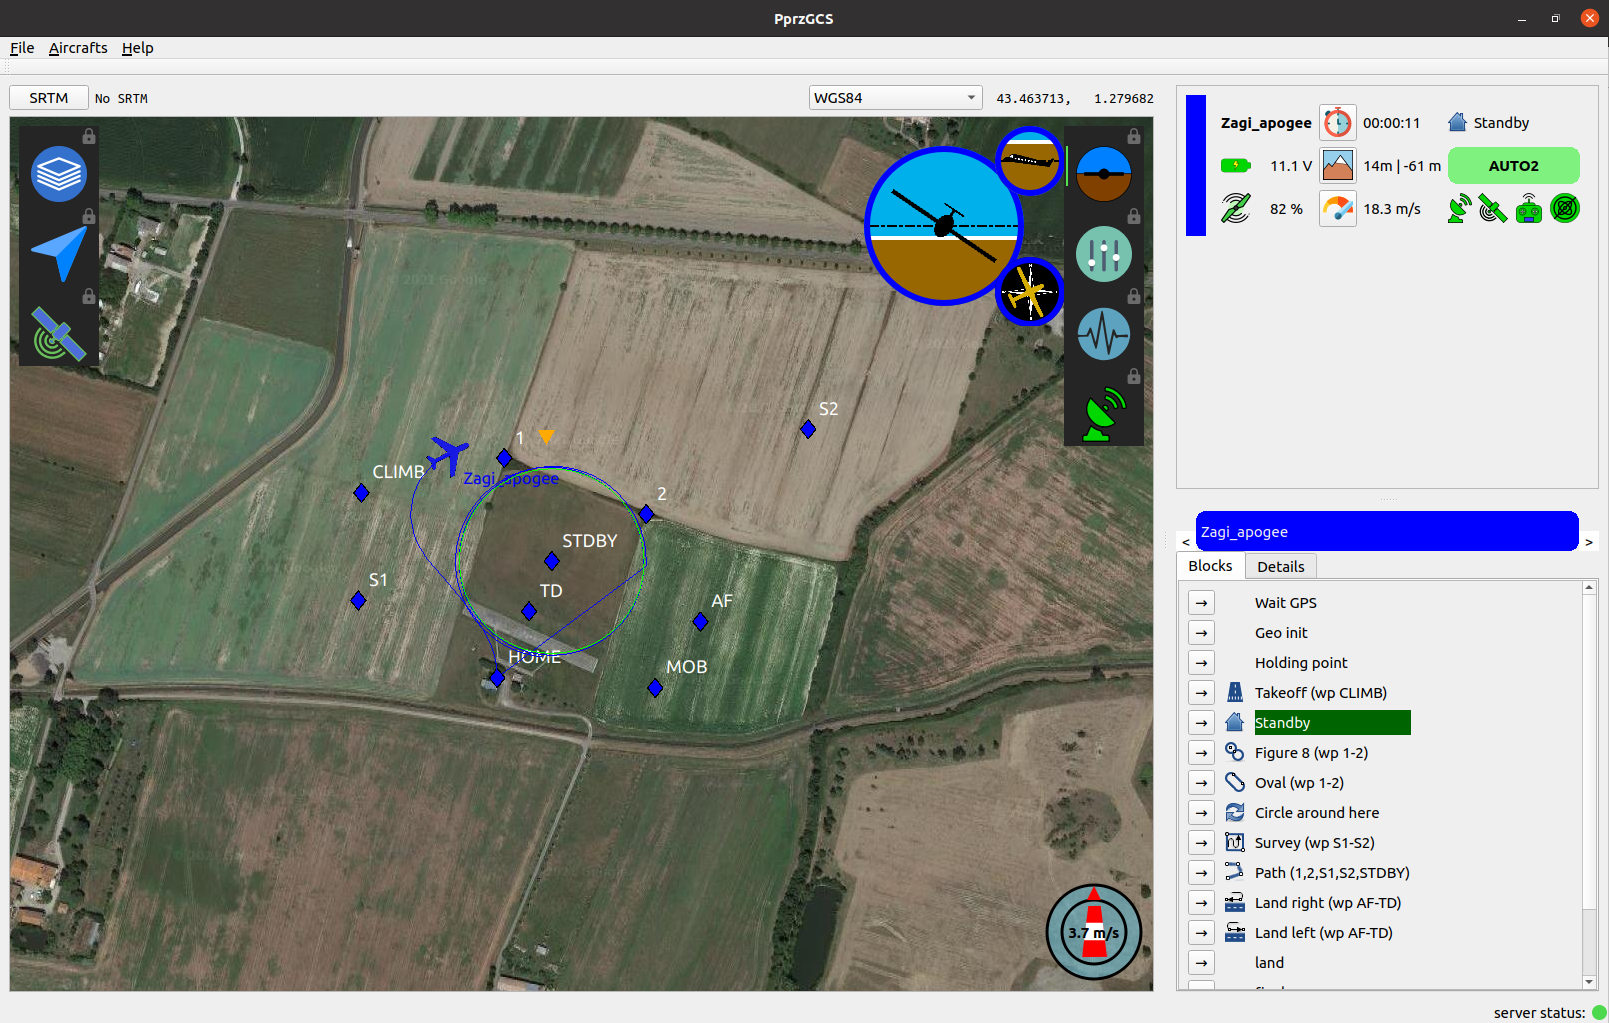
\includegraphics[width=0.88\textwidth]{img/fig/fig1.3-paparazzi-gcs.png}
    \caption{Captura de la interfaz de Paparazzi GCS}
    \label{fig:paparazzi_gcs}
\end{figure}

Para conseguir un funcionamiento completo del sistema, se necesita la implementación del posicionamiento en Paparazzi. 
Actualmente solo se dispone del firmware para los Crazyflie \cite{paparazzi_crazyflie} 
el cual únicamente permite un funcionamiento básico sin posicionamiento preciso,
al depender de exclusivamente los valores del acelerómetro.

%%%%%%%%%%%%%%%%%%%%%%%%%%%%%%%%%%%%%%%%%%%%%%%%%%%%%%%%%%%%%%%%%%%%%%%%%%%%%%%%%%%%%%%%%%%%%%%%%%%%%%%%%%%%%%%%%
%%%%%%%%%%%%%%%%%%%%%%%%%%%%%%%%%%%%%%%%%%%%%%%%%%%%%%%%%%%%%%%%%%%%%%%%%%%%%%%%%%%%%%%%%%%%%%%%%%%%%%%%%%%%%%%%%
%%%%%%%%%%%%%%%%%%%%%%%%%%%%%%%%%%%%%%%%%%%%%%%%%%%%%%%%%%%%%%%%%%%%%%%%%%%%%%%%%%%%%%%%%%%%%%%%%%%%%%%%%%%%%%%%%

\section{Objetivos}

Dada la descripción general del sistema, ya es posible entender los objetivos de este trabajo de fin de grado. Los objetivos, ordenados por capítulos y en orden cronológico de desarrollo, son los siguientes:

\begin{itemize}
    \item \textbf{OBJ-1:} introducción, objetivos, planificación y preparación general. 
    Preparación para la realización de este TFG, incluyendo la realización de este capítulo, familiarización con el ámbito, preparar la plantilla de LaTeX...
    
    \item \textbf{Capítulo 2 (OBJ-2):} preliminares. 
    Se trata de verificar que el hardware funciona de forma correcta siguiendo los pasos del fabricante, así como una breve familiarización con el control básico de un rotorcraft. 
    Tras verificación con el firmware y software oficial, se realizarán las mismas pruebas básicas con Paparazzi.

    \item \textbf{Capítulo 3 (OBJ-3):} control de un Crazyflie. 
    Se conseguirá un control mínimo y estabilizado de un solo Crazyflie (\textit{hovering}).
    Se usará un algoritmo de seguimiento de trayectorias que será implementado en el firmware de Paparazzi.

    \item \textbf{Capítulo 4 (OBJ-4):} coordinación entre Crazyflies. 
    Se añade al objetivo 3 la capacidad de coordinar dos o más drones para seguir trayectorias de forma coordinada (formaciones).

    \item \textbf{Capítulo 5 (OBJ-5):} terminamos este TFG con las conclusiones extraídas, resultados obtenidos, análisis de la planificación y objetivos cumplidos.

    \item \textbf{OBJ-6:} Revisión y mejora general previo de este trabajo. Afecta a todos los objetivos.
    Se añade la realización completa de la presentación en diapositivas y la finalización de esta memoria.
\end{itemize}

Resumidamente, se trata de conseguir que los Crazyflies puedan seguir trayectorias de forma coordinada utilizando el conjunto de firmware y software \textit{open source} de Paparazzi UAV.

%%%%%%%%%%%%%%%%%%%%%%%%%%%%%%%%%%%%%%%%%%%%%%%%%%%%%%%%%%%%%%%%%%%%%%%%%%%%%%%%%%%%%%%%%%%%%%%%%%%%%%%%%%%%%%%%%
%%%%%%%%%%%%%%%%%%%%%%%%%%%%%%%%%%%%%%%%%%%%%%%%%%%%%%%%%%%%%%%%%%%%%%%%%%%%%%%%%%%%%%%%%%%%%%%%%%%%%%%%%%%%%%%%%
%%%%%%%%%%%%%%%%%%%%%%%%%%%%%%%%%%%%%%%%%%%%%%%%%%%%%%%%%%%%%%%%%%%%%%%%%%%%%%%%%%%%%%%%%%%%%%%%%%%%%%%%%%%%%%%%%

\section{Planificación}

Para cumplir los objetivos provistos se ha realizado la siguiente planificación:

\begin{figure}[h]
    \centering
    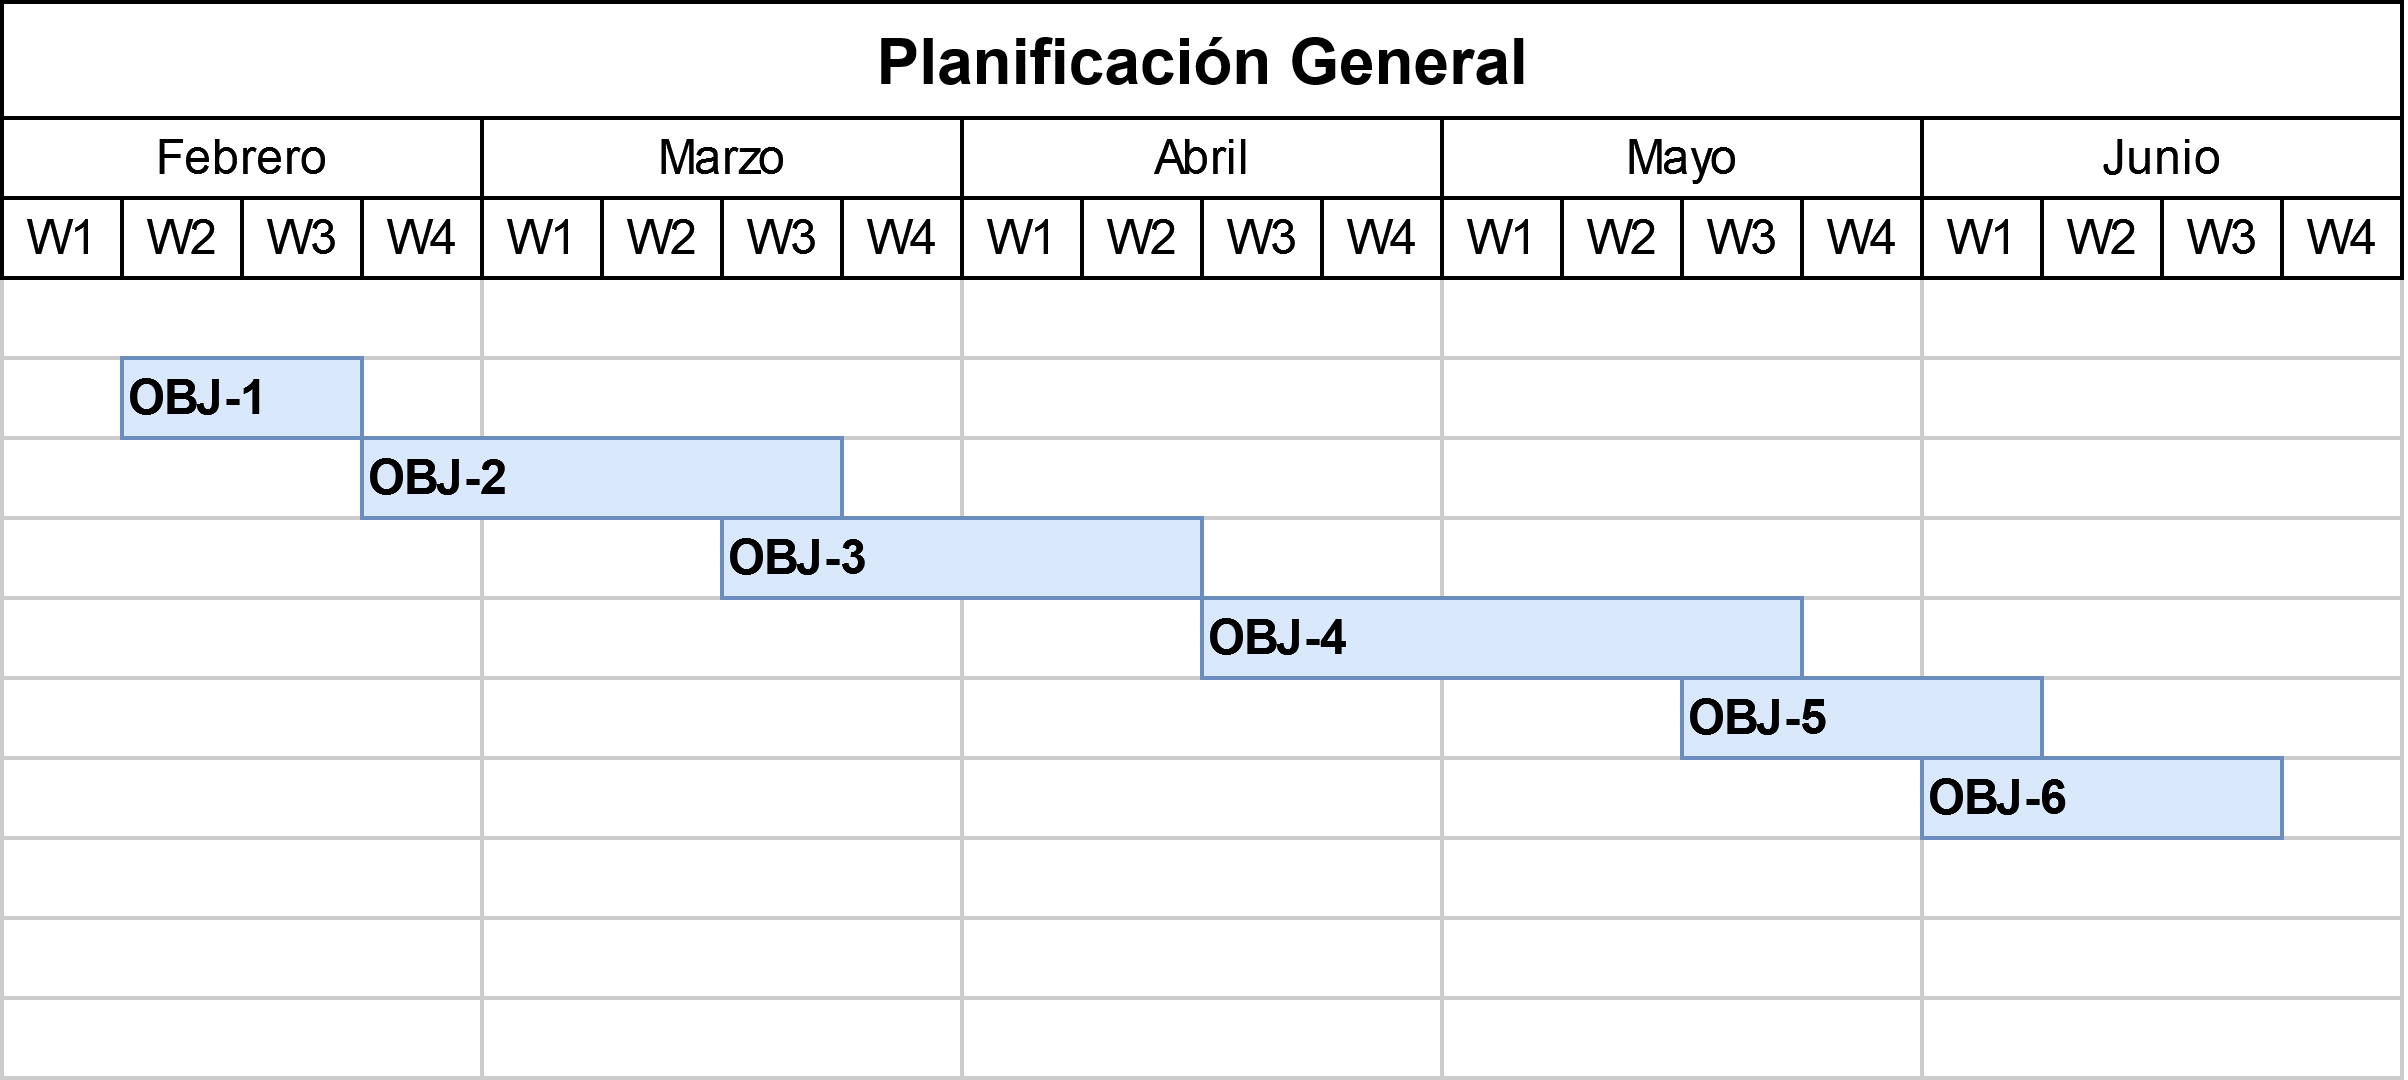
\includegraphics[width=0.99\textwidth]{img/fig/fig1.4-gantt.png}
    \caption{Planificación de este trabajo}
    \label{fig:gantt}
\end{figure}

Por supuesto, esta planificación es aproximada y flexible hasta cierto punto.
Debido a la naturaleza de este trabajo, es difícil preveer con exactitud el correcto desarrollo de la planificación,
al requerir un estudio constante de una tecnología en desarrollo con multitud de opciones, así como la dependencia de un proyecto de ámbito \textit{open source},
en constante evolución con los posibles problemas y contratiempos que ello puede ocasionar, por ejemplo, las actualizaciones de este.

En el último capítulo, se hará una comparación entre esta planificación y el resultado final de esta, 
con objetivo de entender que ha pasado durante el desarrollo de este trabajo
y si el desarrollo ha ido como fue planeado. 
    \chapter{Preliminares}

Tras una breve introducción a los dispositivos que se usarán para el desarrollo de esta obra, procederemos a las primeros pasos necesarios para la configuración y control de los drones.

En adelante, se detallan los procedimientos para lo que es conocido como \textit{Maiden Flight}, 
el primer vuelo de cualquier tipo de vehículo aeronáutico o aeroespacial. 
Posteriormente, tras las pruebas con el firmware y software oficiales, se realizarán las mismas pruebas con el firmware del proyecto Paparazzi UAV.

%%%%%%%%%%%%%%%%%%%%%%%%%%%%%%%%%%%%%%%%%%%%%%%%%%%%%%%%%%%%%%%%%%%%%%%%%%%%%%%%%%%%%%%%%%%%%%%%%%%%%%%%%%%%%%%%%
%%%%%%%%%%%%%%%%%%%%%%%%%%%%%%%%%%%%%%%%%%%%%%%%%%%%%%%%%%%%%%%%%%%%%%%%%%%%%%%%%%%%%%%%%%%%%%%%%%%%%%%%%%%%%%%%%
%%%%%%%%%%%%%%%%%%%%%%%%%%%%%%%%%%%%%%%%%%%%%%%%%%%%%%%%%%%%%%%%%%%%%%%%%%%%%%%%%%%%%%%%%%%%%%%%%%%%%%%%%%%%%%%%%

\section{Montaje de los drones}

Cada Crazyflie 2.1 necesita de montaje manual. Para ello, se ha seguido la guía oficial del fabricante \cite{crazyflie_assembly_and_quickstart}.
Los componentes de un Crazyflie necesarios para el montaje son los siguientes:

\begin{table}[h]
\centering
\begin{tabular}{l|c}
    \multicolumn{1}{c|}{\textbf{Componente}} & \textbf{Cantidad} \\ \hline
    Crazyflie 2.1 Board             & 1        \\
    Hélices tipo CW                 & 2        \\
    Hélices tipo CCW                & 2        \\
    Anclajes para motores           & 4        \\
    Motores DC                      & 4        \\
    Batería LiPo                    & 1        \\
    Anclaje para batería            & 1        \\
    Pines de expansión              & 1       
\end{tabular}
    \caption{Componentes de un Crazyflie 2.1}
    \label{tab:componentes_crazyflie}
\end{table}

Además, podemos ver en esta figura los componentes de un Crazyflie previo a su montaje:

\begin{figure}[h]
    \centering
    \includegraphics[width=0.88\textwidth]{img/fig/fig2.1-crazyflie-disassembled.jpg}
    \caption{Componentes de un Crazyflie 2.1}
    \label{fig:crazyflie_disassembled}
\end{figure}

El procedimiento de montaje, a efectos simplificados, es el siguiente. Se sigue, como bien se ha indicado previamente, 
la guía oficial \cite{crazyflie_assembly_and_quickstart}:

\begin{itemize}
    \item Montaje de los motores en cada anclaje para estos.
    \item Insertar los anclajes en el Crazyflie 2.1 y conectar los motores eléctricamente a este.
    \item Añadir las hélices a los motores, diferenciando las CW (\textit{ClockWise}) de las CCW (\textit{CounterClockWise}).
    \item Montar los pines de expansión y la batería.
    \item Anclar la batería utilizando el anclaje de la batería, que se conecta a los pines de expansión.
\end{itemize}

%%%%%%%%%%%%%%%%%%%%%%%%%%%%%%%%%%%%%%%%%%%%%%%%%%%%%%%%%%%%%%%%%%%%%%%%%%%%%%%%%%%%%%%%%%%%%%%%%%%%%%%%%%%%%%%%%
%%%%%%%%%%%%%%%%%%%%%%%%%%%%%%%%%%%%%%%%%%%%%%%%%%%%%%%%%%%%%%%%%%%%%%%%%%%%%%%%%%%%%%%%%%%%%%%%%%%%%%%%%%%%%%%%%
%%%%%%%%%%%%%%%%%%%%%%%%%%%%%%%%%%%%%%%%%%%%%%%%%%%%%%%%%%%%%%%%%%%%%%%%%%%%%%%%%%%%%%%%%%%%%%%%%%%%%%%%%%%%%%%%%

\section{Pruebas con software oficial}

Con un Crazyflie montado, podemos proceder a las pruebas iniciales con el conjunto de software y firmware oficial.
Desde la guía oficial de montaje se recomienda utilizar la máquina virtual preconfigurada por Bitcraze para conseguir
volar el rotorcraft lo antes posible \cite{bitcraze_vm}. En esta máquina virtual se incluye los programas para el control,
código fuente y otros recursos software de utilidad para el desarrollo con Crazyflies.

%%%%%%%%%%%%%%%%%%%%%%%%%%%%%%%%%%%%%%%%%%%%%%%%%%%%%%%%%%%%%%%%%%%%%%%%%%%%%%%%%%%%%%%%%%%%%%%%%%%%%%%%%%%%%%%%%
%%%%%%%%%%%%%%%%%%%%%%%%%%%%%%%%%%%%%%%%%%%%%%%%%%%%%%%%%%%%%%%%%%%%%%%%%%%%%%%%%%%%%%%%%%%%%%%%%%%%%%%%%%%%%%%%%
%%%%%%%%%%%%%%%%%%%%%%%%%%%%%%%%%%%%%%%%%%%%%%%%%%%%%%%%%%%%%%%%%%%%%%%%%%%%%%%%%%%%%%%%%%%%%%%%%%%%%%%%%%%%%%%%%

\subsection{Preparación}

Previo a la conexión con un Crazyflie, debemos de cargar el firmware al Crazyradio 2.0, el módulo USB que nos permite controlar 
remotamente un Crazyflie y recibir telemetría de este. Para ello, se sigue la guía oficial del fabricante \cite{crazyradio_setup}.

\begin{figure}[h]
    \centering
    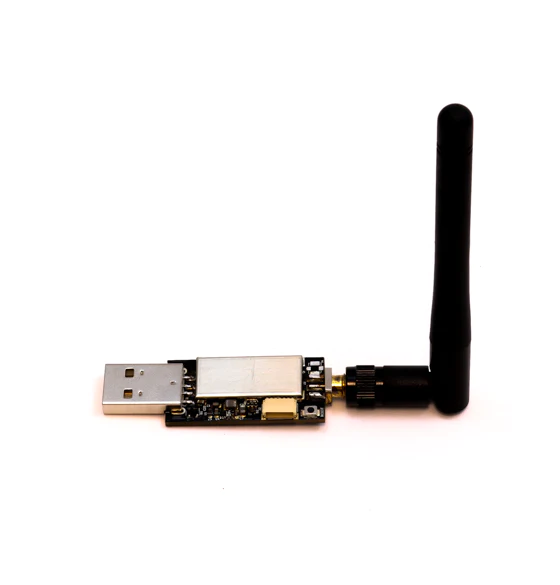
\includegraphics[width=0.65\textwidth]{img/fig/fig2.2-crazyradio.png}
    \caption{Crazyradio 2.0}
    \label{fig:crazyradio}
\end{figure}

Con ello, ya podemos conectarnos a un Crazyflie desde el software de control Crazyflie Client, no obstante, 
se recomienda actualizar el firmware del Crazyflie 2.1 previamente utilizando Crazyflie Client. 
Se sigue la guía oficial de actualización de firmware \cite{crazyflie_firmware_upgrade}.

%%%%%%%%%%%%%%%%%%%%%%%%%%%%%%%%%%%%%%%%%%%%%%%%%%%%%%%%%%%%%%%%%%%%%%%%%%%%%%%%%%%%%%%%%%%%%%%%%%%%%%%%%%%%%%%%%
%%%%%%%%%%%%%%%%%%%%%%%%%%%%%%%%%%%%%%%%%%%%%%%%%%%%%%%%%%%%%%%%%%%%%%%%%%%%%%%%%%%%%%%%%%%%%%%%%%%%%%%%%%%%%%%%%
%%%%%%%%%%%%%%%%%%%%%%%%%%%%%%%%%%%%%%%%%%%%%%%%%%%%%%%%%%%%%%%%%%%%%%%%%%%%%%%%%%%%%%%%%%%%%%%%%%%%%%%%%%%%%%%%%

\subsection{Control básico con Crazyflie Client}

El último paso previo a cambiar al proyecto Paparazzi consiste en familiarizarse con el control básico de un solo Crazyflie 
mediante el software oficial. De esta forma se confirma también el correcto funcionamiento de cada dron, asegurando que no es fallo
de firmware/software no oficiales (Paparazzi, en este caso). Aquí podemos ver la interfaz de Crazyflie Client:

\begin{figure}[h]
    \centering
    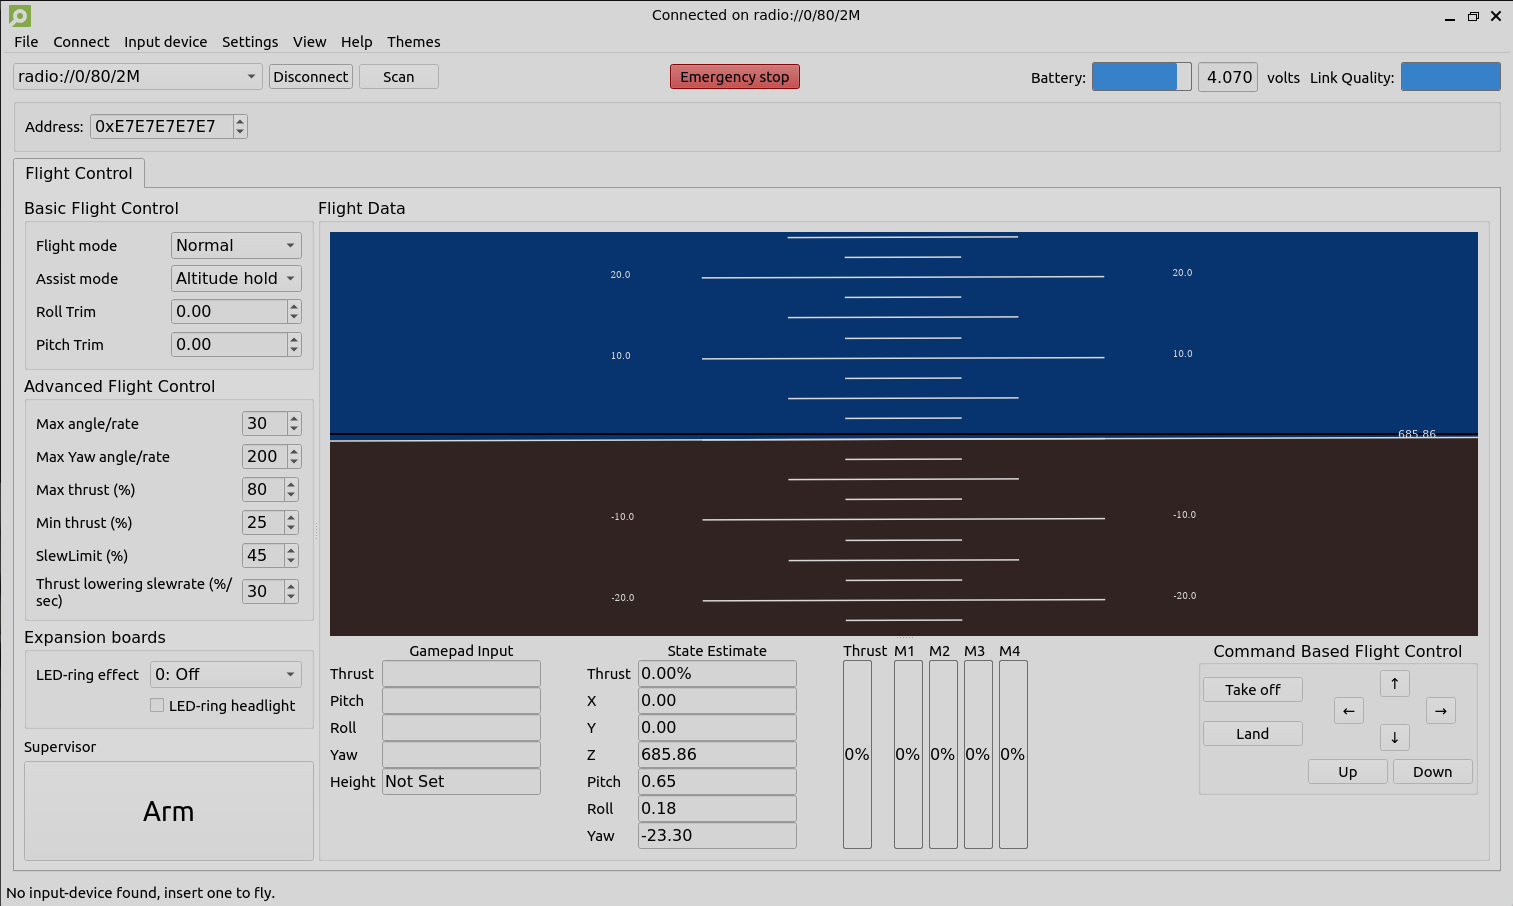
\includegraphics[width=0.96\textwidth]{img/fig/fig2.3-crazyflie-client.png}
    \caption{Interfaz de Crazyflie Client}
    \label{fig:crazyflie-client}
\end{figure}

\subsection{Variables de control en Crazyflie Client}

Previo a continuar con el desarrollo de este trabajo, es importante entender las variables básicas que definen como se desarrolla el vuelo de un rotorcraft.
Aunque existen más, introduciremos aquí todas las variables que Crazyflie Client nos permite saber de un Crazyflie. 

En la siguiente tabla se detallan las variables, así como la unidad del Sistema Internacional que se utiliza. 
Se indican unidades alternativas entre paréntesis, muy utilizadas en otras situaciones o programas. 

\begin{table}[h]
\centering
\begin{tabular}{c|c|c}
    \textbf{Variable} & \textbf{Descripción} & \textbf{Unidad} \\ \hline
    Roll     & Rotación sobre el eje X   & Grados (Radianes) \\
    Pitch    & Rotación sobre el eje Y   & Grados (Radianes) \\
    Yaw      & Rotación sobre el eje Z   & Grados (Radianes) \\
    X        & Posición en el eje X      & m                 \\
    Y        & Posición en el eje Y      & m                 \\
    Z        & Posición en el eje Z      & m                 \\
    Height   & Altura respecto al suelo  & m                 \\
    Thrust   & Empuje de los motores     & \%                \\
    Battery  & Nivel restante de batería & V (\%)            
\end{tabular}
    \caption{Variables de control de un Crazyflie en Crazyflie Client}
    \label{tab:crazyflie_client_vars}
\end{table}

Cabe destacar las variables \textbf{roll, pitch y yaw} que indican la rotación de un objeto respecto a alguno de sus ejes.
Son variables muy usadas en el ámbito de control de vehículos aéreos y aeroespaciales. La siguiente imagen describe de forma 
gráfica cada una de estas variables.

\begin{figure}[h]
    \centering
    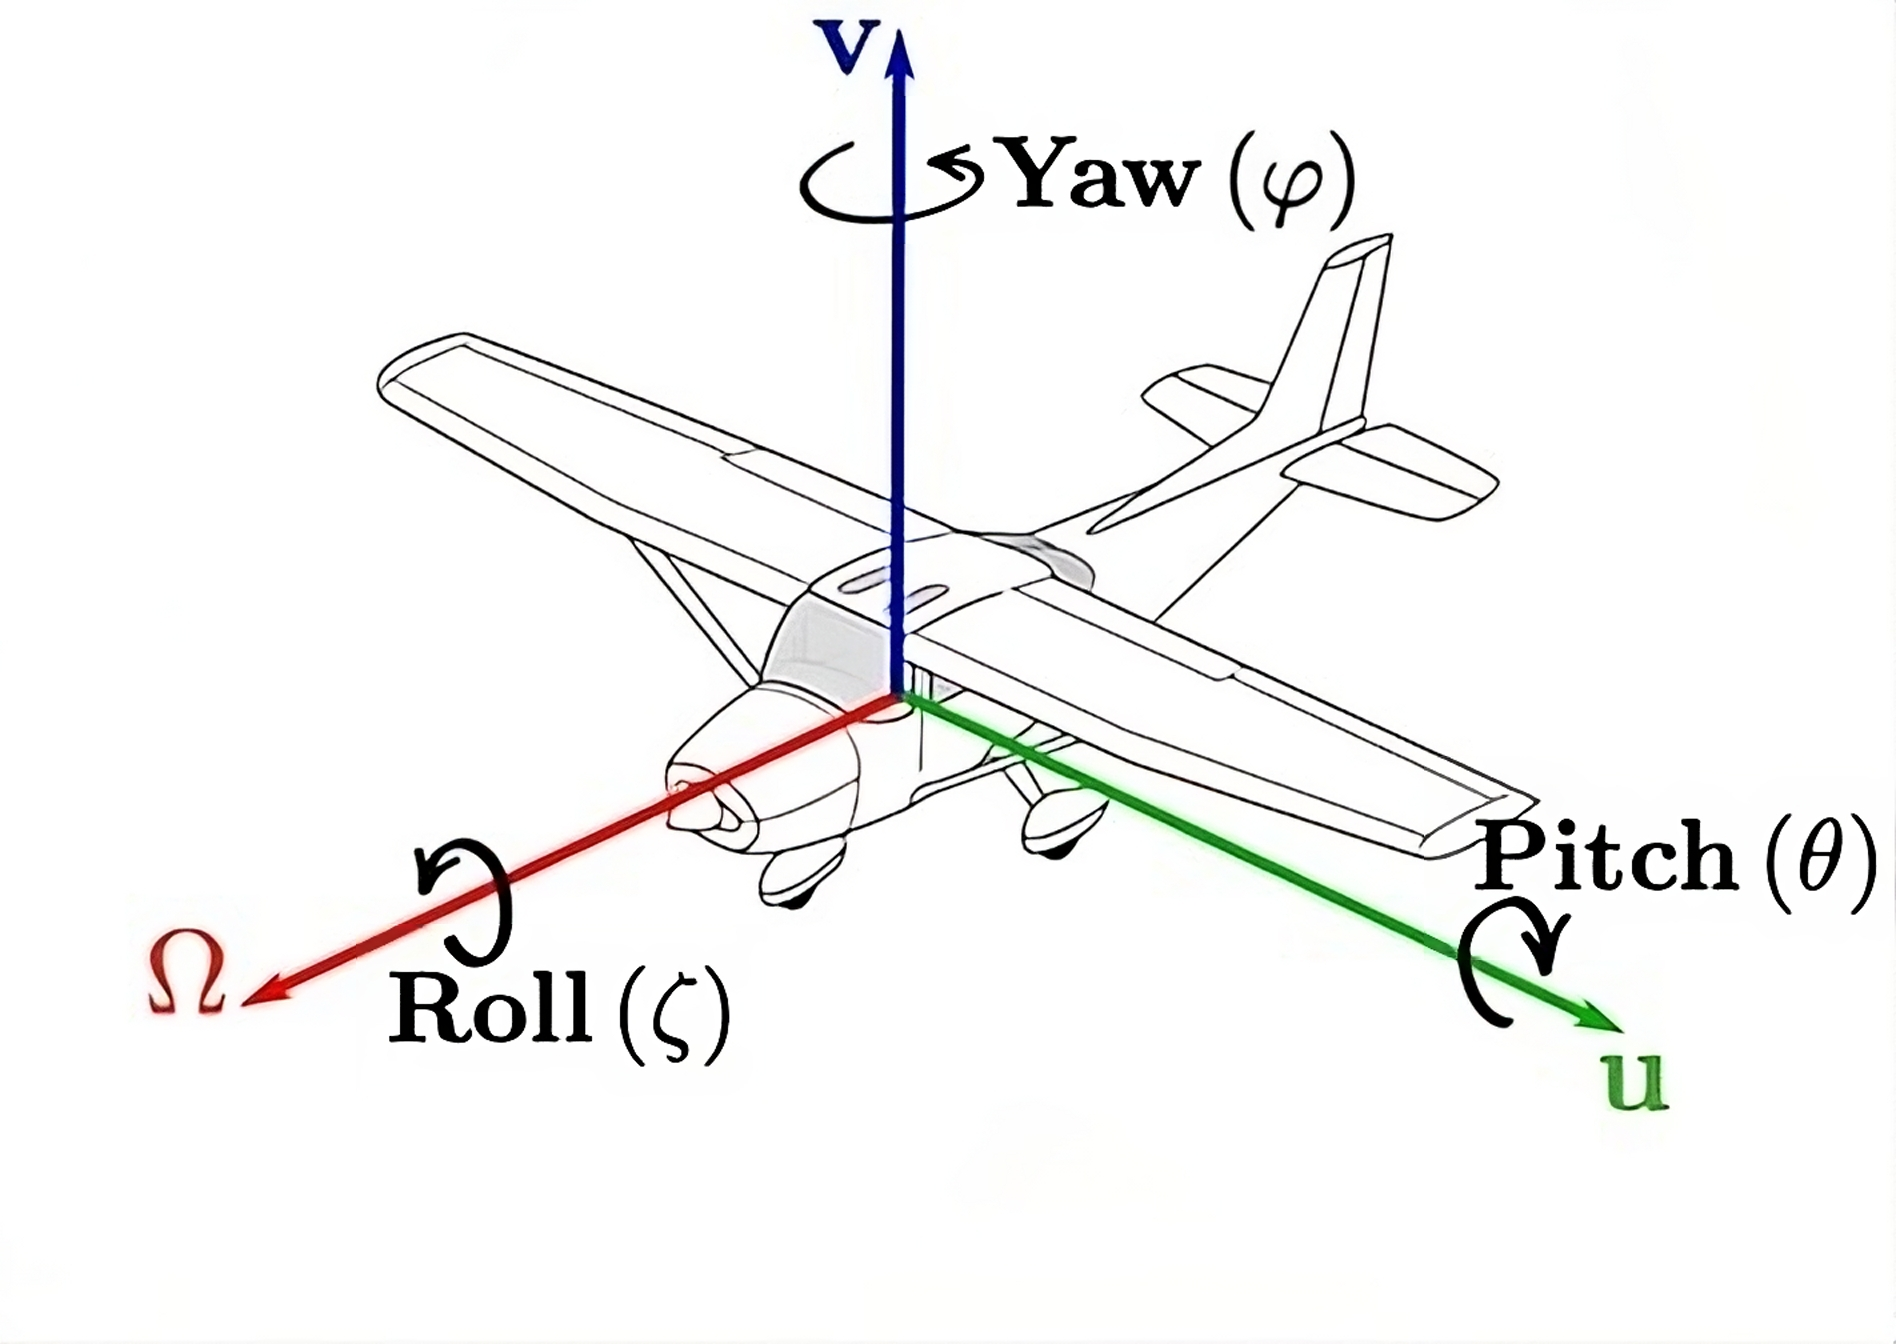
\includegraphics[width=0.9\textwidth]{img/fig/fig2.4-rotational-axes.jpeg}
    \caption{Ejes de rotación de un vehículo aéreo}
    \label{fig:rotational-axes}
\end{figure}

%%%%%%%%%%%%%%%%%%%%%%%%%%%%%%%%%%%%%%%%%%%%%%%%%%%%%%%%%%%%%%%%%%%%%%%%%%%%%%%%%%%%%%%%%%%%%%%%%%%%%%%%%%%%%%%%%
%%%%%%%%%%%%%%%%%%%%%%%%%%%%%%%%%%%%%%%%%%%%%%%%%%%%%%%%%%%%%%%%%%%%%%%%%%%%%%%%%%%%%%%%%%%%%%%%%%%%%%%%%%%%%%%%%
%%%%%%%%%%%%%%%%%%%%%%%%%%%%%%%%%%%%%%%%%%%%%%%%%%%%%%%%%%%%%%%%%%%%%%%%%%%%%%%%%%%%%%%%%%%%%%%%%%%%%%%%%%%%%%%%%

\section{Pruebas con Paparazzi UAV}

Realizadas el montaje y pruebas iniciales, el siguiente paso consiste en la familiarización con el ecosistema Paparazzi.
Se instalará Paparazzi Center y acto seguido se realizará una breve simulación de vuelo en Paparazzi GCS. 
Tras ello, se cargará el firmware de Paparazzi para un Crazyflie y se realizará la primera prueba real.

%%%%%%%%%%%%%%%%%%%%%%%%%%%%%%%%%%%%%%%%%%%%%%%%%%%%%%%%%%%%%%%%%%%%%%%%%%%%%%%%%%%%%%%%%%%%%%%%%%%%%%%%%%%%%%%%%
%%%%%%%%%%%%%%%%%%%%%%%%%%%%%%%%%%%%%%%%%%%%%%%%%%%%%%%%%%%%%%%%%%%%%%%%%%%%%%%%%%%%%%%%%%%%%%%%%%%%%%%%%%%%%%%%%
%%%%%%%%%%%%%%%%%%%%%%%%%%%%%%%%%%%%%%%%%%%%%%%%%%%%%%%%%%%%%%%%%%%%%%%%%%%%%%%%%%%%%%%%%%%%%%%%%%%%%%%%%%%%%%%%%

\subsection{Paparazzi Center}

La instalación de Paparazzi Center se ha realizado siguiendo la guía oficial \cite{paparazzi_center_install}, con leves modificaciones para adaptarlo a Debian 12 (véase \autoref{appendix:debian_install}). En la siguiente imagen podemos ver la interfaz de Paparazzi Center en Debian 12 con KDE Plasma 5: 

\begin{figure}[h]
    \centering
    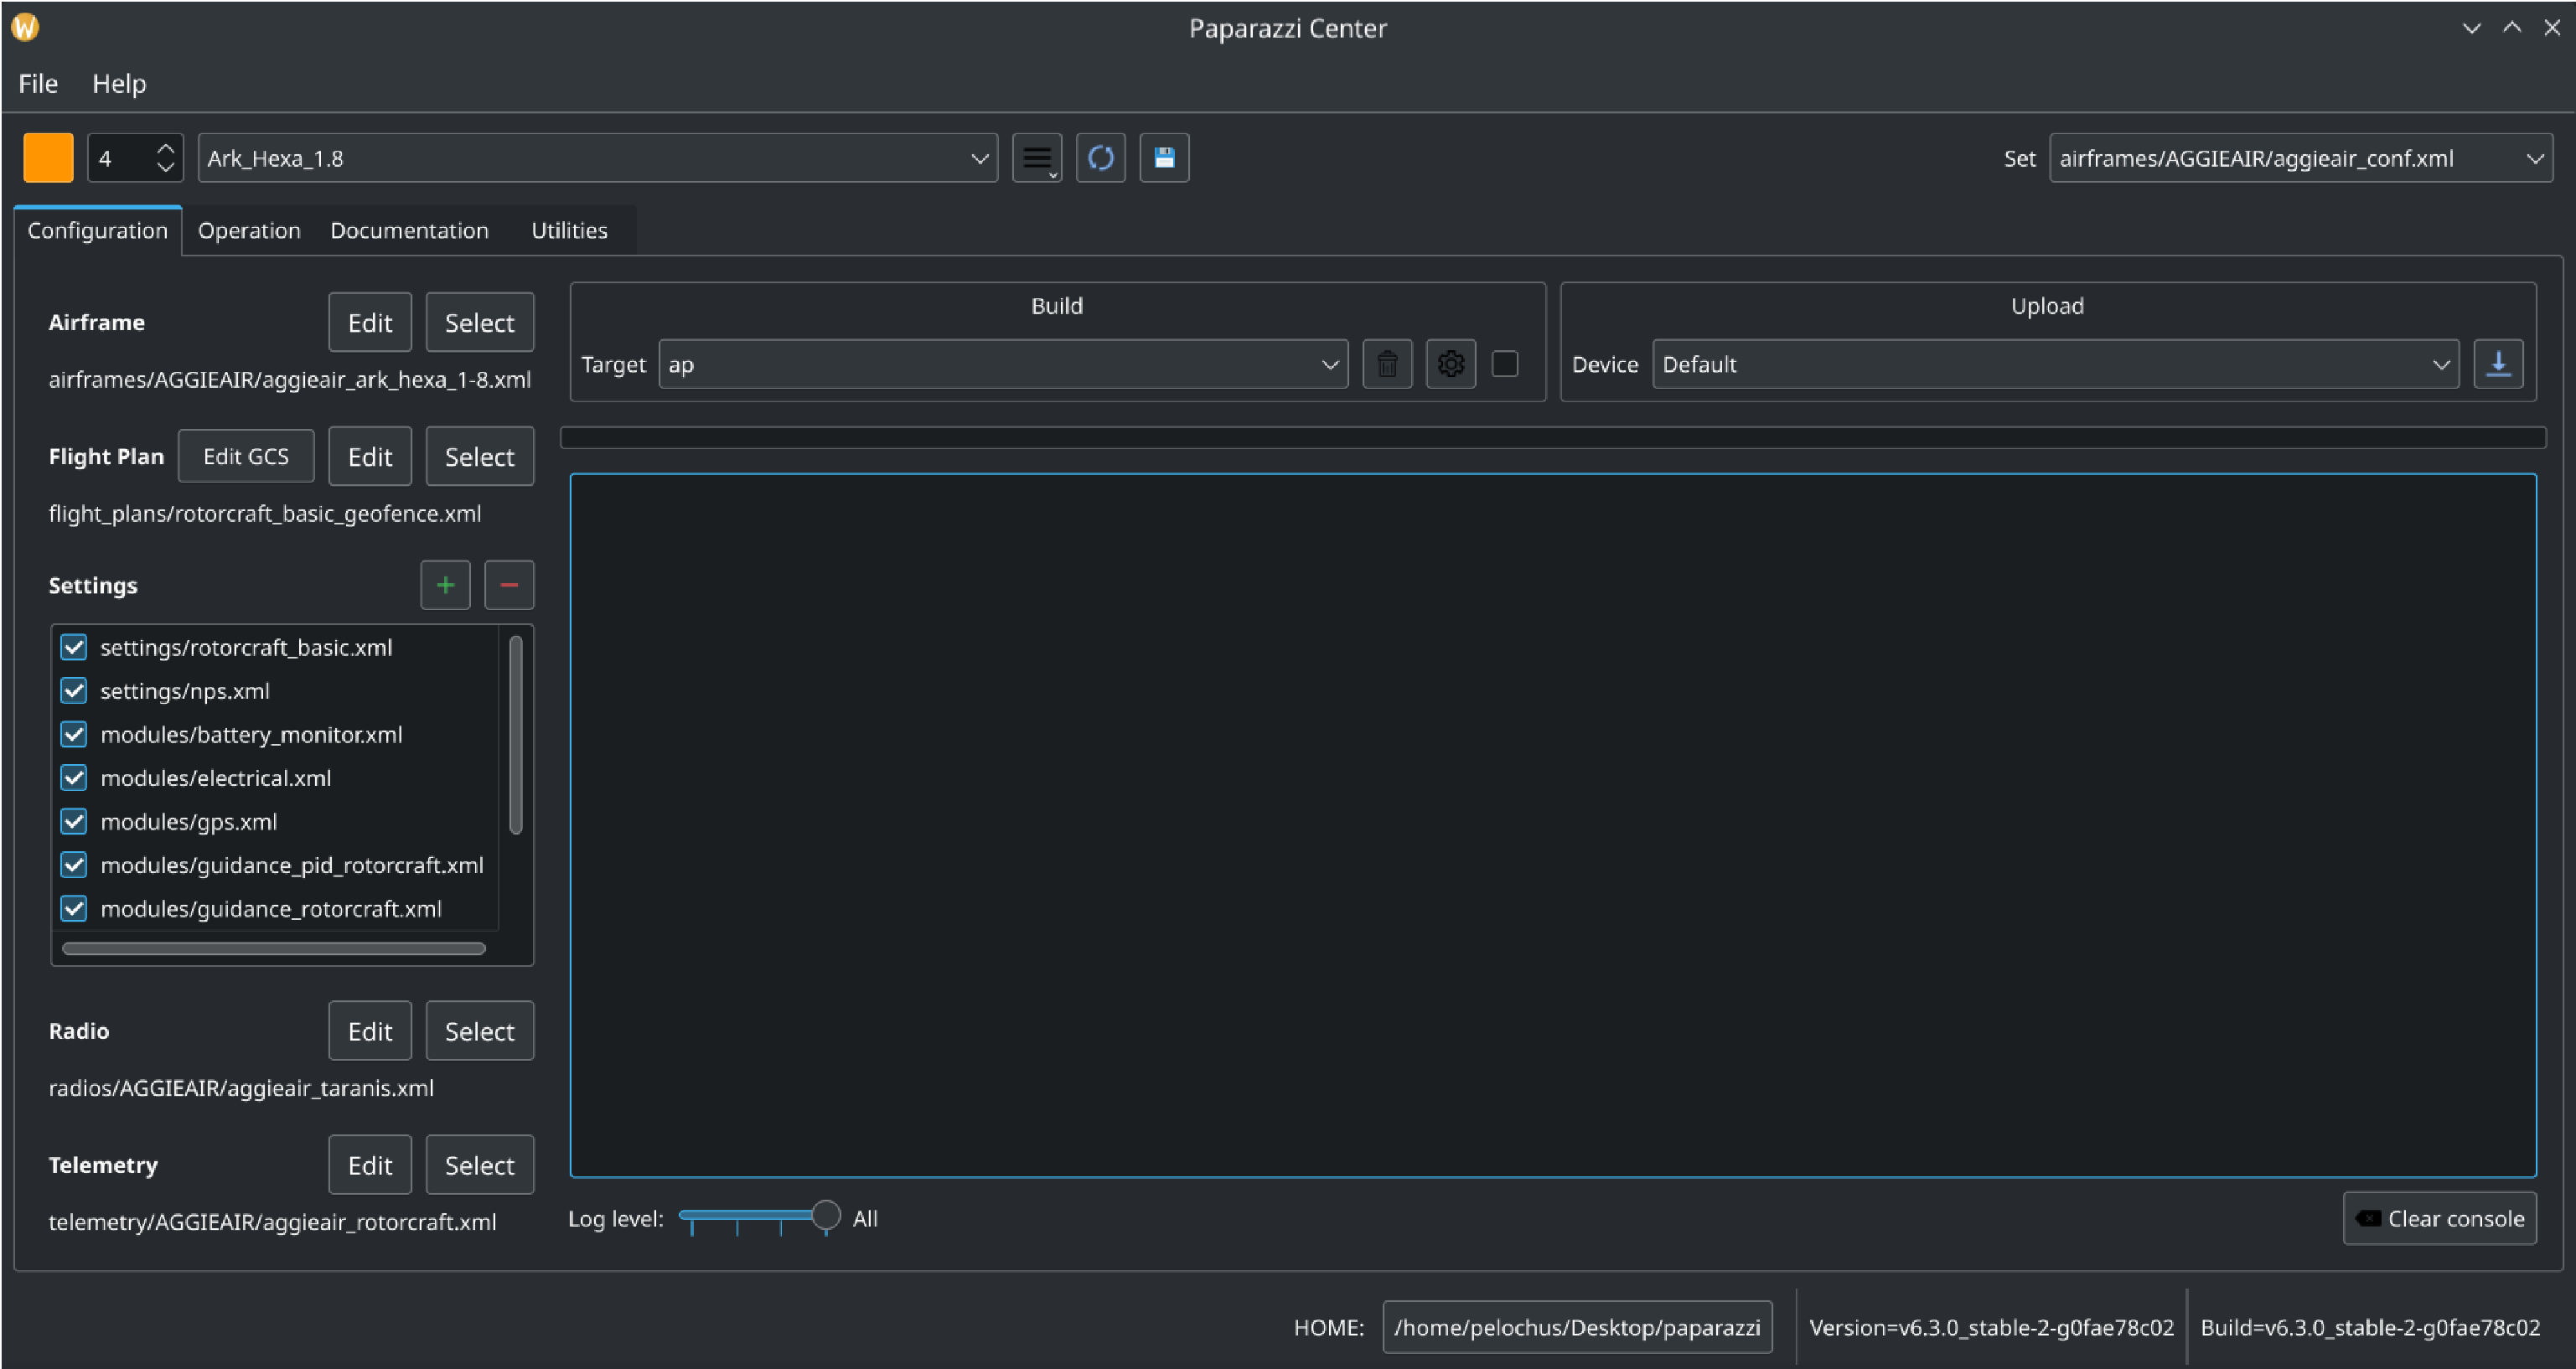
\includegraphics[width=0.92\textwidth]{img/fig/fig2.5-paparazzi-center.png}
    \caption{Captura de Paparazzi Center bajo Debian 12 con KDE}
    \label{fig:paparazzi-center}
\end{figure}

Desde Paparazzi Center se puede realizar simulaciones, planes de vuelo, observar mensajes de la consola, 
seleccionar el UAV deseado y un largo etcétera de posibilidades.
Se utilizará principalmente los paneles de operación de vuelo, simulación de vuelo, ajustes y consola para depuración.

%%%%%%%%%%%%%%%%%%%%%%%%%%%%%%%%%%%%%%%%%%%%%%%%%%%%%%%%%%%%%%%%%%%%%%%%%%%%%%%%%%%%%%%%%%%%%%%%%%%%%%%%%%%%%%%%%
%%%%%%%%%%%%%%%%%%%%%%%%%%%%%%%%%%%%%%%%%%%%%%%%%%%%%%%%%%%%%%%%%%%%%%%%%%%%%%%%%%%%%%%%%%%%%%%%%%%%%%%%%%%%%%%%%
%%%%%%%%%%%%%%%%%%%%%%%%%%%%%%%%%%%%%%%%%%%%%%%%%%%%%%%%%%%%%%%%%%%%%%%%%%%%%%%%%%%%%%%%%%%%%%%%%%%%%%%%%%%%%%%%%

\subsection{Simulaciones en Paparazzi Center}

Siguiendo la documentación de Paparazzi  podemos realizar la primera simulación \cite{paparazzi_first_simulation}. 
Seguir los pasos resulta en la apertura de Paparazzi GCS.

\begin{figure}[h]
    \centering
    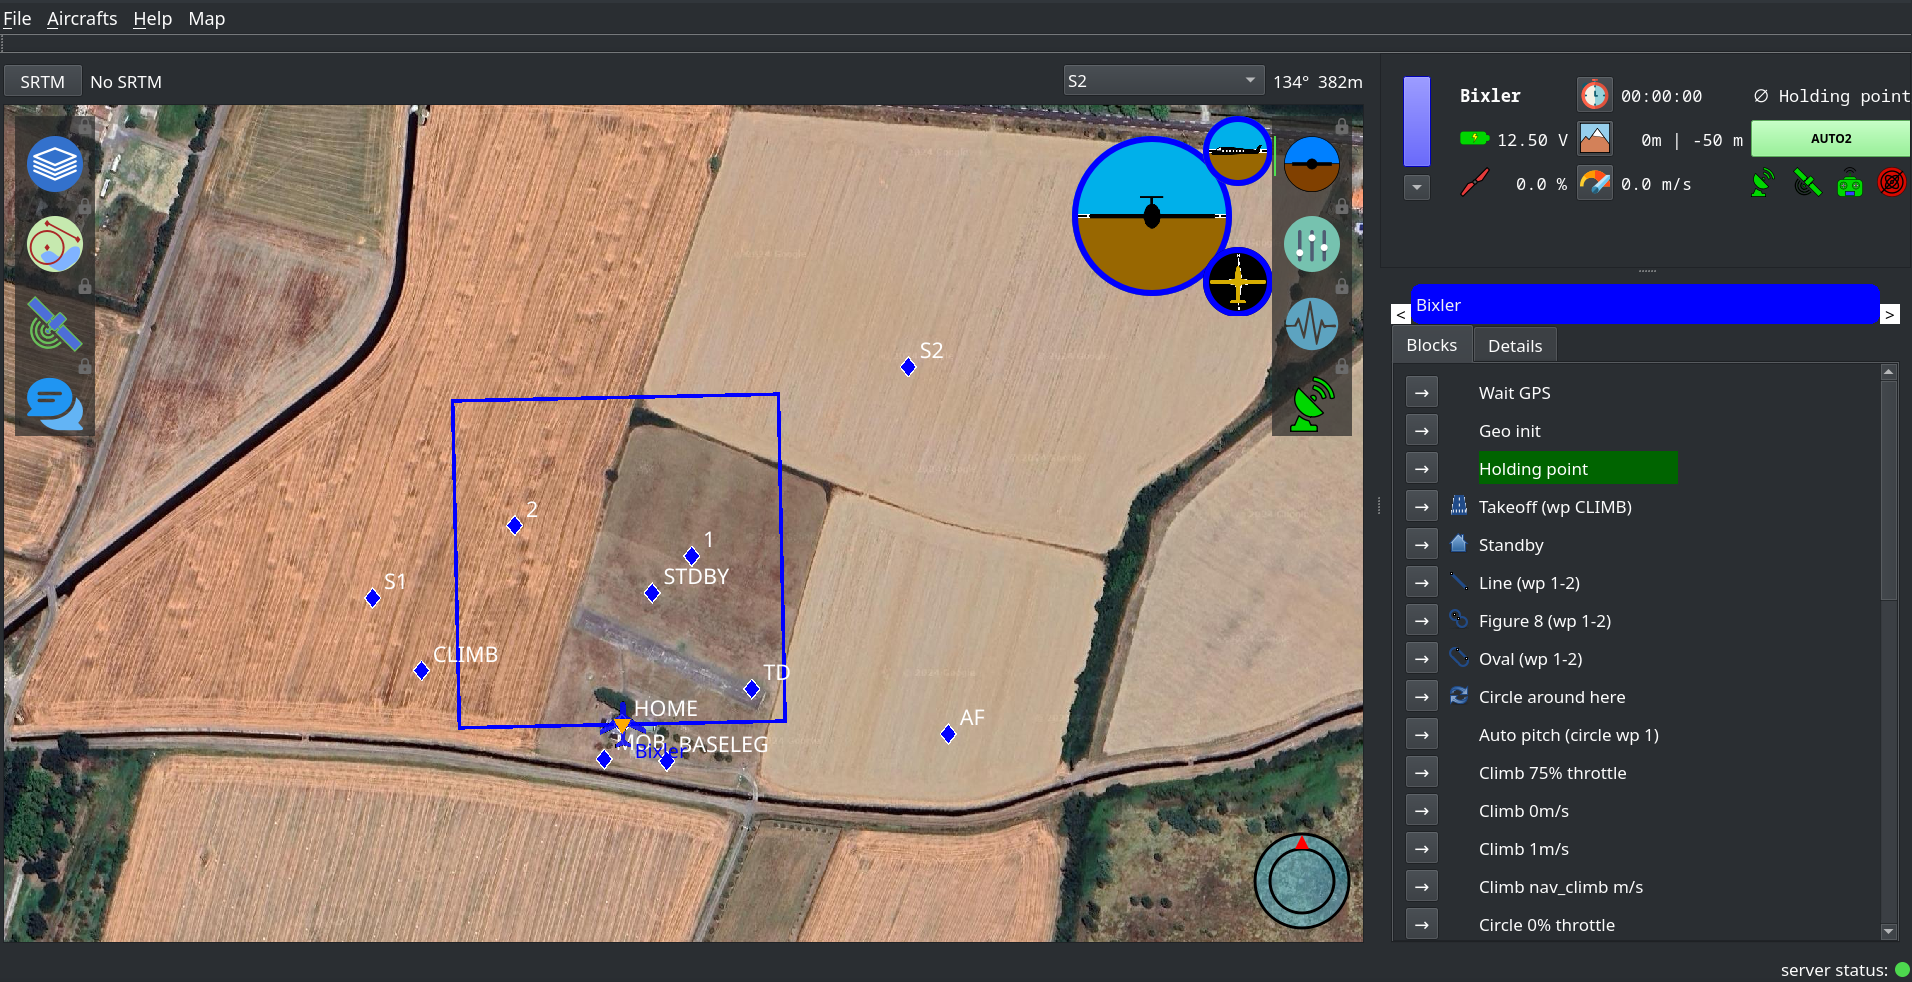
\includegraphics[width=0.9\textwidth]{img/fig/fig2.6-paparazzi-gcs-first-sim.png}
    \caption{Paparazzi GCS ejecutando la simulación por defecto}
    \label{fig:paparazzi-first-simulation}
\end{figure}

Desde Paparazzi GCS tenemos un sinfín de posibilidades más que desde Crazyflie Client. Cabe destacar, por ejemplo,
la capacidad realizar simulaciones en una zona del planeta cualquiera. Esto se puede aplicar a las misiones de 
vuelo reales, es decir, mediante GPS indicar en que zona estamos volando. 

Por otro lado, tenemos la capacidad de observar una gran cantidad de variables, incluso personalizar cuales 
queremos ver y cuales no, controles y órdenes de todo tipo, capacidad para elegir \textit{waypoints} etc...

%%%%%%%%%%%%%%%%%%%%%%%%%%%%%%%%%%%%%%%%%%%%%%%%%%%%%%%%%%%%%%%%%%%%%%%%%%%%%%%%%%%%%%%%%%%%%%%%%%%%%%%%%%%%%%%%%
%%%%%%%%%%%%%%%%%%%%%%%%%%%%%%%%%%%%%%%%%%%%%%%%%%%%%%%%%%%%%%%%%%%%%%%%%%%%%%%%%%%%%%%%%%%%%%%%%%%%%%%%%%%%%%%%%
%%%%%%%%%%%%%%%%%%%%%%%%%%%%%%%%%%%%%%%%%%%%%%%%%%%%%%%%%%%%%%%%%%%%%%%%%%%%%%%%%%%%%%%%%%%%%%%%%%%%%%%%%%%%%%%%%

\subsection{Firmware de Paparazzi para Crazyflie 2.1}

\begin{figure}[h]
    \centering
    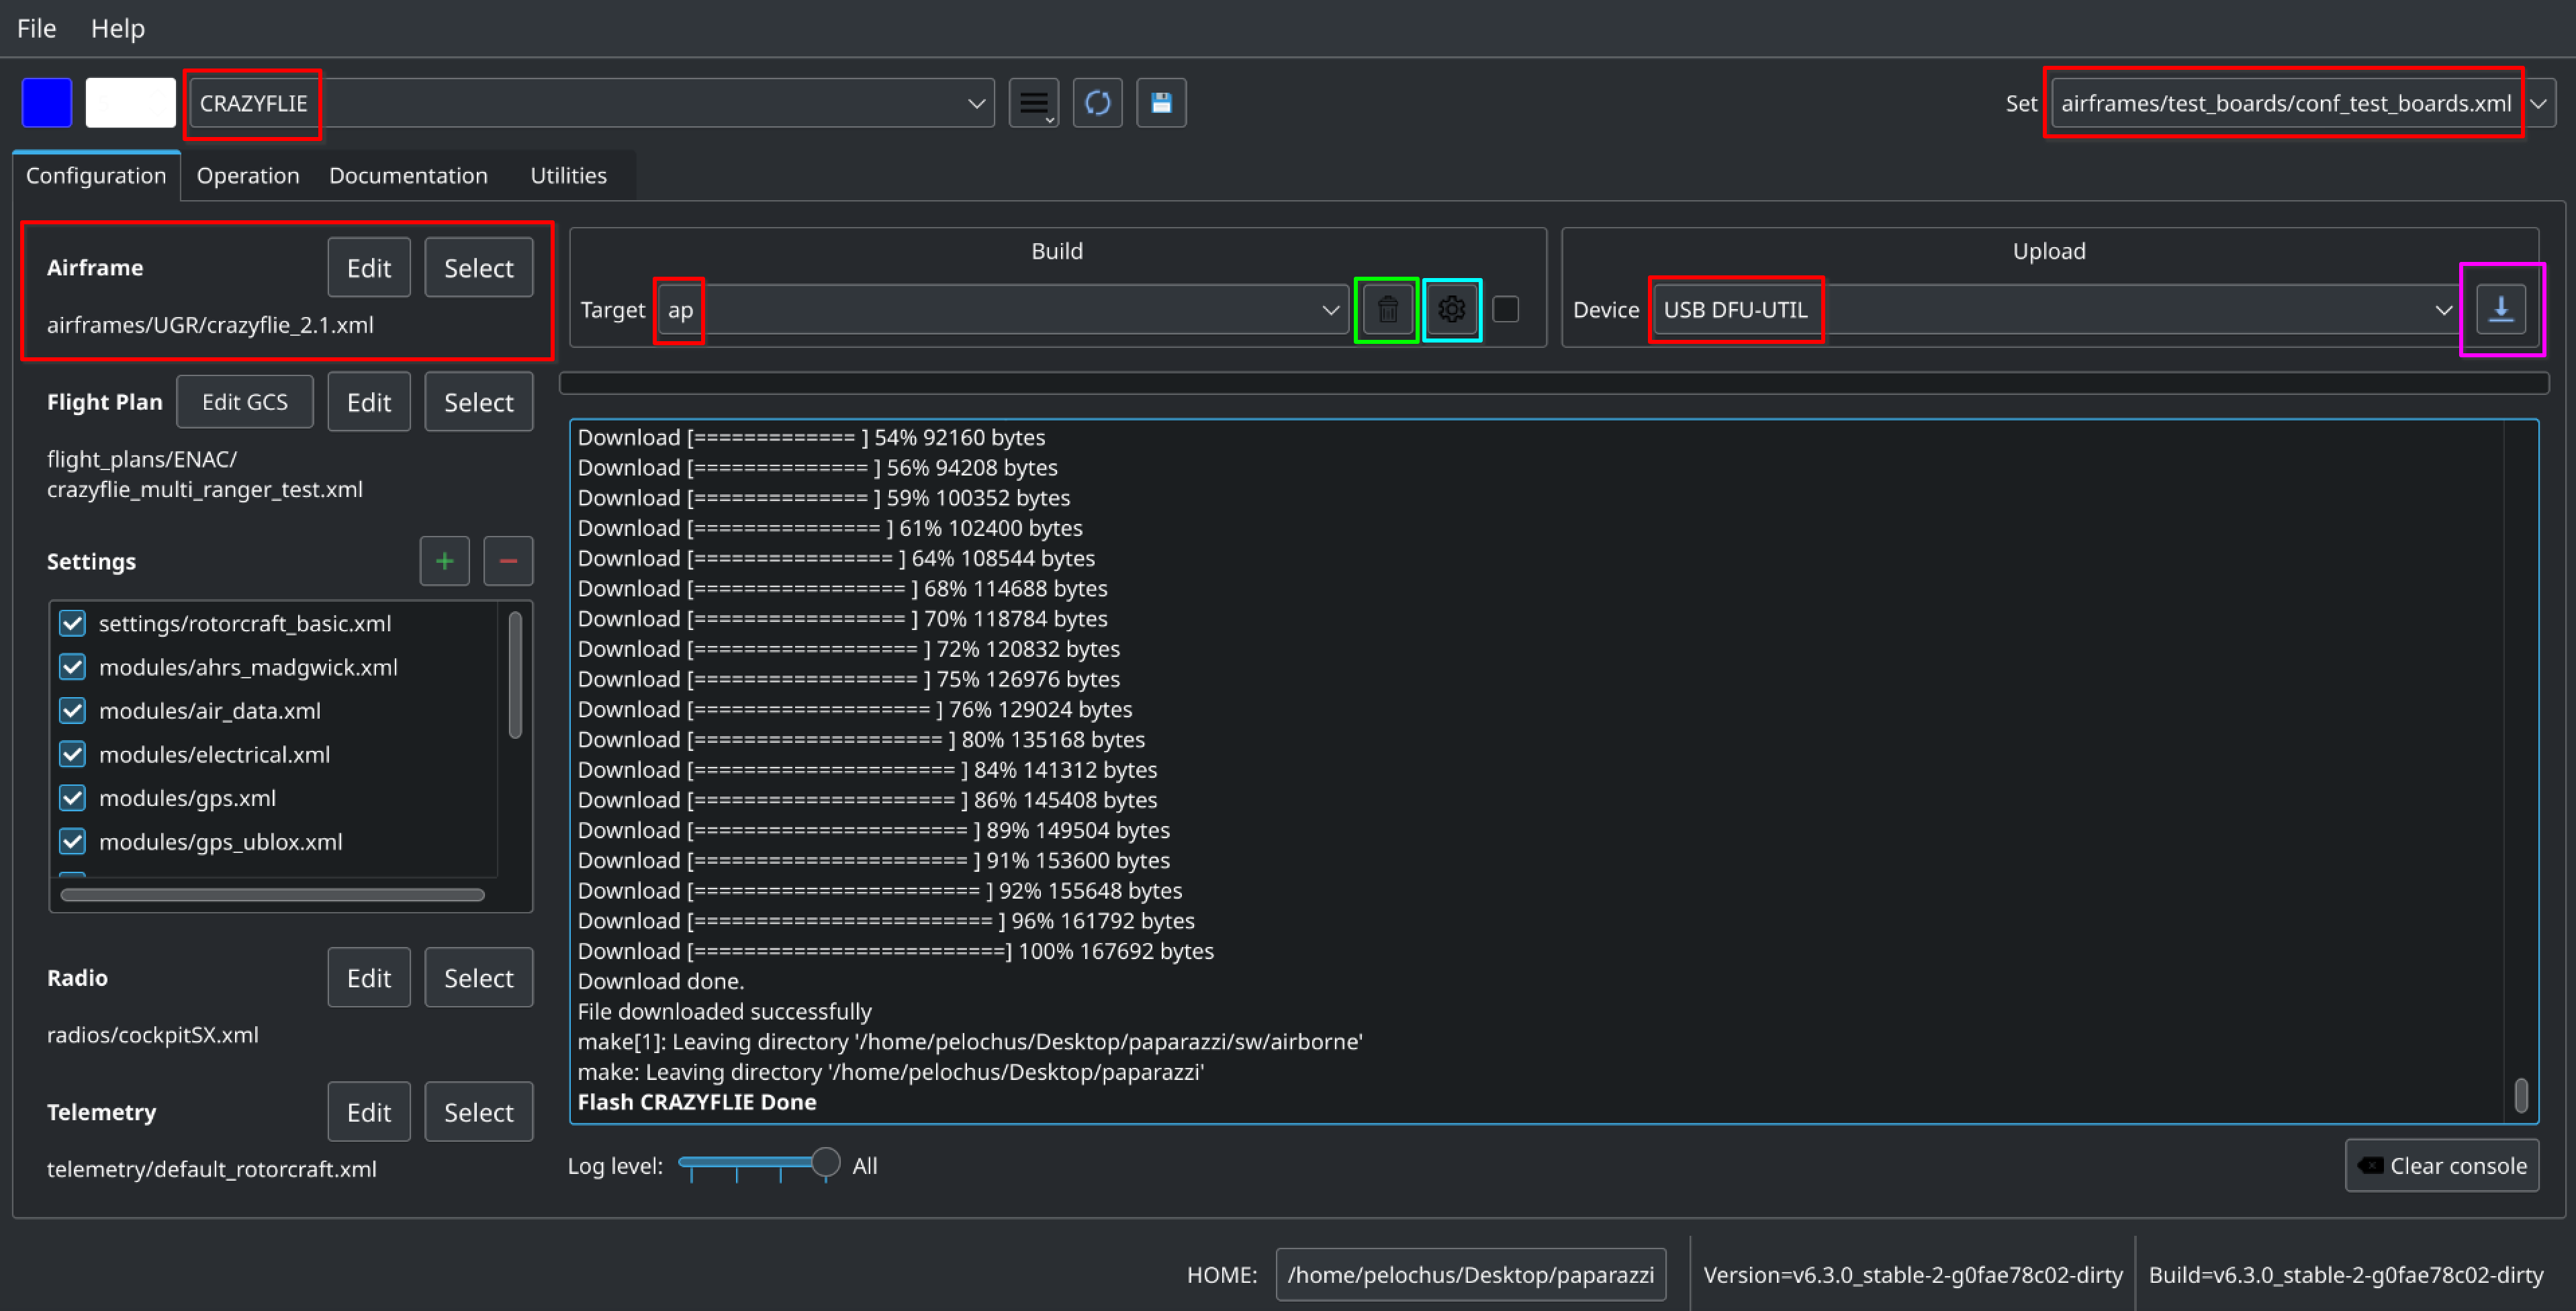
\includegraphics[width=0.99\textwidth]{img/fig/fig2.7-flash-paparazzi.png}
    \caption{Ajustes para cargar el firmware de Crazyflie en Paparazzi}
    \label{fig:upload-firmware-crazyflie}
\end{figure}

Se seguirá la guía oficial para cargar el firmware \cite{paparazzi_crazyflie}. Previamente, es necesario utilizar una versión previa del firmware oficial para conseguir compatibilidad con el firmware de Paparazzi \cite{crazyflie-firmware-fix}.
Este procedimiento consiste en los siguientes pasos:

\begin{enumerate}
    \item Se instalan las dependencias necesarias. Se encuentran el repositorio de este TFG \cite{bt-crazyflies}.
    Para un lector que no vaya a hacer pruebas, se recomienda leer el \autoref{appendix:crazyflie_dependencies}, que contiene más detalles.

    \item Se mantiene presionado el botón de encendido del Crazyflie mientras se conecta por USB.
    Esto permite entrar en el modo DFU, que permite cambiar el firmware.

    \item Desde Paparazzi se carga el firmware acorde con la \autoref{fig:upload-firmware-crazyflie}:

    \begin{enumerate}
        \item Se ajustan los parámetros que estan en \textcolor{red}{rojo} de la misma forma.
        
        \item Se pulsa el botón resaltado en \textcolor{Green3}{verde}, para limpiar archivos, análogo de Paparazzi a hacer un \textit{make clean} al compilar un ejecutable.
        
        \item Se pulsa el botón resaltado en \textcolor{cyan}{cyan}, para autocompilar el firmware. De nuevo, podemos hacer analogía con \textit{make}.

        \item Se pulsa el botón en \textcolor{violet}{morado} para cargar finalmente el firmware en el Crazyflie. Esto no debería fallar si se han seguido correctamente los pasos para instalar dependencias.
    \end{enumerate}
\end{enumerate}

Por último, se debe probar que Paparazzi funciona en el Crazyflie. 
Se probará la conexión mediante Crazyradio. Se siguen los siguientes pasos:

\begin{enumerate}
    \item Para empezar, es necesario haber instalado las dependencias.
    Se incluyen en el previamente mencionado \autoref{appendix:crazyflie_dependencies}.

    \item Siguiendo la \autoref{fig:crazyradio-paparazzi-center} 
    podemos conectar un Crazyflie a Paparazzi Center usando la Crazyradio.
    Se siguen los siguientes pasos:

    \begin{enumerate}
        \item Se añade uso del Crazyradio 2.0 mediante el menú \textit{Add Tool - Crazyradio/IvyBridge}.
        Esto añade la configuración marcada en \textcolor{red}{rojo}.
        
        \item Similarmente, desde el menú \textit{Add Tool - Messages} se añade la configuración marcada en \textcolor{Green3}{verde}. 
        Además aparece la ventana señalada en \textcolor{violet}{morado} tras seleccionar el módulo, que muestra la recepción y envío de datos.
    \end{enumerate}
\end{enumerate}

\begin{figure}[!h]
    \centering
    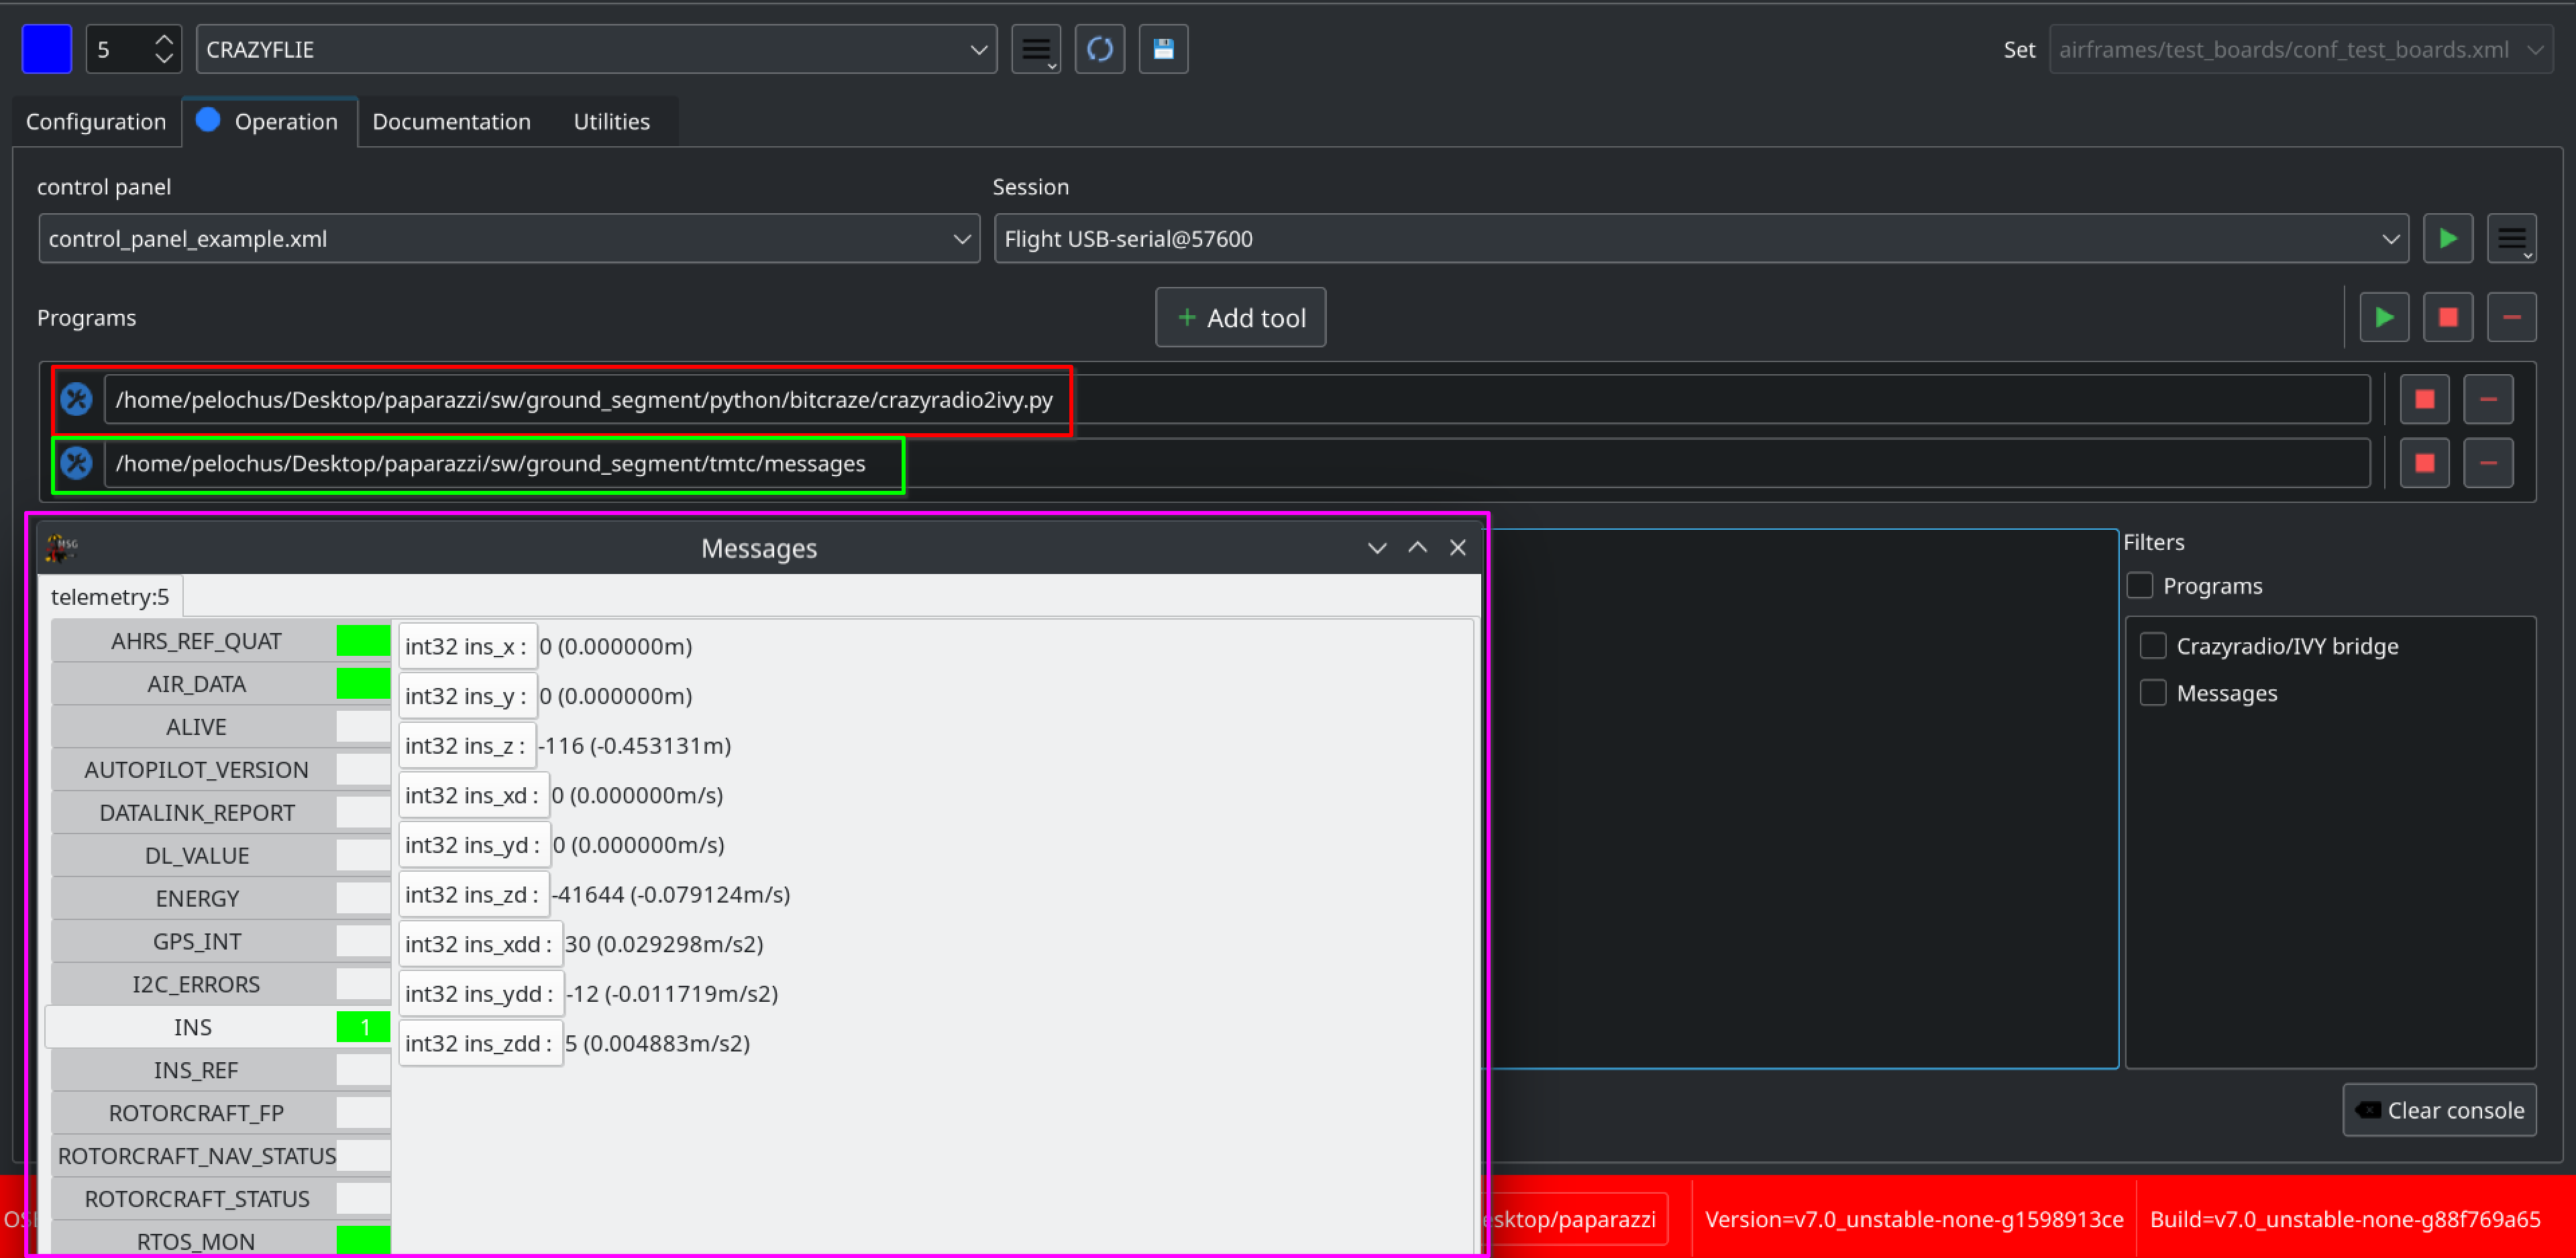
\includegraphics[width=0.85\textwidth]{img/fig/fig2.8-radio-connection.png}
    \caption{Conexión del Crazyradio al Crazyflie mediante Paparazzi}
    \label{fig:crazyradio-paparazzi-center}
\end{figure}

%%%%%%%%%%%%%%%%%%%%%%%%%%%%%%%%%%%%%%%%%%%%%%%%%%%%%%%%%%%%%%%%%%%%%%%%%%%%%%%%%%%%%%%%%%%%%%%%%%%%%%%%%%%%%%%%%
%%%%%%%%%%%%%%%%%%%%%%%%%%%%%%%%%%%%%%%%%%%%%%%%%%%%%%%%%%%%%%%%%%%%%%%%%%%%%%%%%%%%%%%%%%%%%%%%%%%%%%%%%%%%%%%%%
%%%%%%%%%%%%%%%%%%%%%%%%%%%%%%%%%%%%%%%%%%%%%%%%%%%%%%%%%%%%%%%%%%%%%%%%%%%%%%%%%%%%%%%%%%%%%%%%%%%%%%%%%%%%%%%%%

\section{Desarrollo básico en Paparazzi}

Es importante entender como se desarrolla módulos de control en Paparazzi. 
Los módulos se ocupan de controlar el UAV correspondiente de la forma más génerica posible,
permitiendo que varios UAVs distintos puedan utilizar un mismo módulo. 
Además, permiten adaptar la interfaz del GCS para, por ejemplo, colocar un deslizador que permita cambiar el control de una variable como la velocidad de un UAV.

En esta sección se desarrollará un pequeño módulo de ejemplo según la guía oficial \cite{modules-paparazzi}
de Paparazzi, así se puede entender mejor como se desarrollará este TFG.

%%%%%%%%%%%%%%%%%%%%%%%%%%%%%%%%%%%%%%%%%%%%%%%%%%%%%%%%%%%%%%%%%%%%%%%%%%%%%%%%%%%%%%%%%%%%%%%%%%%%%%%%%%%%%%%%%
%%%%%%%%%%%%%%%%%%%%%%%%%%%%%%%%%%%%%%%%%%%%%%%%%%%%%%%%%%%%%%%%%%%%%%%%%%%%%%%%%%%%%%%%%%%%%%%%%%%%%%%%%%%%%%%%%
%%%%%%%%%%%%%%%%%%%%%%%%%%%%%%%%%%%%%%%%%%%%%%%%%%%%%%%%%%%%%%%%%%%%%%%%%%%%%%%%%%%%%%%%%%%%%%%%%%%%%%%%%%%%%%%%%

\subsection{Desarrollo de módulos de control}

Paparazzi define los módulos en XML. 
Este formato permite una estructura clara y modular para implementación de módulos pero no permite el desarrollo de código. 
Para solucionar esto, el código de los módulos se implementa en el lenguaje C, 
en el cual se puede implementar algoritmos de control o manejar datos de, por ejemplo, sensores. Estos XML se encuentran en \texttt{./conf/modules/}.

La principal utilidad de los módulos aparece al compilar un firmware, donde se indica que módulos se usarán para el control del dispositivo. 
Por ejemplo, un dron con GPS y acelerómetro podrá incluir el módulo de control GPS de Paparazzi y de uso del acelerómetro. 
También existen módulos génericos, que permiten para un tipo de dispositivo, incluir los módulos básicos. 
Para un rotorcraft, será por lo general módulos de control de 4 motores, IMU 
(\textit{Inertial Measurement Unit} que incluye acelerómetro y giroscopos), control por radio etc...

Aquí vemos el módulo de demostración de Paparazzi.

\begin{lstlisting}[style=CodigoXML]
<!DOCTYPE module SYSTEM "module.dtd">

<module name="demo_module">
  <doc>
    <description>Demo module</description>
  </doc>
  <header>
    <file name="demo_module.h"/>
  </header>
  <init fun="init_demo()"/>
  <periodic fun="periodic_1Hz_demo()" freq="1." start="start_demo()" stop="stop_demo()" autorun="TRUE"/>
  <periodic fun="periodic_10Hz_demo()" period="0.1" start="start_demo()" stop="stop_demo()" autorun="FALSE"/>
  <makefile>
    <raw>
#Example of RAW makefile part
    </raw>
    <define name="DEMO_MODULE_LED" value="2"/>
    <file name="demo_module.c"/>
  </makefile>
  <makefile target="demo">
    <define name="SOME_FLAG"/>
    <configure name="SOME_DEFINE" value="bla"/>
  </makefile>
</module>
\end{lstlisting}

Por otro lado, es importante entender que la programación de los módulos esta en C. 
Estos archivos, por su parte, se encuentran en 
\texttt{./sw/airborne/modules/}
Por ejemplo, veamos el código C para el módulo de demostración:

\begin{lstlisting}[style=CodigoC]
#include "demo_module.h"
#include "led.h"

void init_demo(void)
{
  // this part is already done by led_init in fact
  LED_INIT(DEMO_MODULE_LED);
  LED_OFF(DEMO_MODULE_LED);
}

void periodic_1Hz_demo(void)
{
  LED_TOGGLE(DEMO_MODULE_LED);
}

void periodic_10Hz_demo(void)
{
  LED_TOGGLE(DEMO_MODULE_LED);
}

void start_demo(void)
{
  LED_ON(DEMO_MODULE_LED);
}

void stop_demo(void)
{
  LED_OFF(DEMO_MODULE_LED);
}
\end{lstlisting}

En conjunto, ambos archivos previos mostrados permiten generar automáticamente el encendido y apagado de un LED de forma periódica en un sistema usando el firmware de Paparazzi. 
Como bien se ha explicado antes, se puede diferenciar de forma que el archivo C permite generar la lógica mínima de control (en este caso, de los LEDs) 
y el archivo XML añade documentación, ajustes para compilación, frecuencia o periodicidad de cada función... entre otras funciones.

La razón del uso de archivos de XML, además de modularidad y claridad, es debido al uso extendido de ChibiOS en Paparazzi \cite{chibios-paparazzi}, 
un sistema operativo de tiempo real que se ocupa de ejecutar las funciones de forma periódica como bien permite definir el XML, 
utilizando, como es propio de un sistema RT, diversos hilos de ejecución. 

Existe la posibilidad de no usar ChibiOS y utilizar un programa en bucle, no obstante, no es el comportamiento más usado, ni generalmente preferible. 
La plataforma \textbf{Crazyflie 2.1 en Paparazzi utiliza ChibiOS}. 

Finalmente, hay que añadir al archivo de configuración del firmware del Crazyflie en Paparazzi este pequeño trozo de código para que, en este caso el Crazyflie, pueda ejecutar el módulo de demostración:

\begin{lstlisting}[style=CodigoXML]
<module name="demo_module"/>
\end{lstlisting}

En general, se puede resumir la estructura de los módulos y como se ubican en Paparazzi con el siguiente diagrama:

\begin{figure}[h]
    \centering
    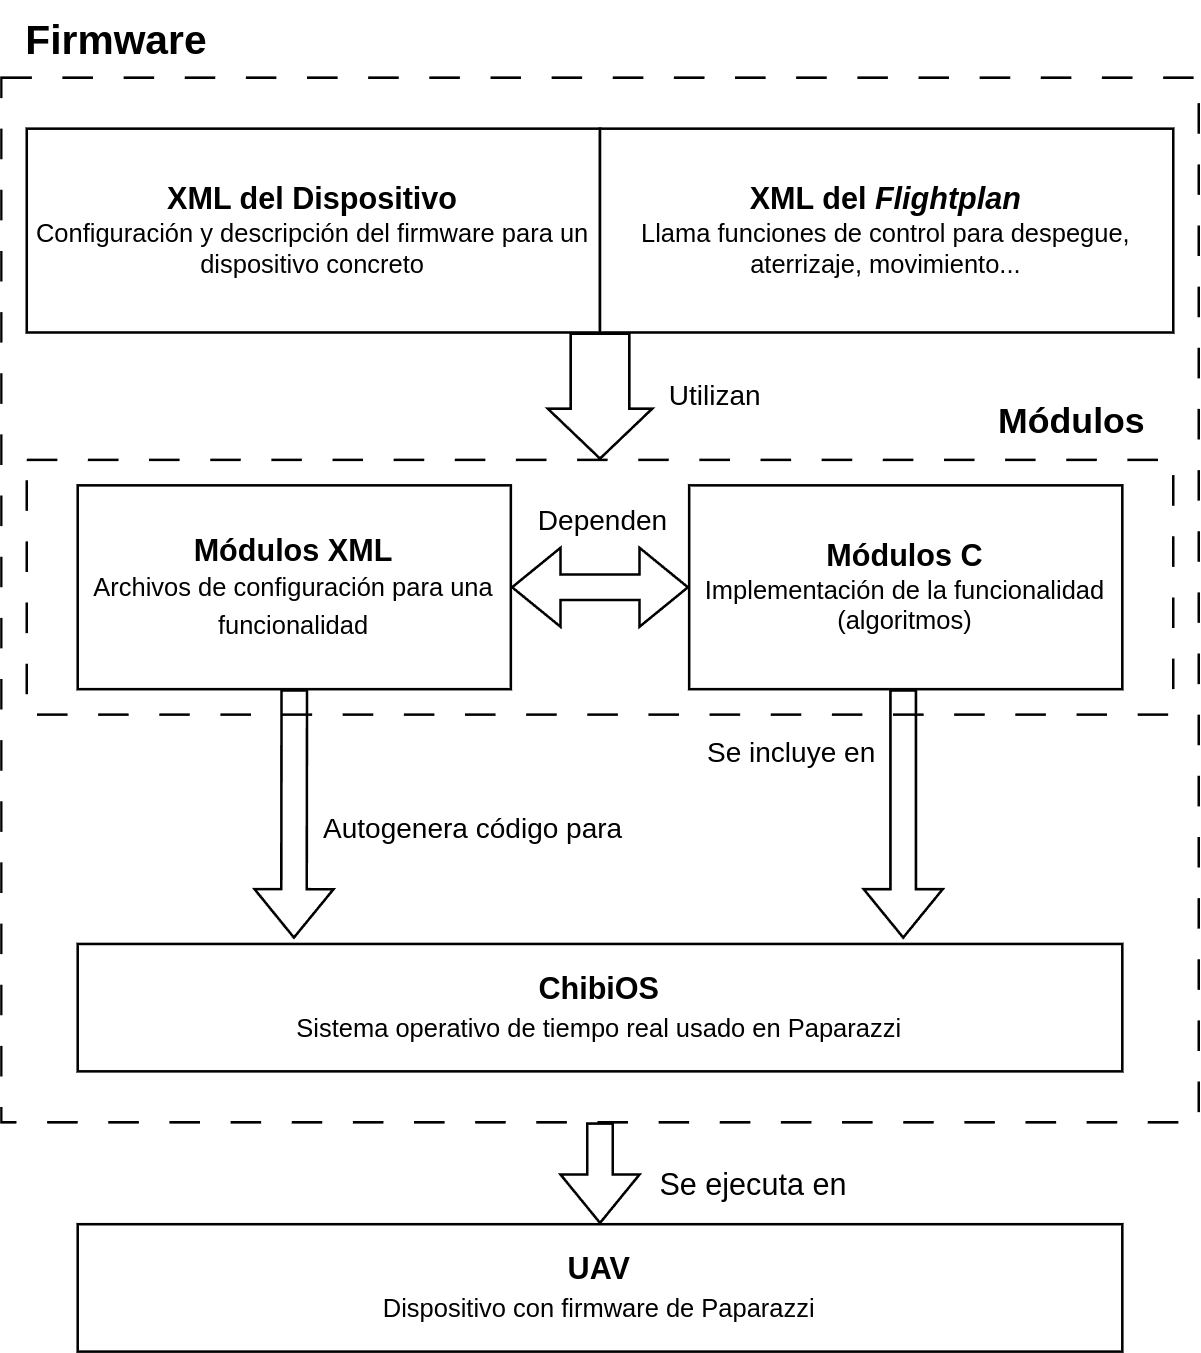
\includegraphics[width=0.72\textwidth]{img/fig/fig2.9-firmware-paparazzi.png}
    \caption{Estructura del firmware de Paparazzi}
    \label{fig:firmware-paparazzi}
\end{figure}

%%%%%%%%%%%%%%%%%%%%%%%%%%%%%%%%%%%%%%%%%%%%%%%%%%%%%%%%%%%%%%%%%%%%%%%%%%%%%%%%%%%%%%%%%%%%%%%%%%%%%%%%%%%%%%%%%
%%%%%%%%%%%%%%%%%%%%%%%%%%%%%%%%%%%%%%%%%%%%%%%%%%%%%%%%%%%%%%%%%%%%%%%%%%%%%%%%%%%%%%%%%%%%%%%%%%%%%%%%%%%%%%%%%
%%%%%%%%%%%%%%%%%%%%%%%%%%%%%%%%%%%%%%%%%%%%%%%%%%%%%%%%%%%%%%%%%%%%%%%%%%%%%%%%%%%%%%%%%%%%%%%%%%%%%%%%%%%%%%%%%

\subsection{Uso de módulos en una simulación}

En esta sección se verá en ejecución el módulo de demostración de la sección anterior. 
Los módulos permiten añadir comportamientos y funcionalidades extra a los dispositivos con Paparazzi. 
Normalmente, este comportamiento se puede observar desde Paparazzi GCS. 
En la siguiente figura podemos ver el módulo de demostración en Paparazzi GCS.

\begin{figure}[h]
    \centering
    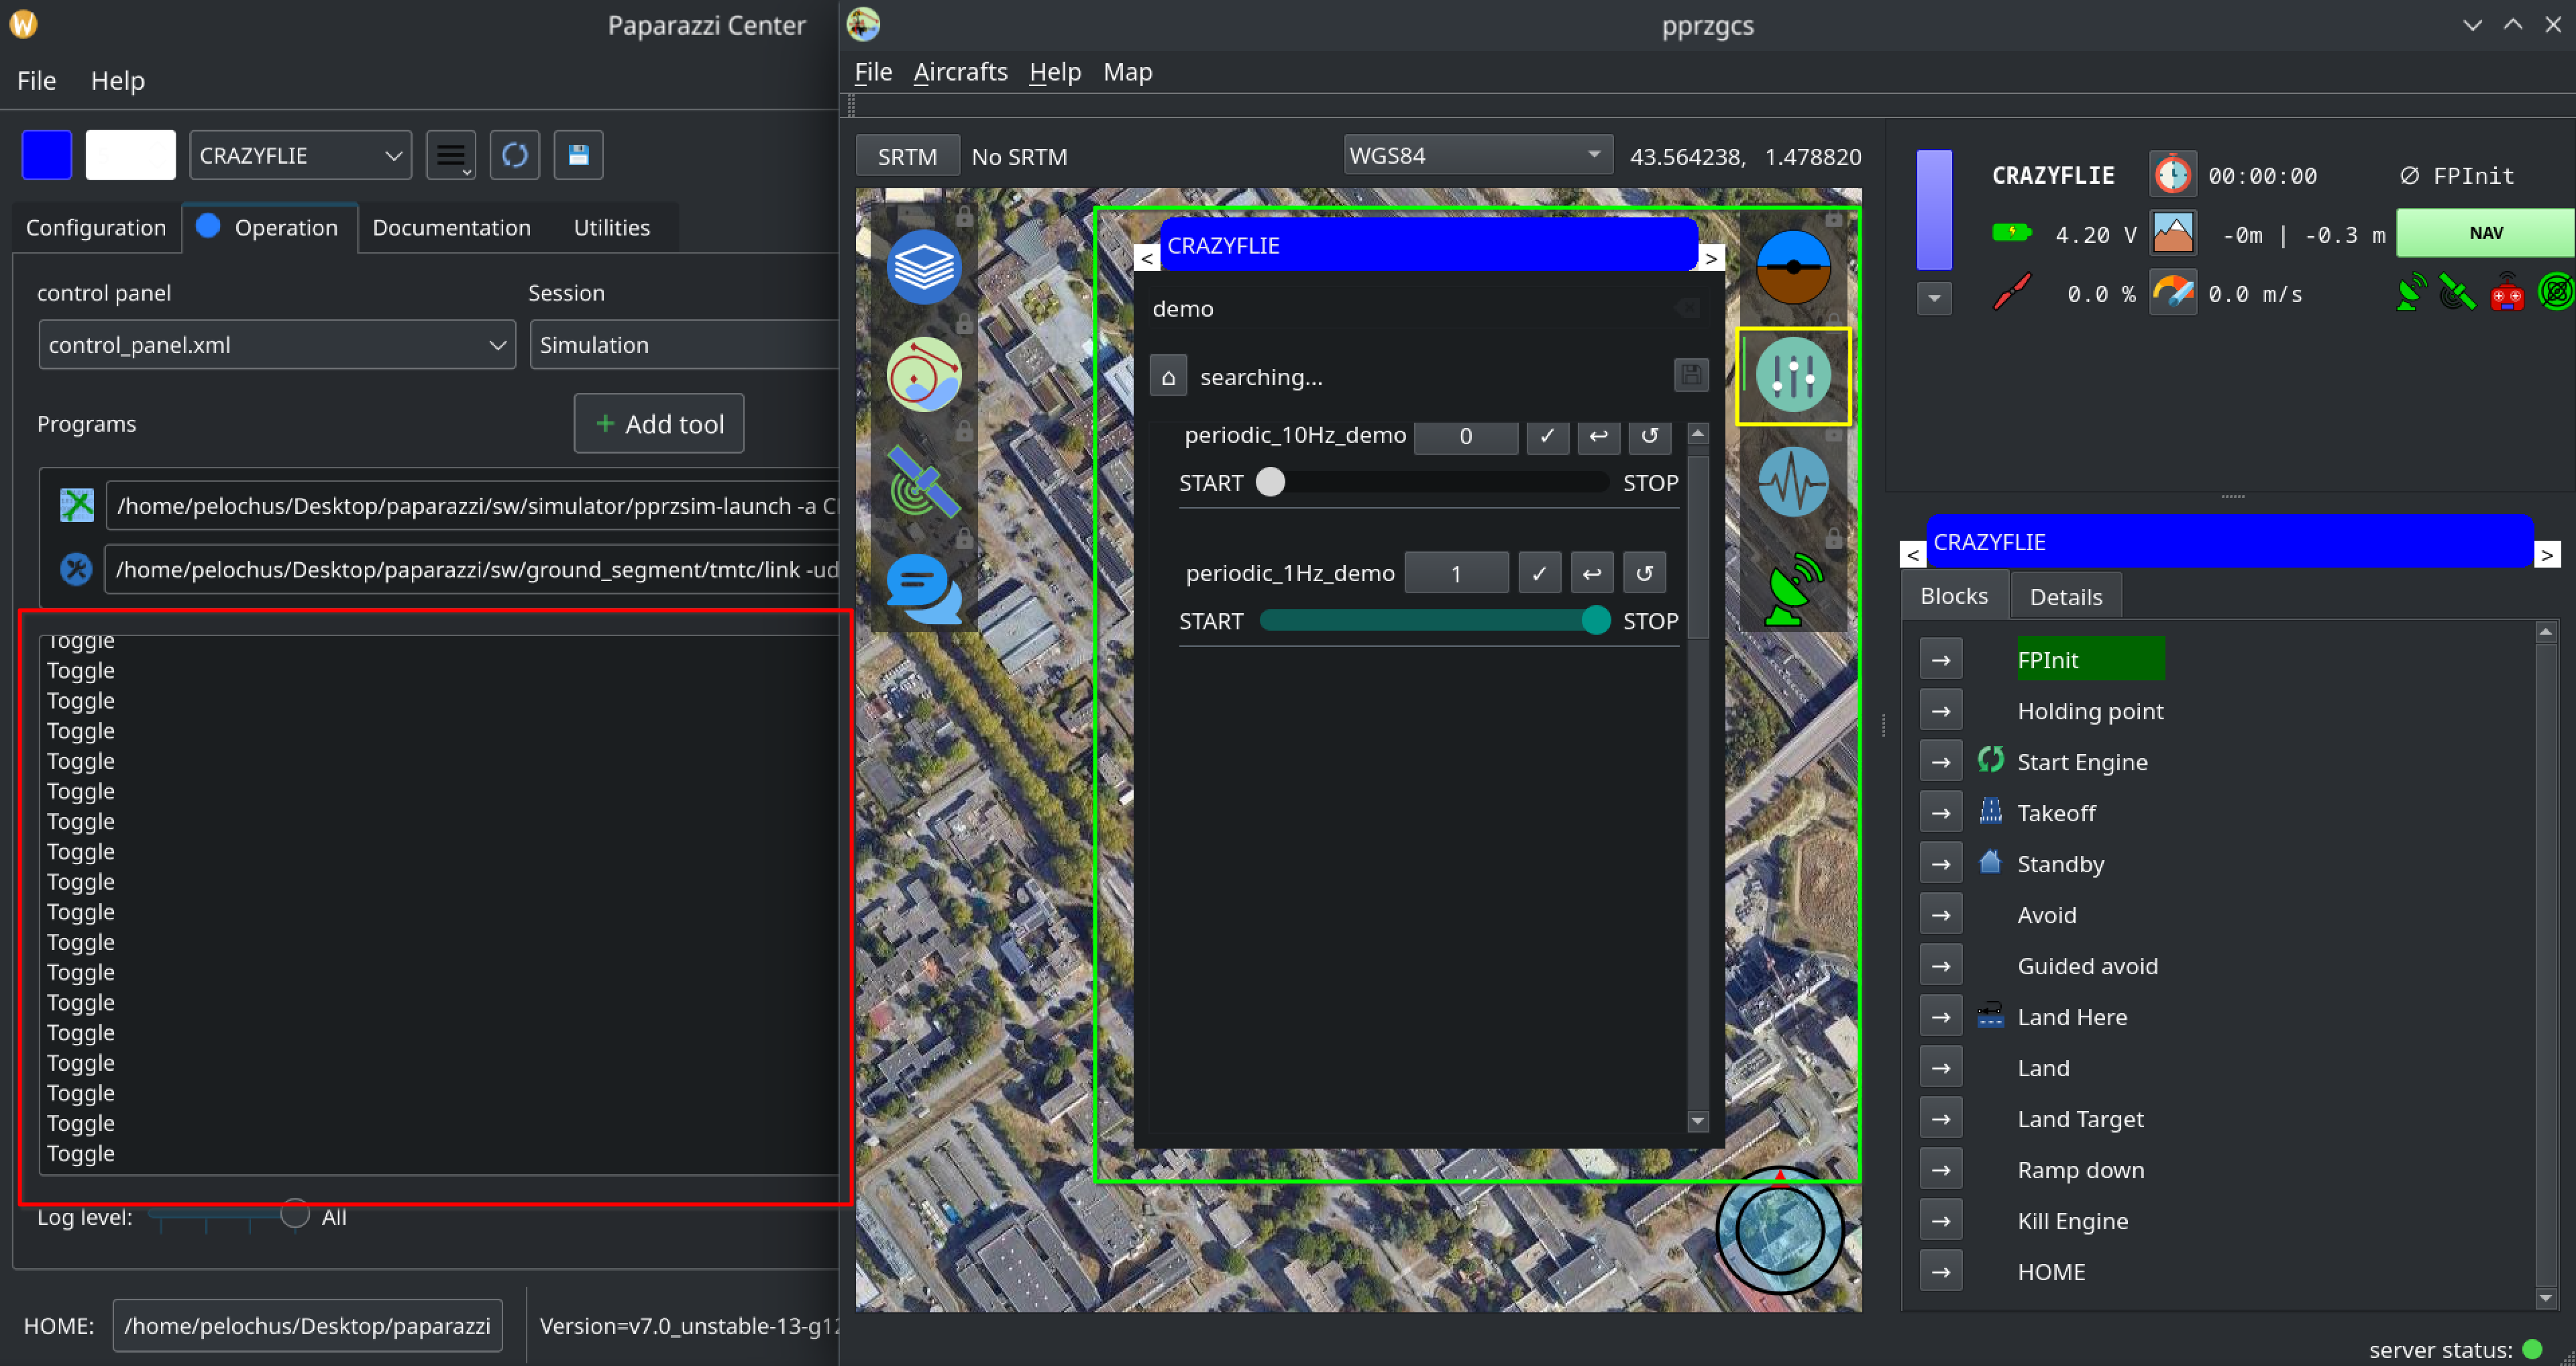
\includegraphics[width=0.99\textwidth]{img/fig/fig2.10-demo-module.png}
    \caption{Módulo de demostración en Paparazzi}
    \label{fig:demo-module-paparazzi}
\end{figure}

Si nos fijamos en la figura, podemos dividir por las siguientes partes:

\begin{enumerate}
    \item Se asume que se parte de una simulación, con Paparazzi GCS ya ejecutándose

    \item Desde el menú rodeado en color \textcolor{Green3}{verde}, podemos ajustar parámetros del módulo. 
    Para mostrar este menú se presiona el botón rodeado en \textcolor{Gold3}{amarillo}.
    
    \item Por último, podemos ver los resultados en la terminal rodeada en \textcolor{red}{rojo}.
    Al ser una simulación, simplemente se imprime por pantalla lo que se supone que se esta haciendo,
    en este caso cambiar el LED de estado cada segundo.
\end{enumerate}

Con los Crazyflies montados, funcionales con Paparazzi y entendido el funcionamiento básico de este, 
el siguiente capítulo consistirá en empezar el desarrollo para este dron en el marco de Paparazzi.
    \chapter{Control de un Crazyflie}

Dado un conocimiento básico de Paparazzi, este capítulo se centra en la 
implementación de los algoritmos de control para un sólo Crazyflie. 
Se realizarán implementaciones parcialmente agnósticas del posicionamiento entre drones,
al no ser necesaria la coordinación entre drones. 

Se entenderá el funcionamiento de un algoritmo GVF y se verá su 
implementación en Paparazzi para el Crazyflie, terminando con un buen control de este.

%%%%%%%%%%%%%%%%%%%%%%%%%%%%%%%%%%%%%%%%%%%%%%%%%%%%%%%%%%%%%%%%%%%%%%%%%%%%%%%%%%%%%%%%%%%%%%%%%%%%%%%%%%%%%%%%%
%%%%%%%%%%%%%%%%%%%%%%%%%%%%%%%%%%%%%%%%%%%%%%%%%%%%%%%%%%%%%%%%%%%%%%%%%%%%%%%%%%%%%%%%%%%%%%%%%%%%%%%%%%%%%%%%%
%%%%%%%%%%%%%%%%%%%%%%%%%%%%%%%%%%%%%%%%%%%%%%%%%%%%%%%%%%%%%%%%%%%%%%%%%%%%%%%%%%%%%%%%%%%%%%%%%%%%%%%%%%%%%%%%%

\section{Control básico}

Previo a conseguir control con algoritmos avanzados, se debe conseguir \textit{hovering}, 
es decir, que el dron flote estático a cierta altura. 
Debido a que la implementación de Paparazzi actual esta enfocada a control manual con mando, 
el PID no está debidamente ajustado. 
Conseguir hovering se reduce a un correcto ajuste del PID vertical y horizontal, 
al estar el control por PID ya implementado en el firmware del Crazyflie.

%%%%%%%%%%%%%%%%%%%%%%%%%%%%%%%%%%%%%%%%%%%%%%%%%%%%%%%%%%%%%%%%%%%%%%%%%%%%%%%%%%%%%%%%%%%%%%%%%%%%%%%%%%%%%%%%%
%%%%%%%%%%%%%%%%%%%%%%%%%%%%%%%%%%%%%%%%%%%%%%%%%%%%%%%%%%%%%%%%%%%%%%%%%%%%%%%%%%%%%%%%%%%%%%%%%%%%%%%%%%%%%%%%%
%%%%%%%%%%%%%%%%%%%%%%%%%%%%%%%%%%%%%%%%%%%%%%%%%%%%%%%%%%%%%%%%%%%%%%%%%%%%%%%%%%%%%%%%%%%%%%%%%%%%%%%%%%%%%%%%%

\subsection{PID en Paparazzi}

Paparazzi reduce el control de un rotorcraft a dos controladores PID: \textbf{uno vertical (eje Z) y otro horizontal (plano y ejes XY)}. 
El control PID en Paparazzi no difiere mucho de un control PID estándar, no obstante, cabe destacar una leve diferencia en el control PID vertical:

\begin{equation}
    m(t) = m_h + K_p e(t) + K_i \int_{0}^{t} e(t)dt + K_d \frac{de(t)}{dt}
\end{equation}

Donde:

\begin{itemize}
    \item $m(t)$ es el throttle (velocidad de los motores de 0 a 100\%) respecto al tiempo
    \item $m_h$ es el \textit{Nominal Hover Throttle}, es decir, el valor mínimo de throttle deseado. 
    Se fija a un valor muy levemente por debajo del valor mínimo para que un Crazyflie despegue. 
    Se encontró que un Crazyflie despega con un throttle de \textbf{entre 65\% y 70\%}
    \item $e(t)$ es el error respecto a la altura deseada
\end{itemize}

Nuestra principal diferencia, como se puede observar, reside en el Nominal Hover Throttle. 
Con este valor se consigue que el dron parta de un valor inicial de throttle con sentido, 
es decir, que le permita despegar del suelo. 
La siguiente figura ilustra perfectamente la idea recién explicada:

\begin{figure}[h]
    \centering
    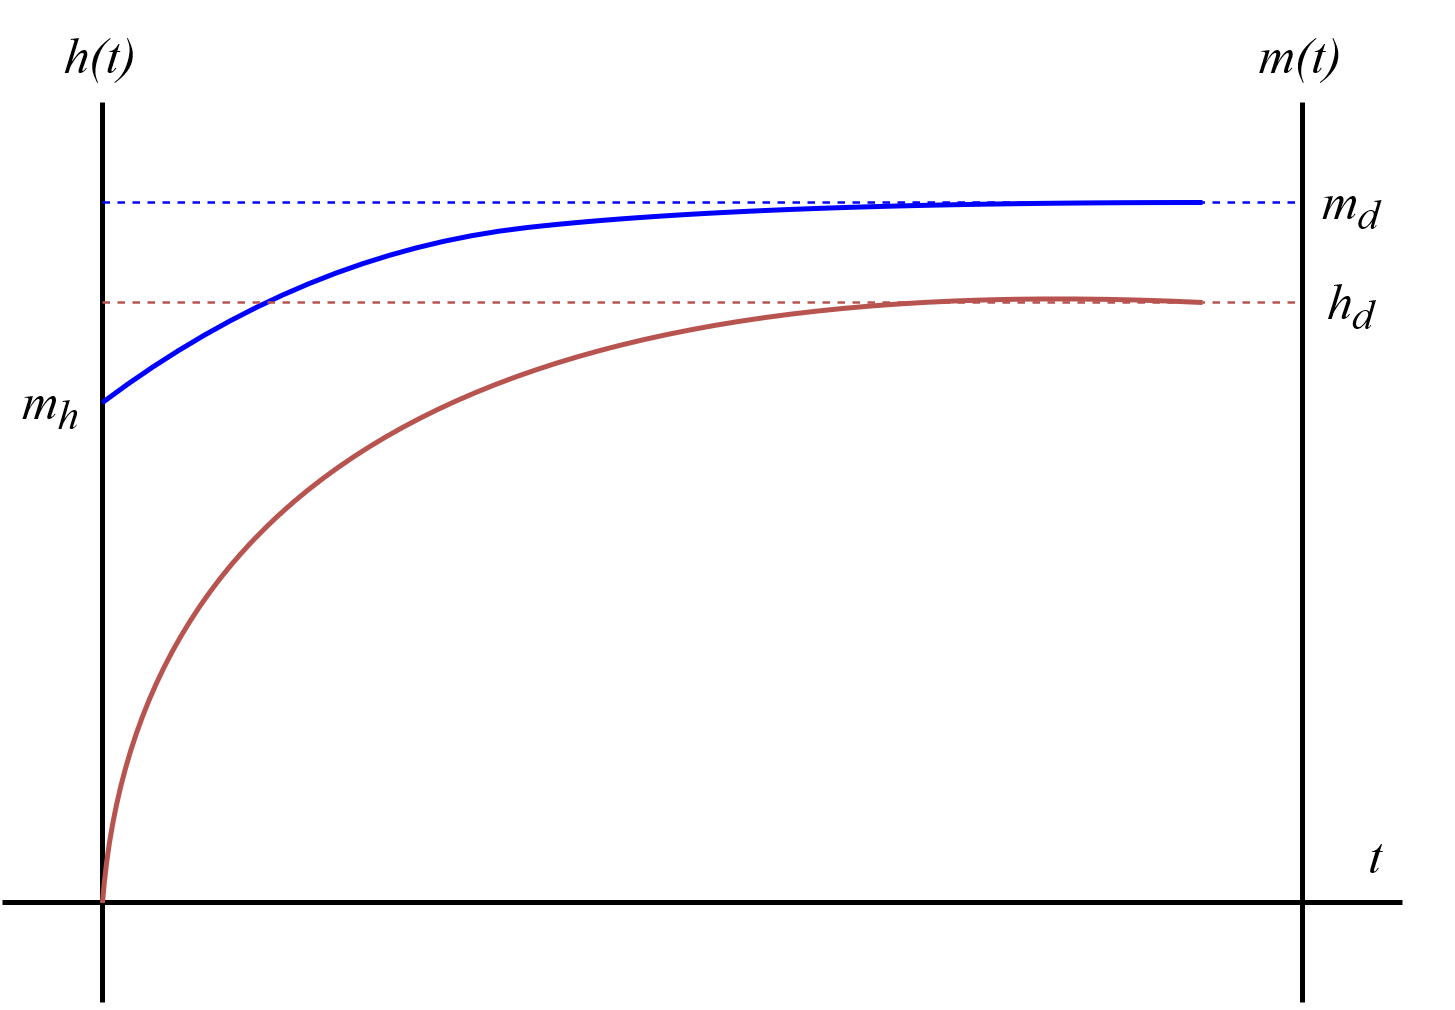
\includegraphics[width=0.95\textwidth]{img/fig/fig3.1-vertical-pid.png}
    \caption{Comparativa entre la altura conseguida por el PID y el throttle respecto al mismo tiempo. 
    En \textcolor{blue}{azul}, el throttle, en \textcolor{red}{rojo}, la altura.
    Notación: $h(t)$ altura respecto al tiempo, $h_d$ altura deseada, 
    $m_h$ es el nominal hover throttle y $m_d$ throttle para altura deseada}
    \label{fig:vertical-pid}
\end{figure}

%%%%%%%%%%%%%%%%%%%%%%%%%%%%%%%%%%%%%%%%%%%%%%%%%%%%%%%%%%%%%%%%%%%%%%%%%%%%%%%%%%%%%%%%%%%%%%%%%%%%%%%%%%%%%%%%%
%%%%%%%%%%%%%%%%%%%%%%%%%%%%%%%%%%%%%%%%%%%%%%%%%%%%%%%%%%%%%%%%%%%%%%%%%%%%%%%%%%%%%%%%%%%%%%%%%%%%%%%%%%%%%%%%%
%%%%%%%%%%%%%%%%%%%%%%%%%%%%%%%%%%%%%%%%%%%%%%%%%%%%%%%%%%%%%%%%%%%%%%%%%%%%%%%%%%%%%%%%%%%%%%%%%%%%%%%%%%%%%%%%%

\subsection{Metodología para ajuste del PID}

Idealmente, se puede automatizar el ajuste de un PID con un \textit{testbench} para drones,
que permite automáticamente ajustar los valores más precisos de manera automática. 
No obstante, las capacidades de telemetría de Paparazzi permiten diagnosticar manualmente el 
resultado de un control PID. En general, se siguió la siguiente metodología:

\begin{itemize}
    \item \textbf{Ajuste del control proporcional:} se ajusta el control proporcional hasta que se consiga que el dron despegue hasta una altura no muy lejana del objetivo, con error constante.
    \item \textbf{Ajuste del control integral:} se añade lentamente constante integral hasta que se consiga ver que esta compensa los errores del proporcional y oscila alrededor de la altura deseada.
    \item \textbf{Ajuste del control derivativo:} se ajusta la constante derivativa hasta reducir el overshoot inicial lo suficiente sin que desestabilice el control PI.
\end{itemize}

Para averiguar el nominal hover throttle se hizo a ensayo y error, debido a que es fácil averiguarlo: probar numeros de 0 a 1 (0 a 100\%) hasta que el dron de pequeños saltos.

%%%%%%%%%%%%%%%%%%%%%%%%%%%%%%%%%%%%%%%%%%%%%%%%%%%%%%%%%%%%%%%%%%%%%%%%%%%%%%%%%%%%%%%%%%%%%%%%%%%%%%%%%%%%%%%%%
%%%%%%%%%%%%%%%%%%%%%%%%%%%%%%%%%%%%%%%%%%%%%%%%%%%%%%%%%%%%%%%%%%%%%%%%%%%%%%%%%%%%%%%%%%%%%%%%%%%%%%%%%%%%%%%%%
%%%%%%%%%%%%%%%%%%%%%%%%%%%%%%%%%%%%%%%%%%%%%%%%%%%%%%%%%%%%%%%%%%%%%%%%%%%%%%%%%%%%%%%%%%%%%%%%%%%%%%%%%%%%%%%%%

\subsection{Hovering}

En la siguiente tabla tenemos los valores del PID para el controlador vertical. 
Como en cualquier control de tipo PID, tenemos las constantes proporcionales, derivativas e integrales.
Se añade en este caso el \textit{nominal hover throttle}, como bien se ha explicado previamente.

\begin{table}[h]
\centering
\begin{tabular}{l|c}
    \multicolumn{1}{c|}{\textbf{Variable}} & \textbf{Valor} \\ \hline
    $K_p$                       & 175        \\
    $K_i$                       & 30         \\
    $K_d$                       & 70         \\
    $m_h$                       & 0,625       
\end{tabular}
    \caption{Valores PID vertical}
    \label{tab:vertical_pid}
\end{table}

Paralelamente, tenemos en la siguiente tabla los valores para el PID horizontal, 
que se ocupa de evitar que el Crazyflie se mueva en los ejes X e Y.

\begin{table}[h]
\centering
\begin{tabular}{l|c}
    \multicolumn{1}{c|}{\textbf{Variable}} & \textbf{Valor} \\ \hline
    $K_p$   & 50        \\
    $K_i$   & 20        \\
    $K_d$   & 125      
\end{tabular}
    \caption{Valores PID horizontal}
    \label{tab:horizontal_pid}
\end{table}

Con ambos PID bien ajustados, se consigue que el dron se pueda mantener estático a una altura dada:

\begin{figure}[h]
    \centering
    \includegraphics[width=0.7\textwidth]{img/fig/fig3.2-hovering-crazyflie.png}
    \caption{Crazyflie haciendo hovering}
    \label{fig:hovering-crazyflie}
\end{figure}

%%%%%%%%%%%%%%%%%%%%%%%%%%%%%%%%%%%%%%%%%%%%%%%%%%%%%%%%%%%%%%%%%%%%%%%%%%%%%%%%%%%%%%%%%%%%%%%%%%%%%%%%%%%%%%%%%
%%%%%%%%%%%%%%%%%%%%%%%%%%%%%%%%%%%%%%%%%%%%%%%%%%%%%%%%%%%%%%%%%%%%%%%%%%%%%%%%%%%%%%%%%%%%%%%%%%%%%%%%%%%%%%%%%
%%%%%%%%%%%%%%%%%%%%%%%%%%%%%%%%%%%%%%%%%%%%%%%%%%%%%%%%%%%%%%%%%%%%%%%%%%%%%%%%%%%%%%%%%%%%%%%%%%%%%%%%%%%%%%%%%

\section{Algoritmos GVF}

Entre la variedad de algoritmos de control que se puede implementar, 
se ha elegido un algoritmo GVF (\textit{Guidance Vector Field}).
Este tipo de algoritmo permite recorrer trayectorias en 2D
mediante la creación de un campo vectorial que indíca velocidad y trayectoria 
del vehículo en un punto dado. 
La base matemática de este algoritmo permite bajo consumo de recursos 
(ideal en sistemas empotrados como el Crazyflie) y adaptabilidad a cualquier figura 2D representable matemáticamente.

%%%%%%%%%%%%%%%%%%%%%%%%%%%%%%%%%%%%%%%%%%%%%%%%%%%%%%%%%%%%%%%%%%%%%%%%%%%%%%%%%%%%%%%%%%%%%%%%%%%%%%%%%%%%%%%%%
%%%%%%%%%%%%%%%%%%%%%%%%%%%%%%%%%%%%%%%%%%%%%%%%%%%%%%%%%%%%%%%%%%%%%%%%%%%%%%%%%%%%%%%%%%%%%%%%%%%%%%%%%%%%%%%%%
%%%%%%%%%%%%%%%%%%%%%%%%%%%%%%%%%%%%%%%%%%%%%%%%%%%%%%%%%%%%%%%%%%%%%%%%%%%%%%%%%%%%%%%%%%%%%%%%%%%%%%%%%%%%%%%%%

\subsection{Fundamentos matemáticos}

Como bien se ha explicado previamente, un algoritmo GVF trata de recorrer 
un camino o trayectoria mediante un campo vectorial. 
Matemáticamente, podemos definir un camino $\mathcal{P} \subseteq \mathds{R}^2$
donde $\varphi(p) : \mathds{R}^2 \rightarrow \mathds{R}$
mediante la siguiente ecuación implícita:

\begin{equation}
    \mathcal{P} := \{ p : \varphi(p) = 0\}
\end{equation}

Esta representación, extraída de \cite{gvf-hector} permite ocupar todo el 
plano $\mathds{R}^2$ mediante las curvas de nivel $\{ p : \varphi(p) = c\}$, 
donde la curva que verifica $c = 0$ es la deseada. Con esta representación, a su vez, 
podemos representar el error de distancia (no tiene porque coincidir con la distancia euclídea)
del vehículo respecto a la curva deseada como:

\begin{equation}
    e(p) := \varphi(p) \in \mathds{R}
\end{equation}

Este error, nos permite variar las componentes de un vector de forma que podamos, 
en función de como de grande sea $e(p)$, incrementar o decrementar la \textit{agresividad} 
con la cual el vehículo se aproximará a la curva de nivel deseada. 
Ello, junto a una constante $k_e$ que permitirá variar la agresividad general, concluye 
en el siguiente campo vectorial de guiado propuesto por los autores de \cite{gvf-hector}:

\begin{equation} \label{eq: GVF}
    \dot{p}_d := \tau(p) - k_e e(p) n(p)
\end{equation}

Donde $\dot{p}_d$ es el vector de velocidad deseada, $\tau(p)$ es la tangente de este vector y
$n(p)$ es la componente normal del mismo vector. La siguiente figura explica gráficamente
todo lo explicado hasta ahora:

\begin{figure}[h]
    \centering
    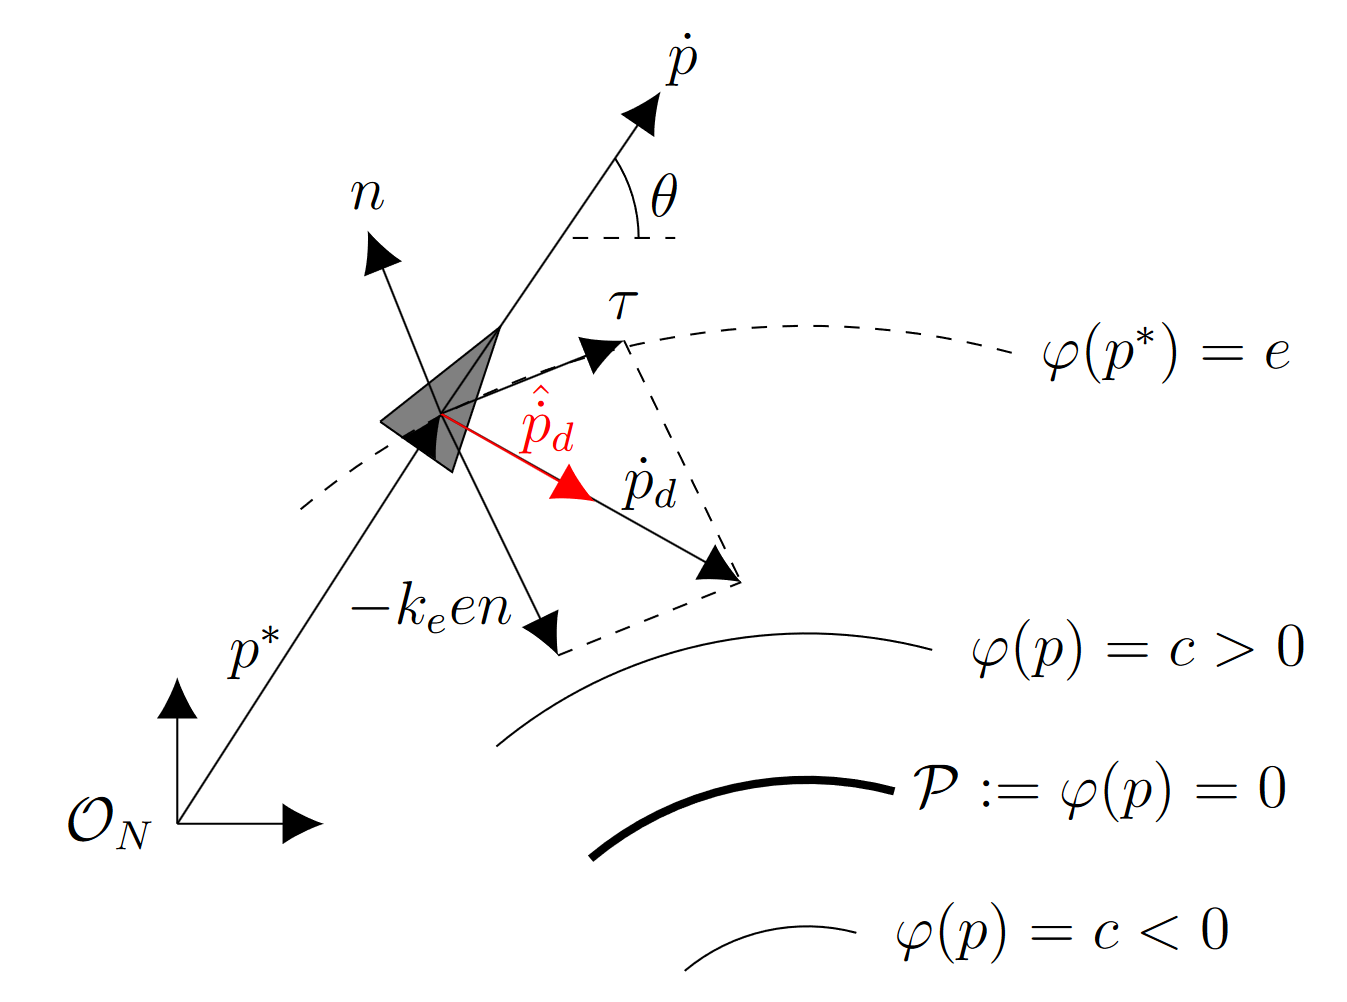
\includegraphics[width=0.7\textwidth]{img/fig/fig3.3-gvf-diagram.png}
    \caption{Representación gráfica de un vehículo bajo el efecto de un GVF. 
    Imagen extraída de \cite{tfm-jesus} y basado en \cite{gvf-hector}.}
    \label{fig:gvf-diagram}
\end{figure}

En esta figura se debe entender también lo siguiente:

\begin{itemize}
    \item $p^*$ es el punto en el plano donde se encuentra el vehículo.
    \item $\dot p$ es la velocidad actual del vehículo.
    \item $\mathcal{O}_N$ es el origen de coordenadas.
    \item $\hat{\dot{p}}_d$ es el vector con módulo normalizado a la unidad (ocasionalmente interesa solo dirección y sentido del vector) de la velocidad deseada.
    \item Tanto $n$ como $\tau$ son calculadas mediante $\nabla\varphi(p^*)$.
\end{itemize}

Como podemos observar en la figura, el resultado $\dot p_d$ tiende hacia la curva 
$\varphi(p) = 0$, es decir, el camino deseado $\mathcal{P}$. 
Es intuitivo observar que, variando la constante $k_e$ y en función de la 
curva de nivel $e$, el resultado de $\dot p_d$ será más normal (perpendicular) 
respecto al camino deseado $\mathcal{P}$, aumentando la previamente llamada agresividad.

%%%%%%%%%%%%%%%%%%%%%%%%%%%%%%%%%%%%%%%%%%%%%%%%%%%%%%%%%%%%%%%%%%%%%%%%%%%%%%%%%%%%%%%%%%%%%%%%%%%%%%%%%%%%%%%%%
%%%%%%%%%%%%%%%%%%%%%%%%%%%%%%%%%%%%%%%%%%%%%%%%%%%%%%%%%%%%%%%%%%%%%%%%%%%%%%%%%%%%%%%%%%%%%%%%%%%%%%%%%%%%%%%%%
%%%%%%%%%%%%%%%%%%%%%%%%%%%%%%%%%%%%%%%%%%%%%%%%%%%%%%%%%%%%%%%%%%%%%%%%%%%%%%%%%%%%%%%%%%%%%%%%%%%%%%%%%%%%%%%%%

\subsection{Algoritmos GVF para rotorcrafts}

Aunque GVF se puede aplicar a cualquier vehículo, los autores de \cite{gvf-hector}
continuan aportando una solución específica para un \textit{fixedwing UAV} 
el cual solo puede modificar sus ángulos de \textit{roll} y \textit{pitch} 
haciendo un movimiento usando la \textbf{velocidad angular ($\omega$)}. 

Por contraparte, un rotorcraft puede modificar su \textit{yaw} y 
puede realizar movimientos más bruscos debido a su capacidad de moverse lateralmente, 
permitiendo mucho mejor control en general. 
Se propone utilizar las \textbf{velocidades en los ejes X e Y} para control de los motores del dron,
ya que las velocidades son ya calculadas en GVF, 
se consigue una aplicación directa de una de las variables ya calculadas. 

Paparazzi incluye un algoritmo de control llamado \textbf{INDI} (\textit{Incremental Nonlinear Dynamic Inversion})
\cite{indi-paparazzi}
que se ocupa del control de forma transparente en base a una posición, velocidad o aceleración dada. 
Gracias a este algoritmo, una vez calculada la aceleración deseada en GVF 
podemos cambiar una variable en el código para que INDI se ocupe de controlar los
motores del dron para conseguir el efecto deseado. 

Debido a la flexibilidad de INDI, se podría haber usado posición o aceleración en vez de velocidad,
pero se usó la velocidad al ser lo más intuitivo y ser un prerrequisito ya calculado para GVF.

%%%%%%%%%%%%%%%%%%%%%%%%%%%%%%%%%%%%%%%%%%%%%%%%%%%%%%%%%%%%%%%%%%%%%%%%%%%%%%%%%%%%%%%%%%%%%%%%%%%%%%%%%%%%%%%%%
%%%%%%%%%%%%%%%%%%%%%%%%%%%%%%%%%%%%%%%%%%%%%%%%%%%%%%%%%%%%%%%%%%%%%%%%%%%%%%%%%%%%%%%%%%%%%%%%%%%%%%%%%%%%%%%%%
%%%%%%%%%%%%%%%%%%%%%%%%%%%%%%%%%%%%%%%%%%%%%%%%%%%%%%%%%%%%%%%%%%%%%%%%%%%%%%%%%%%%%%%%%%%%%%%%%%%%%%%%%%%%%%%%%

\subsection{Limitaciones de GVF sin posicionamiento}

Sin añadir nada a un Crazyflie, las únicas variables que este puede calcular son la aceleración en los ejes X, Y y Z, 
la presión con un barómetro (que permite hacer aproximación de la altura) y
los ángulos de roll, pitch y yaw mediante la IMU que posee \cite{imu-wikipedia}. 

Gracias a la diversas capacidades de Paparazzi, este contiene un módulo llamado \textbf{INS} (del inglés, \textit{Inertial Navigation System}), 
que permite un cálculo aproximado de la velocidad y posición integrando la aceleración.
Desafortunadamente, la naturaleza de este algoritmo y de las operaciones de punto flotante que utiliza, 
acumulan error respecto al tiempo que no se puede corregir sin otro sistema de posicionamiento como el GPS.

Como solución, se va a utilizar uno de los módulos de Bitcraze para el Crazyflie llamado \textbf{Flow Deck v2} \cite{flow-deck}.
Este módulo contiene dos sensores esenciales: 

\begin{itemize}
    \item \textbf{Altímetro:} que sustituye las medidas aproximadas del barómetro por unas de mucha mayor precisión.
    \item \textbf{Opticflow:} cámara que permite detectar velocidades en X e Y al estar mirando hacia el suelo. Necesita que el suelo tenga textura, pero es mucho mas precisa que integrar la aceleración dada por la IMU.
\end{itemize}

\begin{figure}[h]
    \centering
    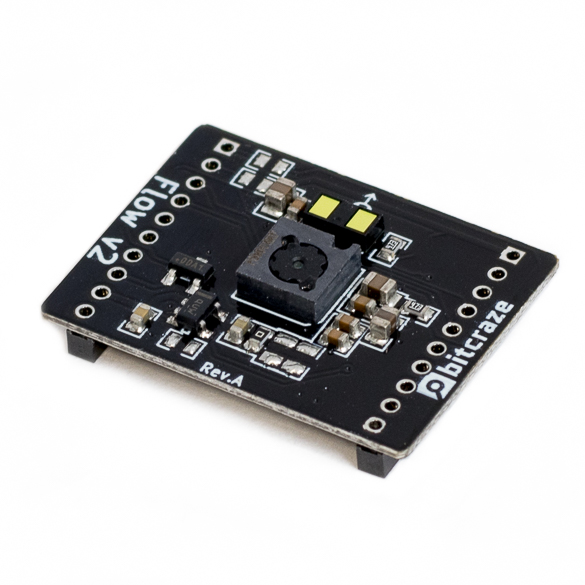
\includegraphics[width=0.4\textwidth]{img/fig/fig3.4-flow-deck.jpg}
    \caption{Flow Deck V2 de Bitcraze}
    \label{fig:flow-deck}
\end{figure}

De esta forma, aunque se sigue manteniendo el error por posición (aun se necesita integrar la velocidad, para conseguir posición),
la velocidad y la altura (imprescindibles para realizar GVF) ahora son de mayor precisión.

%%%%%%%%%%%%%%%%%%%%%%%%%%%%%%%%%%%%%%%%%%%%%%%%%%%%%%%%%%%%%%%%%%%%%%%%%%%%%%%%%%%%%%%%%%%%%%%%%%%%%%%%%%%%%%%%%
%%%%%%%%%%%%%%%%%%%%%%%%%%%%%%%%%%%%%%%%%%%%%%%%%%%%%%%%%%%%%%%%%%%%%%%%%%%%%%%%%%%%%%%%%%%%%%%%%%%%%%%%%%%%%%%%%
%%%%%%%%%%%%%%%%%%%%%%%%%%%%%%%%%%%%%%%%%%%%%%%%%%%%%%%%%%%%%%%%%%%%%%%%%%%%%%%%%%%%%%%%%%%%%%%%%%%%%%%%%%%%%%%%%

\section{Implementación del algoritmo GVF}

Paparazzi ya incluye un módulo para GVF, actualmente solo aplicado a fixedwings UAVs y rovers, los cuales son idénticos desde un punto de vista de movimiento en 2 dimensiones (utilizan ambos la velocidad angular en GVF). La estructura de los módulos de GVF en Paparazzi es la siguiente:

\vspace{8mm}

% Check this out and change it?
% https://tex.stackexchange.com/questions/5073/making-a-simple-directory-tree
\dirtree {%
.1 paparazzi.
.2 conf.
.3 modules.
.4 gvf\_module.xml \# Ajustes del módulo para GCS.
.2 $\cdots$.
.2 sw.
.3 airborne.
.4 modules.
.5 guidance.
.6 gvf.
.7 $\cdots$.
.7 gvf.c \# Código para GVF.
.7 gvf.h \# Header con definiciones para GVF.
}

%%%%%%
%%%%%%
%%%%%%
% TODO: Fix spacing from here onwards due to dirtree messing it up
%%%%%%
%%%%%%
%%%%%%

\vspace{8mm}

Además, viendo este esquema, se puede ver sobre los archivos y carpetas
lo explicado sobre la estructura de los módulos de Paparazzi en la \autoref{fig:firmware-paparazzi} de forma más visual e intuitiva.

Por ejemplo, tenemos en \texttt{conf/modules} la configuración XML del módulo de GVF
y en \texttt{sw/modules/guidance/gvf} el código (con su correspondiente algoritmia) de GVF.

En este trabajo se trabajará especialmente con los archivos \texttt{gvf.c} y \texttt{gvf.h}. 
Las siguientes subsecciones detallarán exactamente de que forma se implementa GVF para rotorcrafts en Paparazzzi.

%%%%%%%%%%%%%%%%%%%%%%%%%%%%%%%%%%%%%%%%%%%%%%%%%%%%%%%%%%%%%%%%%%%%%%%%%%%%%%%%%%%%%%%%%%%%%%%%%%%%%%%%%%%%%%%%%
%%%%%%%%%%%%%%%%%%%%%%%%%%%%%%%%%%%%%%%%%%%%%%%%%%%%%%%%%%%%%%%%%%%%%%%%%%%%%%%%%%%%%%%%%%%%%%%%%%%%%%%%%%%%%%%%%
%%%%%%%%%%%%%%%%%%%%%%%%%%%%%%%%%%%%%%%%%%%%%%%%%%%%%%%%%%%%%%%%%%%%%%%%%%%%%%%%%%%%%%%%%%%%%%%%%%%%%%%%%%%%%%%%%

\subsection{Control mínimo por GVF de un rotorcraft}

Como se mencionó previamente, el control de GVF no es agnóstico al dispositivo que lo usa y por tanto,
se ha optado por dar un control al Crazyflie comandando velocidades al controlador INDI,
que se ocupa de traducir una velocidad dada en throttle de los motores.

La implementación mínima para conseguir GVF en un rotorcraft es trivial, 
ya que GVF calcula las velocidades en los ejes X e Y y por tanto solo se debe mandar esto a INDI.
El resultado se puede ver en el siguiente trozo de código en el archivo \texttt{gvf.c}:

\begin{lstlisting}[style=CodigoC]
void gvf_control_2D(...) {
    //
    // Previous code...
    //
    
    #if defined(ROTORCRAFT_FIRMWARE)
    
      // From sw/airborne/firmware/rotorcraft/navigation.h
      nav.setpoint_mode = NAV_SETPOINT_MODE_SPEED;
      
      // md_x and md_y are normalized speeds
      nav.speed.x = gvf_control.speed * md_x;
      nav.speed.y = gvf_control.speed * md_y;
      
      // Optionally align heading with the trajectory
      if (gvf_control.align) 
          nav.heading = atan2f(md_x, md_y);
          
    #else // FIXEDWING_FIRMWARE and ROVER_FIRMWARE
    
    //
    // Following code...
    //
}
\end{lstlisting}

En este trozo de código se incluye además parte de la siguiente subsección,
pero solo \textbf{interesan las líneas 6 a 13}, que son las que se ocupan de mandar la velocidad
(calculada previamente en la misma función) 

%%%%%%%%%%%%%%%%%%%%%%%%%%%%%%%%%%%%%%%%%%%%%%%%%%%%%%%%%%%%%%%%%%%%%%%%%%%%%%%%%%%%%%%%%%%%%%%%%%%%%%%%%%%%%%%%%
%%%%%%%%%%%%%%%%%%%%%%%%%%%%%%%%%%%%%%%%%%%%%%%%%%%%%%%%%%%%%%%%%%%%%%%%%%%%%%%%%%%%%%%%%%%%%%%%%%%%%%%%%%%%%%%%%
%%%%%%%%%%%%%%%%%%%%%%%%%%%%%%%%%%%%%%%%%%%%%%%%%%%%%%%%%%%%%%%%%%%%%%%%%%%%%%%%%%%%%%%%%%%%%%%%%%%%%%%%%%%%%%%%%

\subsection{Ampliaciones al módulo de GVF en Paparazzi}

Conseguido un funcionamiento mínimo de control con un dron se añaden 
funciones nuevas para el control de este que no están integradas por defecto en Paparazzi.

\subsubsection{GVF con velocidad constante}

Utilizando GVF por defecto, la velocidad ($\dot p_d$) va en función de:

\begin{itemize}
    \item Componente tangencial de la velocidad, $\tau$

    \item Componente normal de la velocidad, $n$

    \item Constante $k_e$, que modifica la agresividad de la normal

    \item Curvas de nivel $e(p)$, que aumentan la normal en función de la curva actual
\end{itemize}

Es evidente que la velocidad no es fácilmente controlable de manera constante sin 
modificaciones al campo vectorial de guiado.
A pesar de ello, existe una solución fácil y simple para conseguir seguir un GVF con
velocidad constante sin modificar las variables previamente mencionadas.
Esta solución se reduce a comandar lo siguiente:

\begin{equation} \label{eq: Constante_GVF_Speed}
    \dot p_c := s \hat{\dot{p}}_d
\end{equation}

Donde $\dot p_c$ es la velocidad comandada al dron y $s$ es la velocidad deseada.
De esta forma, se consigue seguir el vector deseado sin modificar el campo vectorial, 
pero consiguiendo una velocidad constante.

Por otro lado, la implementación en el código es trivial. 
Se añade una función \texttt{gvf\_set\_speed(float speed)} que guarda una variable de velocidad.
Posteriormente, en la función general de GVF, 
se sustituye la velocidad deseada por el vector unitario de esta por 
la variable de velocidad previamente guardada en la función; 
en otras palabras la ecuación 3.5.

\subsubsection{Alineación con la trayectoria}

Los rotorcrafts pueden moverse libremente sobre los ejes X, Y y Z sin afectar a su yaw.
Esto permite que un Crazyflie pueda seguir trayectorias en GVF alineandose o no con ella (es decir, 
que el frontal mire hacia donde se dirige el dron o no).

\begin{figure}[h]
    \centering
    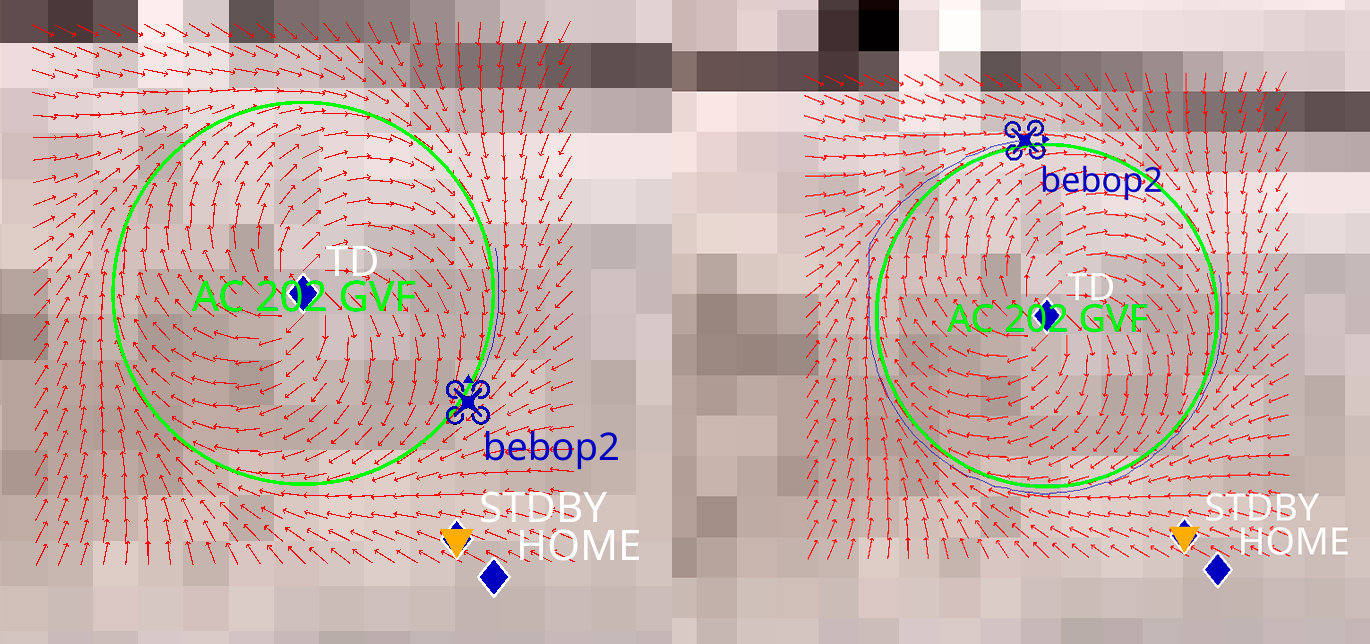
\includegraphics[width=0.7\textwidth]{img/fig/fig3.5-aligned-trajectory-gvf.png}
    \caption{Comparación de dron sin alinear (izquierda) vs alineado (derecha). Si nos fijamos en el triángulo que posee el icono del dron, en el caso de la izquierda siempre mira al norte. En el caso de la derecha, mira hacia el sentido del campo en su posición actual}
    \label{fig:align-with-trajectory}
\end{figure}

La imagen previa ilustra perfectamente en simulación las diferencias entre activar la alineación o no.
La implementación, por su parte, se realiza de manera similar al ajuste de velocidad:

\begin{itemize}
    \item Se crea la función \texttt{gvf\_set\_align(bool align)}, que guarda si se desea alinear o no

    \item Si se desea alinear, en la función principal existe el control de flujo correspondiente para cambiar el comportamiento

    \item En caso de que si se alinee, se computa el arcotangente de los vectores unitarios de velocidad en X e Y, 
    es decir, $atan2(\hat{\dot{p}}_{dx}, \hat{\dot{p}}_{dy})$. 
    Esto devuelve el ángulo deseado del yaw que será comandado al dron.
\end{itemize}
    \chapter{Coordinación con Crazyflies}

Conseguido el funcionamiento de GVF para un Crazyflie, 
se extenderá este funcionamiento de forma que dos o más Crazyflies sean coordinables,
es decir, que los recorridos que estos realicen tengan algún tipo de coordinación y dependencia mutua. Dicho de otro modo, formaciones de drones.

%%%%%%%%%%%%%%%%%%%%%%%%%%%%%%%%%%%%%%%%%%%%%%%%%%%%%%%%%%%%%%%%%%%%%%%%%%%%%%%%%%%%%%%%%%%%%%%%%%%%%%%%%%%%%%%%%
%%%%%%%%%%%%%%%%%%%%%%%%%%%%%%%%%%%%%%%%%%%%%%%%%%%%%%%%%%%%%%%%%%%%%%%%%%%%%%%%%%%%%%%%%%%%%%%%%%%%%%%%%%%%%%%%%
%%%%%%%%%%%%%%%%%%%%%%%%%%%%%%%%%%%%%%%%%%%%%%%%%%%%%%%%%%%%%%%%%%%%%%%%%%%%%%%%%%%%%%%%%%%%%%%%%%%%%%%%%%%%%%%%%

\section{Algoritmos de coordinación}

El algoritmo de coordinación elegido es una extensión de GVF para 
poder realizar formaciones circulares \cite{circular-formations}.
Además, se propone una variante de este algoritmo para poder realizar 
GVF coordinado en segmentos paralelos.

\subsection{Formación circular}

Se empezará dando un resumen de la formalización matemática dada por \cite{circular-formations}.
Para ello, se recomienda entender las nociones matemáticas de GVF previamente descritas en el capítulo 3.

Sea un conjunto de vehículos $n \in \mathbb{N}$ tal que $n \geq 2$ cuyas posiciones estan definidas por
$p_i \in \mathbb{R}^2$ para $i \in \{1 \ldots n\}$ se define el grafo no dirigido
$\mathcal{G} = \{\mathcal{V}, \mathcal{E}\}$ donde $\mathcal{V} = \{1 \ldots n \}$ es el conjunto de vértices
y $\mathcal{E} \subseteq \mathcal{V} \times \mathcal{V}$ es el conjunto de aristas.
De este grafo, nos interesa la  matriz de incidencia 
$B \in \mathbb{R}^{|\mathcal{V}| \times |\mathcal{E}|}$ que es definida de la siguiente forma:

\begin{equation}
    b_{ik} \triangleq 
    \begin{cases} 
        +1 \ para \ i = \mathcal{E}^{tail}_{k} \\
        -1 \ para \ i = \mathcal{E}^{head}_{k}  \\
        0 \ en \ otro \ caso
    \end{cases}
\end{equation}

Donde $\mathcal{E}^{tail}_{k}$ y $\mathcal{E}^{head}_{k}$ son los nodos finales e iniciales 
de una arista $\mathcal{E}_{k} = (\mathcal{E}^{tail}_{k}, \mathcal{E}^{head}_{k})$.

Con esta matriz de incidencia, podemos realizar una topología de enlaces entre vehículos de forma que
visualmente se pueda ver en la matriz que UAV toma como referencia un UAV dado.
Esto cobrará más sentido conforme se avance en esta subsección. 

Recordemos que al estar en un entorno GVF para círculos, nuestras curvas de nivel se rigen por la ecuación
$\varphi(p) = p_{x}^2 + p_{y}^2 - r^2$ donde $r \in \mathbb{R}^+$ es el radio.

Por otro lado, la coordinación se realizará en base a un ángulo, es decir, cuanto ángulo hay de desfase entre un vehículo y otro. 
Por ello, el ángulo de un vehículo $i$ en un punto $p$ respecto a $\mathcal{O}_\mathcal{N}$
del plano $\mathbb{R}^2$ viene dado por \cite{atan2}:

\begin{equation} \label{eq:theta-circular-formation}
    \theta_i(p) = atan2(p_y, p_x) \in (-\pi, \pi]
\end{equation}

Evidentemente, los ángulos que más interesan son los que hay entre un vehículo y otro, 
no el ángulo respecto a el origen de coordenadas $\mathcal{O}_\mathcal{N}$, 
solo se necesitan para calcularlos. 
Para ello, los autores de \cite{circular-formations} proponen calcular un vector de ángulos entre vehículos de la siguiente forma:

\begin{equation}
    z = B^T\theta
\end{equation}

Donde $\theta$ es el vector de ángulos calculados usando la \autoref{eq:theta-circular-formation}
y $z = \{z_1 \ldots z_k\}, \ k = |\mathcal{E}|$ es el vector de ángulos entre vehículos.
Supóngase ahora un conjunto de ángulos deseados $z^{*}_{k}$, se define $e_\theta$ como el conjunto de error
entre el ángulo actual y el deseado, regido por la ecuación:

\begin{equation}
    e_{\theta_k}(t) = z_k(t) - z_k^*
\end{equation}

Se desea que $e_\theta(t) \to 0$ para $t \to \infty$

Con toda esta base, los autores de \cite{circular-formations} terminan proponiendo la siguiente 
ecuación para control y coordinación.

\begin{equation} \label{eq:control-action-circular-formation}
    ^iu_r = k_r B_i e 
\end{equation}

Donde:

\begin{itemize}
    \item $B_i$ es la i-ésima fila de la matriz de incidencia
    \item $e$ es el vector de errores entre ángulos de vehículos
    \item $k_r \in \mathbb{R}^+$ es una ganancia de control para ajustar el resultado final  
    \item $^iu_r$ es la acción de control resultante para el radio $r$ del vehículo $i$
\end{itemize}

Finalmente, se aplica sobre el vehículo la acción de control de forma que el 
radio nuevo sea tal que permita, bajo \textbf{velocidad constante}, que los 
vehículos vayan convergiendo al ángulo deseado. 
Por tanto, aplicamos lo siguiente para cada vehículo $i$:

\begin{equation} \label{eq:applied-control-action-circular-formation}
    r_i = r_i + {^iu_r}
\end{equation}

Resumidamente, el algoritmo consiste en:

\begin{itemize}
    \item Definir un grafo $\mathcal{G}$ y usar su matriz de incidencia $B$ para definir que drones 
    se coordinarán entre sí
    \item Calcular el vector de ángulos entre vehículos $z$ en base al vector de ángulos $\theta$ respecto a 
    $\mathcal{O}_\mathcal{N}$ del plano $\mathbb{R}^2$
    \item Calcular el vector de error entre ángulos de vehículos $e$ en base a $z$ y 
    un vector de ángulos deseados $z^*$
    \item Calcular las acciones de control $u_r$ en base a $e$, $B$ y una ganancia de control $k_r$
    \item Aplicar la acción de control $u_r$ al radio actual $r$
\end{itemize}

Por simplicidad, se han obviado ciertas demostraciones, pasos y definiciones. 
Si se desea profundizar, se recomienda leer \cite{gvf-hector} y \cite{circular-formations}.

\subsection{Formación en segmentos paralelos}

La formación en segmentos paralelos consistirá en dos o más UAVs 
cada uno siguiendo su propio segmento que serán paralelos entre sí.
Es preferible usar segmentos de misma longitud.
Por simplicidad en la implementación, 
se realizará una aplicación de los segmentos de -1 a 1, 
siendo -1 un extremo y 1 el opuesto como en la figura:

\begin{figure}[!h]
    \centering
    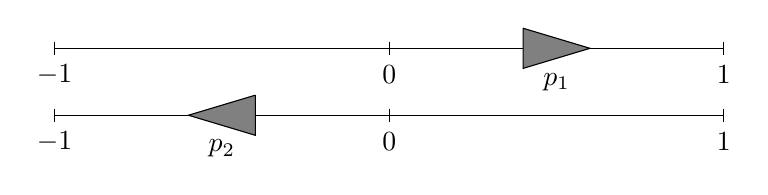
\begin{tikzpicture}[scale=0.85]
        % Dibujar el segmento de -1 a 1
        \draw[-] (-5,0) -- (5,0);
        
        % Poner las etiquetas en los extremos y en el centro
        \node at (-5, -0.4) {$-1$};
        \node at (0, -0.4) {$0$};
        \node at (5, -0.4) {$1$};
        
        % Poner las marcas en los puntos -1, 0 y 1
        \draw[-] (-5,0.1) -- (-5,-0.1);
        \draw[-] (0,0.1) -- (0,-0.1);
        \draw[-] (5,0.1) -- (5,-0.1);

        % Dron 1
        \draw[fill=gray,cm={cos(0),-sin(0),sin(0),cos(0),(0,0)}](2,0.3)--(2,-0.3)--(3,0)--(2,0.3);
        \node at (2.5, -0.5) {$p_1$};
        
        % Segundo Segmento
        % Dibujar el segmento de -1 a 1
        \draw[-] (-5,-1) -- (5,-1);
        
        % Poner las etiquetas en los extremos y en el centro
        \node at (-5, -1.4) {$-1$};
        \node at (0, -1.4) {$0$};
        \node at (5, -1.4) {$1$};
        
        % Poner las marcas en los puntos -1, 0 y 1
        \draw[-] (-5,-0.9) -- (-5,-1.1);
        \draw[-] (0,-0.9) -- (0,-1.1);
        \draw[-] (5,-0.9) -- (5,-1.1);

        % Dron 2
        \draw[fill=gray,cm={cos(0),-sin(0),sin(0),cos(0),(0,0)}](-2,-0.7)--(-2,-1.3)--(-3,-1)--(-2,-0.7);
        \node at (-2.5, -1.5) {$p_2$};
    \end{tikzpicture}
    \caption{Ejemplo de segmentos paralelos y normalizados para dos drones}
    \label{fig:parallel-segments-formation}
\end{figure}

Para realizar formación coordinada en segmentos paralelos, este trabajo
se basará en el modelo Kuramoto \cite{kuramoto-model}.
El modelo de Kuramoto se utiliza para describir la sincronización de sistemas oscilatorios 
bajo la siguiente ecuación:

\begin{equation}\label{eq:kuramoto}
    \frac{d\theta_i}{dt} = \omega_i + \frac{K}{N} \sum_{j=1}^{N} sin(\theta_j - \theta_i), 
    \ \ \ \ \ i = 1 \ldots N
\end{equation}

En base a esta ecuación y la \autoref{fig:parallel-segments-formation}, 
se propone la siguiente versión adaptada para el control en segmentos paralelos:

\begin{equation}\label{eq:segment-formation}
    v_i = v_n + K \sum_{j=1}^{N} (p_j - p_i - p^{*}_{ij}), 
    \ \ \ \ \ i = 1 \ldots N
\end{equation}

Donde:

\begin{itemize}
    \item $v_i \in \mathbb{R}$ es la velocidad resultante para el dron $i$
    \item $v_n \in \mathbb{R}$ es la velocidad nominal (o velocidad base) de los drones
    \item $K \in \mathbb{R}$ es la ganancia
    \item $N \in \mathbb{N}$ es el número total de drones
    \item $p_i$ es la posición del dron sobre el segmento normalizado, 
    por tanto $p_i \in [-1, 1], \ \forall i$
    \item $p^{*}_{ij}$ es el desajuste de la posición deseado entre el dron $i$ 
    y el dron $j$ que valdrá entre $[-2, 2]$. Por ejemplo, para 0, 
    se tiene que los drones han de estar uno al lado del otro y en paralelo.
\end{itemize}

Intuitivamente, podemos comprender el siguiente algoritmo para el caso 
$N = 2, \ K = 1, \ p^{*}_{12} = p^{*}_{21} = 0$ de la siguiente forma:

\begin{itemize}
    \item La ecuación resultante para $i = 1$ será la siguiente: $v_1 = v_n + (p_2 - p_1)$
    \item Para $i = 2$ será: $v_2 = v_n + (p_1 - p_2)$
    \item Supongamos que $v_n = 1 \ m/s$, que $p_1 = 0.5$ y que $p_2 = 0$
    \item Supongamos también que el sentido y velocidad de los drones es hacia 1 en sus segmentos, 
    es decir, actualmente están incrementando sus $p_i$
    \item Esto da como resultado $v_1 = 0.5 \ m/s$ y $v_2 = 1.5 \ m/s$, en otras palabras, la velocidad
    del dron 2 es superior y la de 1 inferior para que el dron 2 pueda alcanzar al dron 1 lo antes posible.
    Sus velocidades irán disminuyendo/aumentando en función de la cercanía entre un dron y otro en sus segmentos.
    \item Cuando $p_1 = p_2$, se tiene que $v_1 = v_2$, por tanto, ambos se mueven de forma sincronizada y paralela.
\end{itemize}

\begin{figure}[!h]
    \centering
    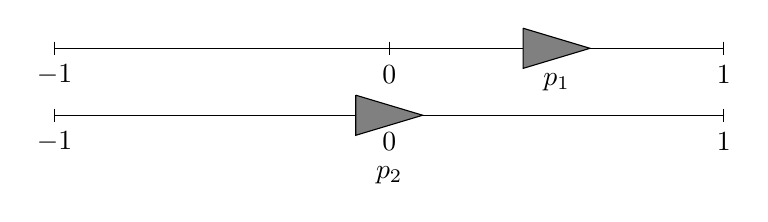
\begin{tikzpicture}[scale=0.85]
        % Dibujar el segmento de -1 a 1
        \draw[-] (-5,0) -- (5,0);
        
        % Poner las etiquetas en los extremos y en el centro
        \node at (-5, -0.4) {$-1$};
        \node at (0, -0.4) {$0$};
        \node at (5, -0.4) {$1$};
        
        % Poner las marcas en los puntos -1, 0 y 1
        \draw[-] (-5,0.1) -- (-5,-0.1);
        \draw[-] (0,0.1) -- (0,-0.1);
        \draw[-] (5,0.1) -- (5,-0.1);

        % Dron 1
        \draw[fill=gray,cm={cos(0),-sin(0),sin(0),cos(0),(0,0)}](2,0.3)--(2,-0.3)--(3,0)--(2,0.3);
        \node at (2.5, -0.5) {$p_1$};
        
        % Segundo Segmento
        % Dibujar el segmento de -1 a 1
        \draw[-] (-5,-1) -- (5,-1);
        
        % Poner las etiquetas en los extremos y en el centro
        \node at (-5, -1.4) {$-1$};
        \node at (0, -1.4) {$0$};
        \node at (5, -1.4) {$1$};
        
        % Poner las marcas en los puntos -1, 0 y 1
        \draw[-] (-5,-0.9) -- (-5,-1.1);
        \draw[-] (0,-0.9) -- (0,-1.1);
        \draw[-] (5,-0.9) -- (5,-1.1);

        % Dron 2
        \draw[fill=gray,cm={cos(0),-sin(0),sin(0),cos(0),(0,0)}](-0.5,-0.7)--(-0.5,-1.3)--(0.5,-1)--(-0.5,-0.7);
        \node at (0, -1.9) {$p_2$};
    \end{tikzpicture}
    \caption{Situación inicial para el ejemplo descrito de formación en segmentos}
    \label{fig:parallel-segments-formation-example}
\end{figure}

\subsubsection{Ajuste de la ganancia}

Al ser este algoritmo diseñado por el autor para este TFG, se propone la siguiente
forma de ajustar la ganancia:

\begin{itemize}
    \item Se supone $N = 2$ y $p^{*}_{ij} = 0$
    \item Se recomienda que la velocidad \textbf{mínima} de un dron sea 0 ($v_i = 0$). 
    En base a esto, el resultado de $K(p_j - p_i)$ deberá ser, 
    \textbf{como máximo} igual a $-v_n$
    \item Se sabe que, como máximo, $p_j - p_i = \pm 2$
\end{itemize}

En base a todo esto, podemos decir $0 = v_n - 2K$ que da 
como resultado $K = \frac{v_n}{2}$, por tanto, 
se recomienda usar una $K$ que sea la mitad de la velocidad nominal deseada.
La velocidad máxima será $v_i = v_n + Kmax(p_j - p_i) = v_n + 2 \frac{v_n}{2} = 2v_n$

Evidentemente, este método es un ejemplo para ajustar la ganancia. 
En función de los resultados deseados se preferirá un método u otro para ajustarla,
pero no se recomienda reducirla ni aumentarla mucho más, al poder haber problemas. 

%%%%%%%%%%%%%%%%%%%%%%%%%%%%%%%%%%%%%%%%%%%%%%%%%%%%%%%%%%%%%%%%%%%%%%%%%%%%%%%%%%%%%%%%%%%%%%%%%%%%%%%%%%%%%%%%%
%%%%%%%%%%%%%%%%%%%%%%%%%%%%%%%%%%%%%%%%%%%%%%%%%%%%%%%%%%%%%%%%%%%%%%%%%%%%%%%%%%%%%%%%%%%%%%%%%%%%%%%%%%%%%%%%%
%%%%%%%%%%%%%%%%%%%%%%%%%%%%%%%%%%%%%%%%%%%%%%%%%%%%%%%%%%%%%%%%%%%%%%%%%%%%%%%%%%%%%%%%%%%%%%%%%%%%%%%%%%%%%%%%%

\subsection{Comparativa entre formaciones}

Aprovechando que ya se han explicado y entendido ambos algoritmos, es interesante
comparar ambos algoritmos para ver sus similitudes. Recordemos ambas ecuaciones:

\begin{align*}
    r_i &= r_i + k_r B_i e \\
    v_i &= v_n + K \sum_{j=1}^{N} (p_j - p_i - p^{*}_{ij})
\end{align*}

Nótese que se ha expandido la \autoref{eq:applied-control-action-circular-formation} usando
la \autoref{eq:control-action-circular-formation}.

Es evidente, que hay grandes similitudes. A grandes rasgos, pueden compararse de la siguiente forma:

\begin{itemize}
    \item $r_i$ equivale a $v_i$
    \item $k_r$ equivale a $K$. 
    La principal diferencia es que en segmentos solo hay una constante para todos,
    pero se podría intercambiar por una matriz de ganancias $k_{ij}$
    \item $e$ es equivalente a $p_j - p_i - p^{*}_{ij}$. De hecho, si expandimos,
    $e = z_k - z_k^*$
    \item $B_i$ equivale indirectamente a los distintas expresiones resultantes del sumatorio 
    para todos $p^{*}_{ij}$ (esto último se puede expresar como la matriz de deajustes deseados $p^*$)
\end{itemize}
%%%%%%%%%%%%%%%%%%%%%%%%%%%%%%%%%%%%%%%%%%%%%%%%%%%%%%%%%%%%%%%%%%%%%%%%%%%%%%%%%%%%%%%%%%%%%%%%%%%%%%%%%%%%%%%%%
%%%%%%%%%%%%%%%%%%%%%%%%%%%%%%%%%%%%%%%%%%%%%%%%%%%%%%%%%%%%%%%%%%%%%%%%%%%%%%%%%%%%%%%%%%%%%%%%%%%%%%%%%%%%%%%%%
%%%%%%%%%%%%%%%%%%%%%%%%%%%%%%%%%%%%%%%%%%%%%%%%%%%%%%%%%%%%%%%%%%%%%%%%%%%%%%%%%%%%%%%%%%%%%%%%%%%%%%%%%%%%%%%%%

\section{Implementación de los algoritmos de coordinación}

Similarmente a GVF, Paparazzi ya incluye formación circular, 
pero no esta adaptada a rotorcrafts \cite{paparazzi-circular-formation}.
Adaptar esto implica diversos cambios referidos al ámbito de los rotorcrafts 
que se verán en la siguiente subsección.

%%%%%%%%%%%%%%%%%%%%%%%%%%%%%%%%%%%%%%%%%%%%%%%%%%%%%%%%%%%%%%%%%%%%%%%%%%%%%%%%%%%%%%%%%%%%%%%%%%%%%%%%%%%%%%%%%
%%%%%%%%%%%%%%%%%%%%%%%%%%%%%%%%%%%%%%%%%%%%%%%%%%%%%%%%%%%%%%%%%%%%%%%%%%%%%%%%%%%%%%%%%%%%%%%%%%%%%%%%%%%%%%%%%
%%%%%%%%%%%%%%%%%%%%%%%%%%%%%%%%%%%%%%%%%%%%%%%%%%%%%%%%%%%%%%%%%%%%%%%%%%%%%%%%%%%%%%%%%%%%%%%%%%%%%%%%%%%%%%%%%

\subsection{Adaptación de formaciones circulares}

Paparazzi ya incluye formaciones circulares utilizando un script de Python ubicado en
\texttt{sw/ground\_segment/python/gvf} llamado \texttt{circularFormation.py}.
Este script, similarmente a GVF, no tiene adaptación para rotorcrafts. 
En resumen, el script consiste en:

\begin{itemize}
    \item Ejecución del script con un párametro obligatorio que sera un archivo JSON con parámetros deseados
    \item Lectura del archivo JSON para recabar ajustes cómo los IDs internos de los vehículos en Paparazzi
    \item Sincronización del script con la instancia actual de Paparazzi. Hasta que no se encuentre todos los IDs de los UAVs funcionando bajo GVF tipo círculo el script no se comenzará a ejecutar
    \item Lectura de la telemetría recibida por los UAVs, para conseguir información como la posición actual
    \item Cálculo del algoritmo, es decir, cálculo de los ángulos entre vehículos, errores... para poder calcular el radio deseado para cada dron
    \item Se devuelve la telemetría a través de la libreria de Paparazzi para Python que permite comunicarse con los UAVs
\end{itemize}

La estructura de un archivo JSON suele ser como la siguiente:

% En realidad es JSON, pero no voy a hacer un perfil, con C vale
\begin{lstlisting}[style=CodigoC]
{
  "ids": [1,2],
  "topology": [
    [ 1],
    [-1]
  ],
  "desired_intervehicle_angles_degrees": [0],
  "gain": 10,
  "desired_stationary_radius_meters": 80
}
\end{lstlisting}

Donde podemos ver los IDs de los vehículos, la topología deseada (matriz $B$), 
ángulo deseado entre vehículos ($z^*$), ganancia ($k_r$) y el radio base deseado ($r_i$).

Para conseguir que esto también funcione para rotorcrafts y por tanto los Crazyflie, 
se han hecho los siguientes cambios:

\begin{itemize}
    \item Se añade un nuevo parámetro obligatorio al ejecutar el script.
    Este parámetro será el tipo de vehículo utilizado, en este caso, hay dos opciones:
    \begin{itemize}
        \item \textbf{Fixedwing:} la ya implementada para aviones de ala fija
        \item \textbf{Rotorcraft:} la nueva implementación para drones como el Crazyflie
    \end{itemize}
    \item Internamente en el script, se añade una condición que hará que se suscriba a los mensajes
    de \texttt{NAVIGATION} o \texttt{ROTORCRAFT\_FP} en función de el tipo de UAV deseado.
    Estos mensajes de telemetría son los encargados de mandar las posiciones relativas 
    (respecto al punto de inicio) de los fixedwing y rotorcraft, respectivamente. 
\end{itemize}

El resto del algoritmo no depende de ningún parámetro extra que pueda ser exclusivo a un tipo de UAV u otro.
Consecuentemente, no se necesitan más adaptaciones para las formaciones circulares en rotorcrafts.

%%%%%%%%%%%%%%%%%%%%%%%%%%%%%%%%%%%%%%%%%%%%%%%%%%%%%%%%%%%%%%%%%%%%%%%%%%%%%%%%%%%%%%%%%%%%%%%%%%%%%%%%%%%%%%%%%
%%%%%%%%%%%%%%%%%%%%%%%%%%%%%%%%%%%%%%%%%%%%%%%%%%%%%%%%%%%%%%%%%%%%%%%%%%%%%%%%%%%%%%%%%%%%%%%%%%%%%%%%%%%%%%%%%
%%%%%%%%%%%%%%%%%%%%%%%%%%%%%%%%%%%%%%%%%%%%%%%%%%%%%%%%%%%%%%%%%%%%%%%%%%%%%%%%%%%%%%%%%%%%%%%%%%%%%%%%%%%%%%%%%

\subsection{Implementación de formaciones en segmentos}

En base a la ya implementada formación en circulos, se ha hecho un nuevo
programa en Python que implementa la formacion en segmentos, ya que Paparazzi no incluye este programa. 
Los cambios son:

\begin{itemize}
    \item Ajustes generales al script del estilo nombres de variables, parámetros de entrada, comentarios...
    \item Cambio del algoritmo y de las clases para adaptarse a segmentos
    \item Cambios en la telemetría para sacar otros datos necesarios
    \item Solo funciona para rotorcrafts, al seguir estos un segmento de mejor forma que un fixedwing
\end{itemize}

Además, se ha cambiado la estructura del archivo JSON levemente para adaptarse al script. Por ejemplo:

\begin{lstlisting}[style=CodigoC]
{
  "ids": [8,9],
  "desired_normalized_offset": [0],
  "nominal_speed": 0.25,
  "gain": 0.15
}
\end{lstlisting}

Por último, al no ser explicado en la teoría de este algoritmo, 
se muestra aquí el trozo de código que hace la normalización del segmento:

\begin{lstlisting}[style=CodigoPython]
# Segment normalization
i = 0
for ac in self.aircraft:
    # Calculate x and y distances, from segment and current pos
    max_dist_x = ac.WP2[0] - ac.WP1[0]
    max_dist_y = ac.WP2[1] - ac.WP1[1]
    dist_x = ac.XY[0] - ac.WP1[0]
    dist_y = ac.XY[1] - ac.WP1[1]

    # Vector modulus (Pythagoras)
    max_dist = math.sqrt(max_dist_x**2 + max_dist_y**2)
    dist = math.sqrt(dist_x**2 + dist_y**2)

    # Having this, we can normalize the distance from 0 to 1
    norm_dist = dist / max_dist

    # Map segment values from range(0, 1) to range(-1, 1)
    def map_range(d, in_min, in_max, out_min, out_max):
        if (in_max == in_min):
            return 0
        else:
            return (d - in_min) * (out_max - out_min) / (in_max - in_min) + out_min
    
    self.mapped_pos[i] = map_range(norm_dist, 0, 1, -1, 1)
    i += 1
\end{lstlisting}

En resumen:

\begin{itemize}
    \item Se calculan las distancias en X y en Y
    \item Se calcula el módulo del vector de las distancias
    \item Se normaliza a 1
    \item Por último, se realiza un \textit{mapping} del vector normalizado (0 a 1) a la normalización propia (-1 a 1)
\end{itemize}

Evidentemente, existen más metodos para conseguir esta normalización (u otros tipos de normalización), 
pero se ha optado por este al ser simple de realizar, bajo coste computacional y fácil de entender. 
Funciona además, para un segmento en cualquier ángulo y dirección.

%%%%%%%%%%%%%%%%%%%%%%%%%%%%%%%%%%%%%%%%%%%%%%%%%%%%%%%%%%%%%%%%%%%%%%%%%%%%%%%%%%%%%%%%%%%%%%%%%%%%%%%%%%%%%%%%%
%%%%%%%%%%%%%%%%%%%%%%%%%%%%%%%%%%%%%%%%%%%%%%%%%%%%%%%%%%%%%%%%%%%%%%%%%%%%%%%%%%%%%%%%%%%%%%%%%%%%%%%%%%%%%%%%%
%%%%%%%%%%%%%%%%%%%%%%%%%%%%%%%%%%%%%%%%%%%%%%%%%%%%%%%%%%%%%%%%%%%%%%%%%%%%%%%%%%%%%%%%%%%%%%%%%%%%%%%%%%%%%%%%%

\section{Simulación de las formaciones}

Para acabar este capítulo, veremos los resultados en simulación de los algoritmos implementados.
Se verá tanto formaciones circulares como en segmentos. 
En el caso de las circulares, se obviará los casos reales ya que Paparazzi 
no permite realizar circulos de menos de 1 metro de diámetro. Esto último es difícil
de realizar en espacios interiores (los Crazyflies no funcionan correctamente en exteriores
debido a su bajo peso y, por tanto, el efecto del viento sobre estos)

%%%%%%%%%%%%%%%%%%%%%%%%%%%%%%%%%%%%%%%%%%%%%%%%%%%%%%%%%%%%%%%%%%%%%%%%%%%%%%%%%%%%%%%%%%%%%%%%%%%%%%%%%%%%%%%%%
%%%%%%%%%%%%%%%%%%%%%%%%%%%%%%%%%%%%%%%%%%%%%%%%%%%%%%%%%%%%%%%%%%%%%%%%%%%%%%%%%%%%%%%%%%%%%%%%%%%%%%%%%%%%%%%%%
%%%%%%%%%%%%%%%%%%%%%%%%%%%%%%%%%%%%%%%%%%%%%%%%%%%%%%%%%%%%%%%%%%%%%%%%%%%%%%%%%%%%%%%%%%%%%%%%%%%%%%%%%%%%%%%%%

\subsection{Simulación de formaciones circulares}

Se ha utilizado el siguiente archivo JSON:

\begin{lstlisting}[style=CodigoC]
{
  "ids": [8,9],
  "topology": [
    [ 1],
    [-1]
  ],
  "desired_intervehicle_angles_degrees": [0],
  "gain": 12,
  "desired_stationary_radius_meters": 75
}
\end{lstlisting}

Y se ha lanzado el script con los siguientes parámetros:

\begin{lstlisting}[style=CodigoBash]
python circularFormation.py formation/circular_two_bebops.json rotorcraft -v
\end{lstlisting}

Los resultados tras unos 500 segundos de simulación han sido los siguientes:

\begin{figure}[!h]
    \centering
    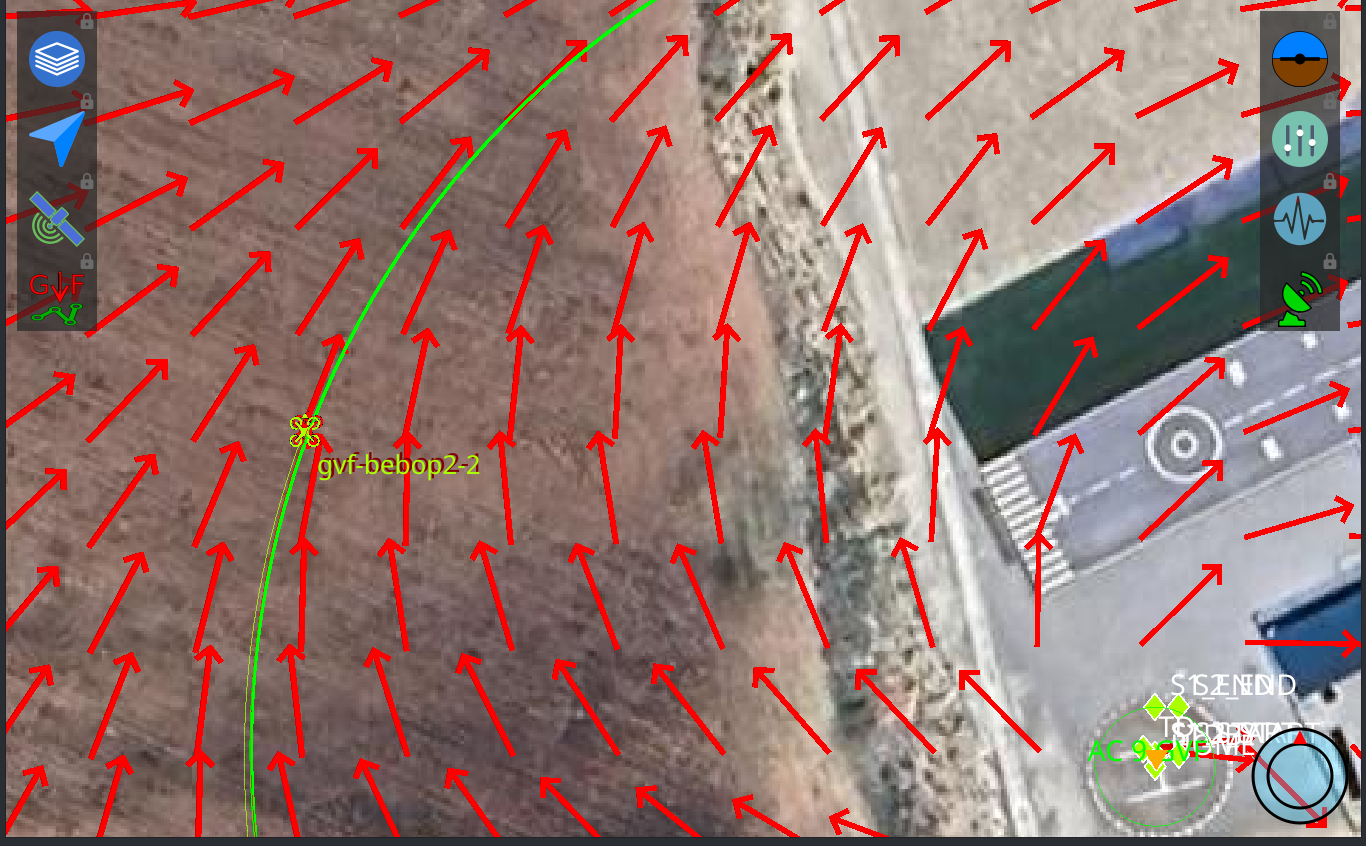
\includegraphics[width=0.99\textwidth]{img/fig/fig4.3-circular-formation-simulation-sample.png}
    \caption{Ejemplo de simulación de formaciones circulares con drones. 
    Se solapan ambos drones, al estar (como se desea) a 0 grados de error entre ambos}
    \label{fig:circular-formation-simulation}
\end{figure}

Además el error del ángulo a lo largo del tiempo ha sido el siguiente. 
Se parte de ambos haciendo GVF en un radio de unos 80 metros, con un error inicial entre ángulos de unos -6 grados sexagesimales:

\begin{figure}[h]
    \centering
    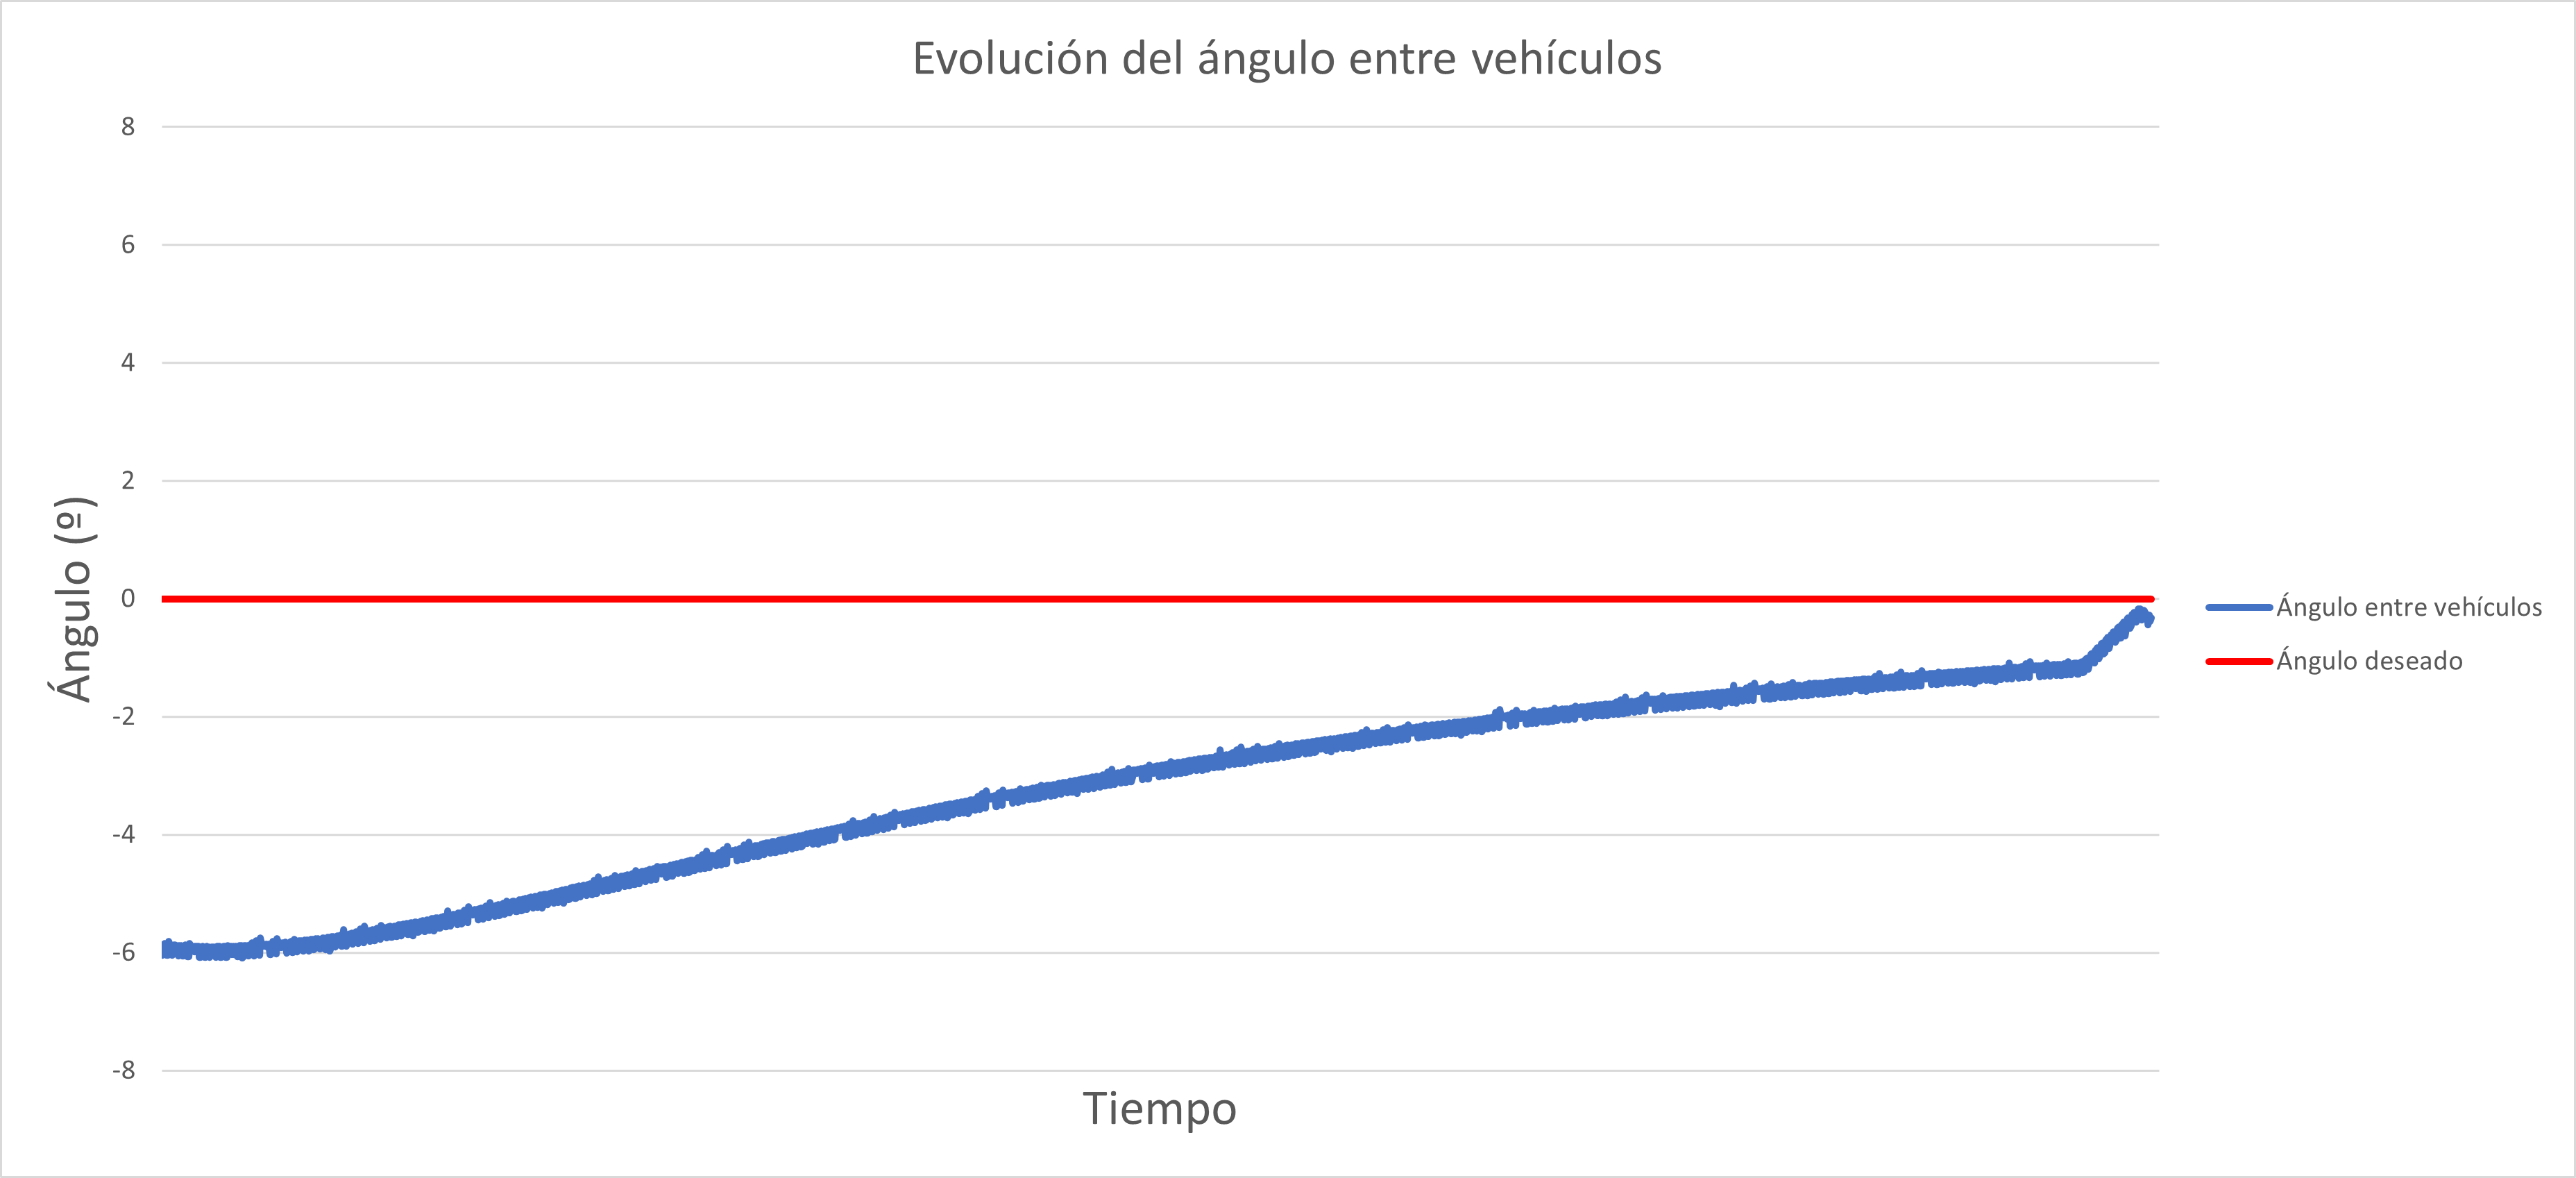
\includegraphics[width=0.99\textwidth]{img/fig/fig4.4-circular-formation-graph-error.png}
    \caption{Ángulo entre drones en simulación de formación circular. 
    En \textcolor{red}{rojo} el ángulo entre drones deseado}
    \label{fig:circular-formation-graph-error}
\end{figure}

Cómo podemos ver, converge lentamente a cerca de 0 grados de error.
No se termina de llegar a 0 ya que tomaría mucho tiempo, debido a que $k$ es aparentemente bajo para este escenario.

Tras esto, se mantiene estable en aproximadamente $\pm 1^o$ sexagesimales de error entre ambos drones.

%%%%%%%%%%%%%%%%%%%%%%%%%%%%%%%%%%%%%%%%%%%%%%%%%%%%%%%%%%%%%%%%%%%%%%%%%%%%%%%%%%%%%%%%%%%%%%%%%%%%%%%%%%%%%%%%%
%%%%%%%%%%%%%%%%%%%%%%%%%%%%%%%%%%%%%%%%%%%%%%%%%%%%%%%%%%%%%%%%%%%%%%%%%%%%%%%%%%%%%%%%%%%%%%%%%%%%%%%%%%%%%%%%%
%%%%%%%%%%%%%%%%%%%%%%%%%%%%%%%%%%%%%%%%%%%%%%%%%%%%%%%%%%%%%%%%%%%%%%%%%%%%%%%%%%%%%%%%%%%%%%%%%%%%%%%%%%%%%%%%%

\subsection{Simulación de formaciones en segmentos}

Se ha utilizado el siguiente archivo JSON:

\begin{lstlisting}[style=CodigoC]
{
  "ids": [8,9],
  "desired_normalized_offset": [0],
  "nominal_speed": 0.25,
  "gain": 0.18
}
\end{lstlisting}

Y se ha lanzado el script con los siguientes parámetros:

\begin{lstlisting}[style=CodigoBash]
python segmentFormation.py formation/segment/segment_two_bebops.json -v
\end{lstlisting}

En esta captura podemos ver dos drones en segmentos paralelos coordinados a la misma distancia en el segmento, es decir, sobre el mismo punto normalizado dentro del segmento (aproximadamente sobre 0.1):

\begin{figure}[!h]
    \centering
    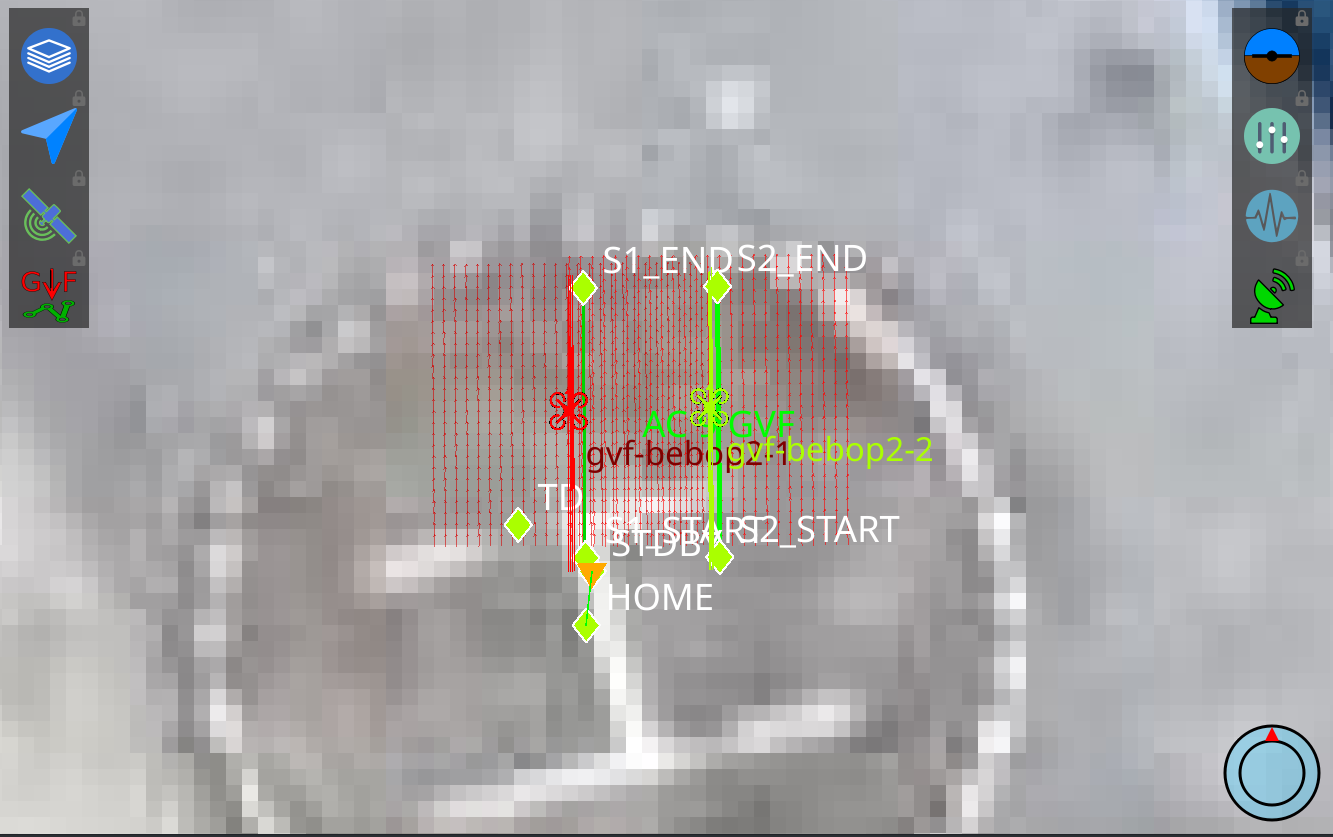
\includegraphics[width=\textwidth]{img/fig/fig4.5-segment-formation-sim.png}
    \caption{Simulación de formación en segmentos en Paparazzi. 
    Podemos ver los drones que están al lado y en paralelo}
    \label{fig:segment-formation-simulation}
\end{figure}

Además el error en la posición del segmento normalizado a lo largo del tiempo ha sido la siguiente.
Se parte de ambos haciendo GVF para segmentos con un desajuste inicial aproximado de entre -0.5 y 0.5 (según instante de tiempo):

\begin{figure}[!h]
    \centering
    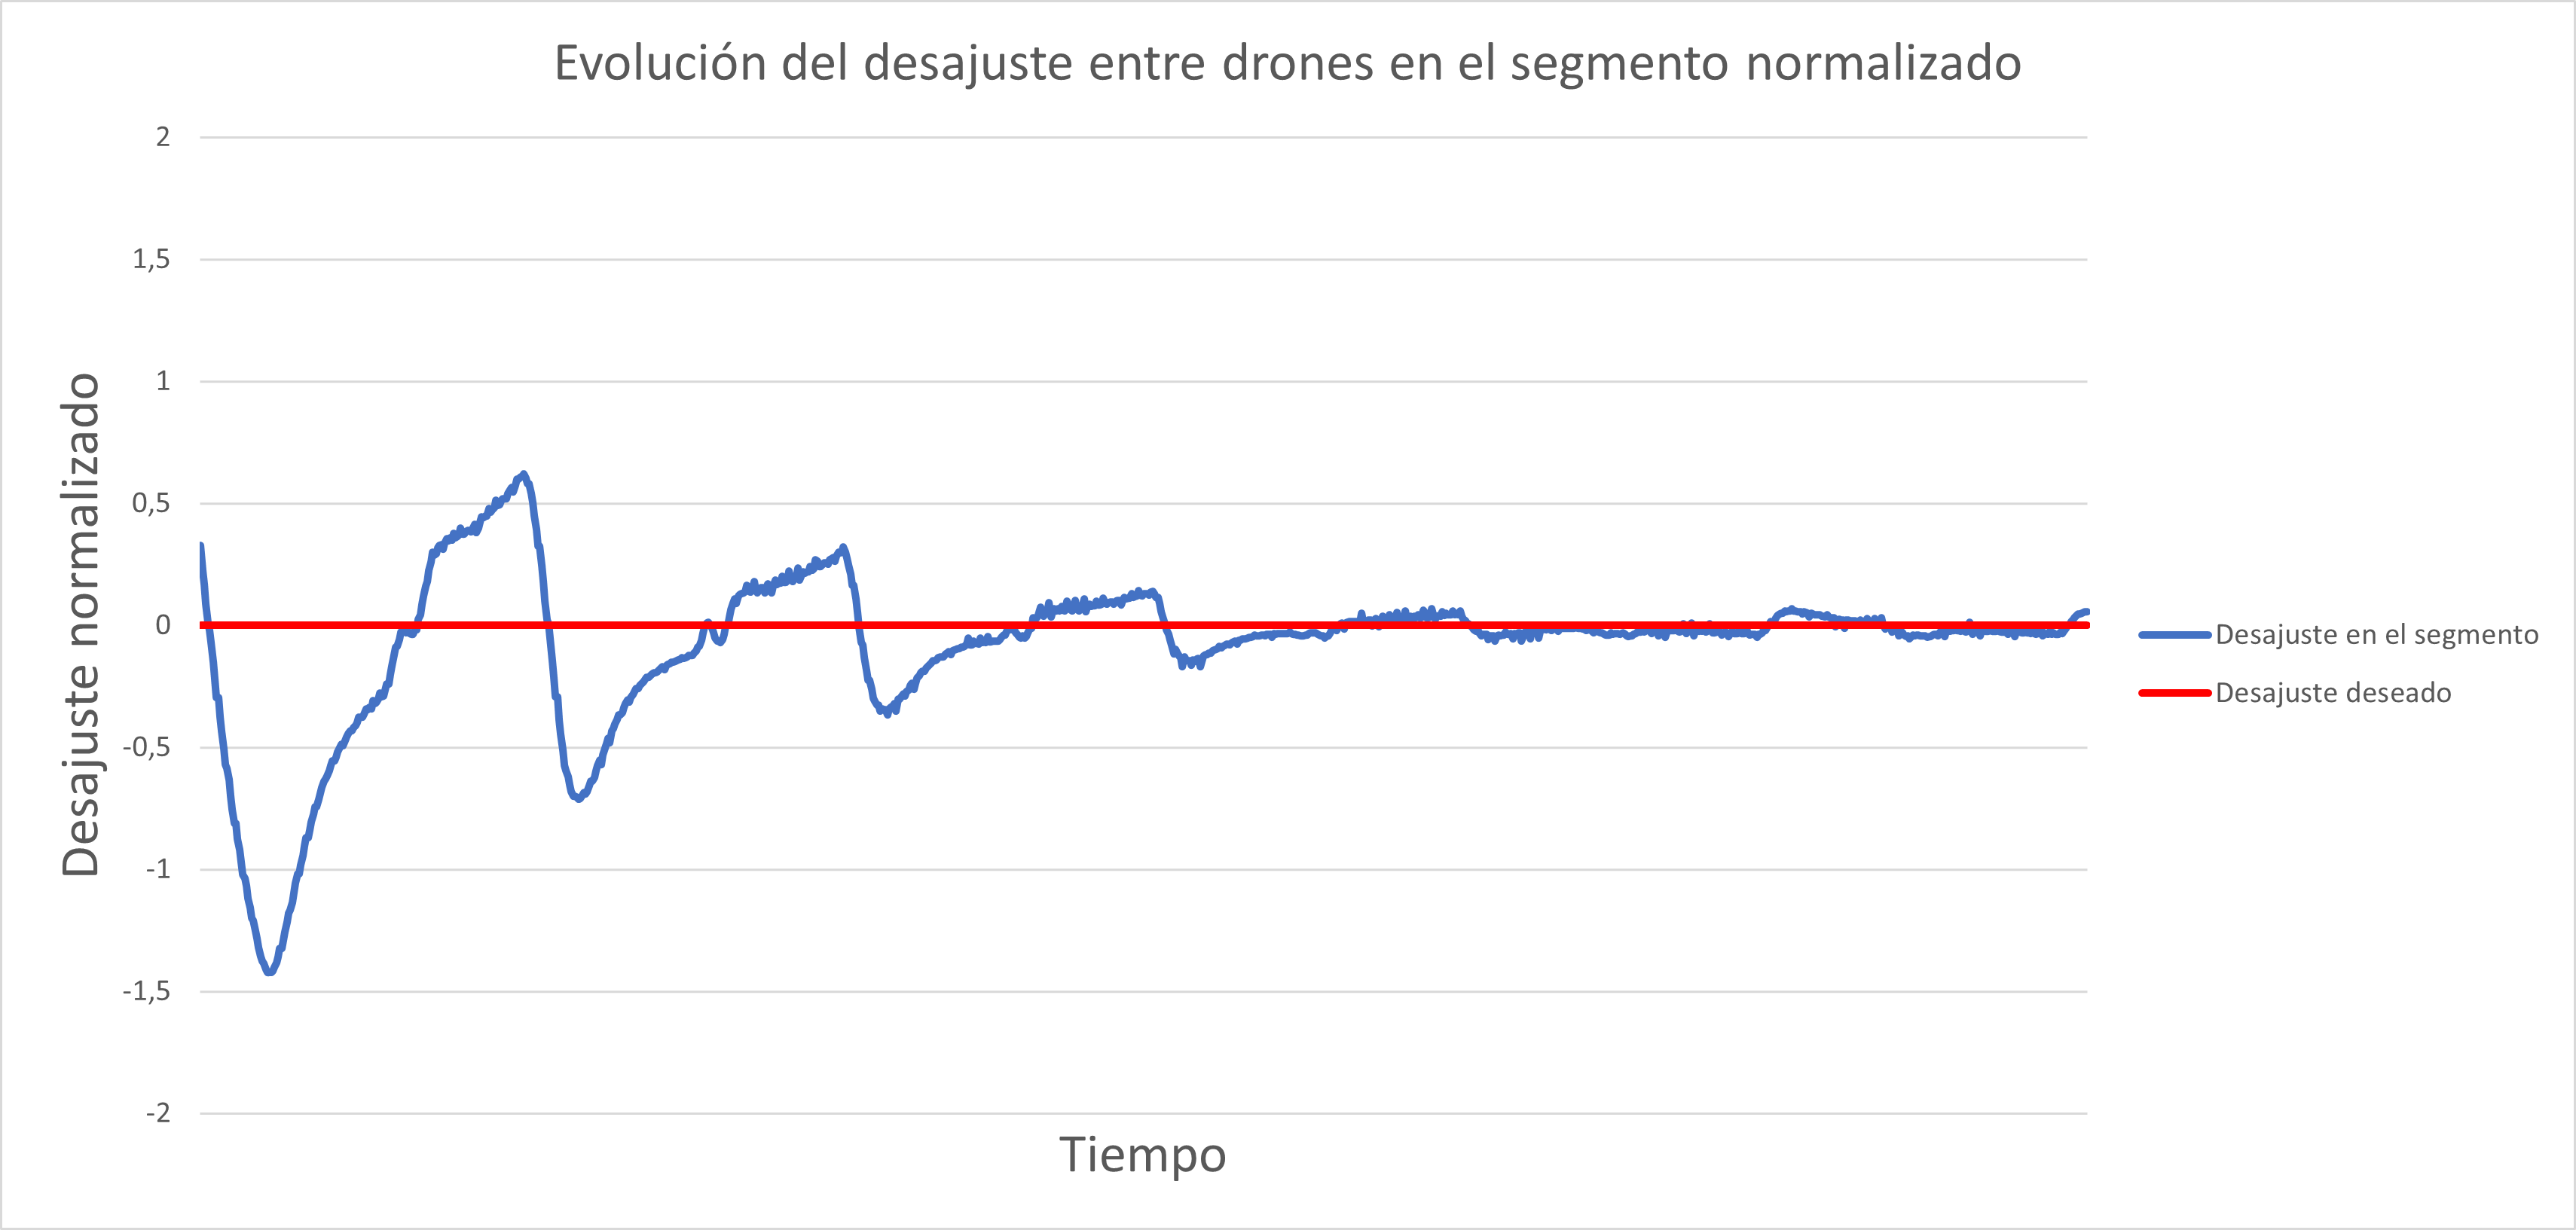
\includegraphics[width=\textwidth]{img/fig/fig4.6-segment-formation-graph-error.png}
    \caption{Desajuste de la posición sobre el segmento normalizado entre drones en simulación. En \textcolor{red}{rojo} el desajuste deseado}
    \label{fig:segment-formation-graph-error}
\end{figure}

Similarmente a formaciones circulares se converge lentamente a 0 de error, 
es decir, que uno este al lado del otro. Tras estabilizarse, el error no suele superar los $\pm 0.05$ sobre los segmentos normalizados, exceptuando en los extremos de los segmentos, que se suele ganar algo de error. 

%%%%%%%%%%%%%%%%%%%%%%%%%%%%%%%%%%%%%%%%%%%%%%%%%%%%%%%%%%%%%%%%%%%%%%%%%%%%%%%%%%%%%%%%%%%%%%%%%%%%%%%%%%%%%%%%%
%%%%%%%%%%%%%%%%%%%%%%%%%%%%%%%%%%%%%%%%%%%%%%%%%%%%%%%%%%%%%%%%%%%%%%%%%%%%%%%%%%%%%%%%%%%%%%%%%%%%%%%%%%%%%%%%%
%%%%%%%%%%%%%%%%%%%%%%%%%%%%%%%%%%%%%%%%%%%%%%%%%%%%%%%%%%%%%%%%%%%%%%%%%%%%%%%%%%%%%%%%%%%%%%%%%%%%%%%%%%%%%%%%%

\section{Coordinación y formación de Crazyflies}

Por último, se han de probar los experimentos de simulación en los Crazyflies reales.
Como se ha explicado previamente, se van a obviar los experimentos de formaciones circulares ya que no se dispone de un buen lugar para estos experimentos. 

%%%%%%%%%%%%%%%%%%%%%%%%%%%%%%%%%%%%%%%%%%%%%%%%%%%%%%%%%%%%%%%%%%%%%%%%%%%%%%%%%%%%%%%%%%%%%%%%%%%%%%%%%%%%%%%%%
%%%%%%%%%%%%%%%%%%%%%%%%%%%%%%%%%%%%%%%%%%%%%%%%%%%%%%%%%%%%%%%%%%%%%%%%%%%%%%%%%%%%%%%%%%%%%%%%%%%%%%%%%%%%%%%%%
%%%%%%%%%%%%%%%%%%%%%%%%%%%%%%%%%%%%%%%%%%%%%%%%%%%%%%%%%%%%%%%%%%%%%%%%%%%%%%%%%%%%%%%%%%%%%%%%%%%%%%%%%%%%%%%%%

\subsection{Comparación entre firmware oficial y de Paparazzi}

Las primeras pruebas resultaron ser prometedoras, pero no suficiente, ya que el Flow Deck, aunque mejor que la IMU sola, 
acumula suficiente error como para que antes de que se coordinen ambos drones se choquen o desvíen demasiado del objetivo, sin llegar a coordinarse. 
En otras palabras, se puede realizar GVF y/o coordinación bajo un tiempo límite si se utiliza posición relativa, 
pero la coordinación necesita más de ese tiempo límite. 
Aquí es un buen ejemplo donde el Loco Positioning System explicado en el capítulo 1 hubiese ayudado, 
pero se descartó finalmente por falta de un lugar apropiado donde instalarlo.

Consecuentemente, se probó con el firmware de Bitcraze (que se utilizó en el capítulo 2) la estabilidad a lo largo del tiempo y resultó ser considerablemente mayor. 
En otras palabras, el ajuste de estabilización del PID y lectura de los sensores es \textbf{claramente superior en el firmware oficial a en Paparazzi}. En resumen:

\begin{itemize}
    \item El firmware de Paparazzi es superior en versatilidad, opciones de módulos, telemetría... y es capaz de hacer simulaciones.
    \item Por contraparte, el firmware de Bitcraze es superior en control del Crazyflie, facilidad de uso (tanto programación como uso general) y documentación.
\end{itemize}

Por ello, tras demostrar la viabilidad del algoritmo en simulación, se va a realizar la demostración de la coordinación \textbf{bajo el firmware oficial de Bitcraze}.

%%%%%%%%%%%%%%%%%%%%%%%%%%%%%%%%%%%%%%%%%%%%%%%%%%%%%%%%%%%%%%%%%%%%%%%%%%%%%%%%%%%%%%%%%%%%%%%%%%%%%%%%%%%%%%%%%
%%%%%%%%%%%%%%%%%%%%%%%%%%%%%%%%%%%%%%%%%%%%%%%%%%%%%%%%%%%%%%%%%%%%%%%%%%%%%%%%%%%%%%%%%%%%%%%%%%%%%%%%%%%%%%%%%
%%%%%%%%%%%%%%%%%%%%%%%%%%%%%%%%%%%%%%%%%%%%%%%%%%%%%%%%%%%%%%%%%%%%%%%%%%%%%%%%%%%%%%%%%%%%%%%%%%%%%%%%%%%%%%%%%

\subsection{Control en el firmware de Bitcraze}

Para entender mejor esta subsección y las siguientes,
se recomienda leer paralelamente el \autoref{appendix:user_manual},
concretamente la sección para Bitcraze. Veamos un script de ejemplo:

\begin{lstlisting}[style=CodigoPython]
# crazyflie_demo.py
# ...

import cflib.crtp
from cflib.crazyflie import Crazyflie
from cflib.crazyflie.syncCrazyflie import SyncCrazyflie
from cflib.positioning.motion_commander import MotionCommander
from cflib.utils import uri_helper

URI = uri_helper.uri_from_env(default='radio://0/80/2M/E7E7E7E701')
DEFAULT_HEIGHT = 0.5

# ...

def move_linear_simple(scf):
    with MotionCommander(scf, default_height=DEFAULT_HEIGHT) as mc:
        time.sleep(1)
        mc.forward(0.5)
        time.sleep(1)
        mc.turn_left(180)
        time.sleep(1)
        mc.forward(0.5)
        time.sleep(1)

# ...

if __name__ == '__main__':
    cflib.crtp.init_drivers()

    with SyncCrazyflie(URI, cf=Crazyflie(rw_cache='./cache')) as scf:
        # ...
        move_linear_simple(scf)
\end{lstlisting}

\textbf{\texttt{\# ...} representa fragmentos de código que no se han escrito} 
porque no son necesarios para entender la totalidad del código.

Cómo podemos ver en el fragmento de código anterior, 
el control de un Crazyflie es trivial en comparación con Paparazzi.
El ajuste de PID, los diversos módulos, la necesidad de recompilar el firmware...
todo esta abstraído de forma que pueda ser más simple el control básico.

A grandes rasgos, tan sólo hay que inicializar los drivers, 
crear el objeto \texttt{scf} para control del Crazyflie y llamar a una función que indica que se va a comandar.
En la función tan sólo hay que indicar si se quiere ir hacia delante, atrás, rotar...
Por supuesto existen otros métodos de control, por ejemplo, dirigirse hacia cierta posición, o comandar
directamente el roll, pitch, yaw y throttle.

%%%%%%%%%%%%%%%%%%%%%%%%%%%%%%%%%%%%%%%%%%%%%%%%%%%%%%%%%%%%%%%%%%%%%%%%%%%%%%%%%%%%%%%%%%%%%%%%%%%%%%%%%%%%%%%%%
%%%%%%%%%%%%%%%%%%%%%%%%%%%%%%%%%%%%%%%%%%%%%%%%%%%%%%%%%%%%%%%%%%%%%%%%%%%%%%%%%%%%%%%%%%%%%%%%%%%%%%%%%%%%%%%%%
%%%%%%%%%%%%%%%%%%%%%%%%%%%%%%%%%%%%%%%%%%%%%%%%%%%%%%%%%%%%%%%%%%%%%%%%%%%%%%%%%%%%%%%%%%%%%%%%%%%%%%%%%%%%%%%%%

\subsection{Formación en segmentos en el firmware de Bitcraze}

Para implementar el algoritmo de coordinación sobre el firmware oficial, 
se ha decidio obviar GVF ya que, aunque es preferible debido al buen control que ofrece,
no es necesario para hacer una demostración del algoritmo de coordinación.
Por ello la implementación de la coordinación en segmentos se ha realizado de la siguiente forma \cite{crazyradio-swarm-interface}:

\begin{lstlisting}[style=CodigoPython]
# crazyflie_segment_formation.py
# ...

uris = {
    'radio://0/80/2M/E7E7E7E701',
    'radio://0/80/2M/E7E7E7E702',
}

waiting_uri = 'radio://0/80/2M/E7E7E7E702' # Crazyflie that waits
all_positions = {}

NOMINAL_SPEED = [0.2, 0] # x, y respectively
DEFAULT_HEIGHT = 0.5 # In meters
SEGMENT_LIMIT = 1 # Meters
FREQ = 0.2 # How many seconds until we update the speed

# ...

def kuramoto(my_position, other_positions):
    k = 0.12
    desired_offset = 0

    delta = 0
    for position in other_positions:
        delta += position[0] - my_position[0] - desired_offset
    
    return k * delta

def get_xy_from(radio, positions):
    return (positions[radio].x, positions[radio].y)
    
def coordinated_segment(scf):
    with MotionCommander(scf, default_height=DEFAULT_HEIGHT) as mc:
        my_nominal_speed = {}
        my_nominal_speed[scf._link_uri] = NOMINAL_SPEED
        
        # ...

        while True:
            # First we calculate positions
            my_position = get_xy_from(scf._link_uri, all_positions)

            # Calculate every other drone position
            other_positions = []
            for uri in uris:
                if uri != scf._link_uri:
                    other_positions.append(get_xy_from(uri, all_positions))

            # Change direction if passed the limit
            if my_position[0] > SEGMENT_LIMIT:
                my_nominal_speed[scf._link_uri][0] = -NOMINAL_SPEED[0]
            elif my_position[0] < -SEGMENT_LIMIT:
                my_nominal_speed[scf._link_uri][0] = NOMINAL_SPEED[0]

            speed_x = my_nominal_speed[scf._link_uri][0]
            
            # Add Kuramoto speed
            speed_x += kuramoto(my_position, other_positions)

            mc.start_linear_motion(speed_x, speed_y, 0)
            time.sleep(FREQ)

def recover_positions():
    global all_positions
    while True:
        all_positions = swarm.get_estimated_positions()
        time.sleep(FREQ / 2)

if __name__ == '__main__':
    # ...
    with Swarm(uris, factory=factory) as swarm:        
        # ...
        recover_positions_thread.start()
        swarm.parallel(coordinated_segment)
        # ...
\end{lstlisting}

Similarmente al ejemplo anterior, \textbf{\texttt{\# ...} representa trozos de código que se han obviado} al no ser
relevantes para entender la funcionalidad principal.

Podemos dividir el código en las siguientes secciones:

\begin{itemize}
    \item \texttt{recover\_positions()}: función que se ocupa de recuperar las posiciones de los drones 
    cada \texttt{FREQ / 2} segundos. Se ejecuta en un thread aparte.
    \item \texttt{kuramoto()}: recibe las posiciones de todos los drones y calcula para cada dron cuanto debe
    aumentar o reducir su velocidad con el algoritmo para segmentos paralelos.
    \item \texttt{coordinated\_segment():} función principal para coordinar los drones.
    Calcula posiciones, invierte la velocidad lineal de un dron si ha pasado del segmento y 
    comanda la velocidad calculada por el algoritmo cada \texttt{FREQ} segundos.
\end{itemize}

En general, esta implementación simplificada sigue un segmento en X sin importar su posición en Y.
Su dirección cambiará cuando llegue a 1 metro y cuando llegue a -1 metro, permitiendo obviar la normalización.
Si bien puede ser simple, el objetivo final que es aplicar el algoritmo, se puede conseguir igualmente.

%%%%%%%%%%%%%%%%%%%%%%%%%%%%%%%%%%%%%%%%%%%%%%%%%%%%%%%%%%%%%%%%%%%%%%%%%%%%%%%%%%%%%%%%%%%%%%%%%%%%%%%%%%%%%%%%%
%%%%%%%%%%%%%%%%%%%%%%%%%%%%%%%%%%%%%%%%%%%%%%%%%%%%%%%%%%%%%%%%%%%%%%%%%%%%%%%%%%%%%%%%%%%%%%%%%%%%%%%%%%%%%%%%%
%%%%%%%%%%%%%%%%%%%%%%%%%%%%%%%%%%%%%%%%%%%%%%%%%%%%%%%%%%%%%%%%%%%%%%%%%%%%%%%%%%%%%%%%%%%%%%%%%%%%%%%%%%%%%%%%%

\subsection{Resultados de la coordinación}

Ejecutando el programa mostrado en la subsección anterior, los resultados fueron prometedores: 
el algoritmo funciona correctamente, pero actualmente hay un error en el código de Bitcraze que impiden que se den la vuelta correctamente en el segmento.

\begin{figure}[h]
    \centering
    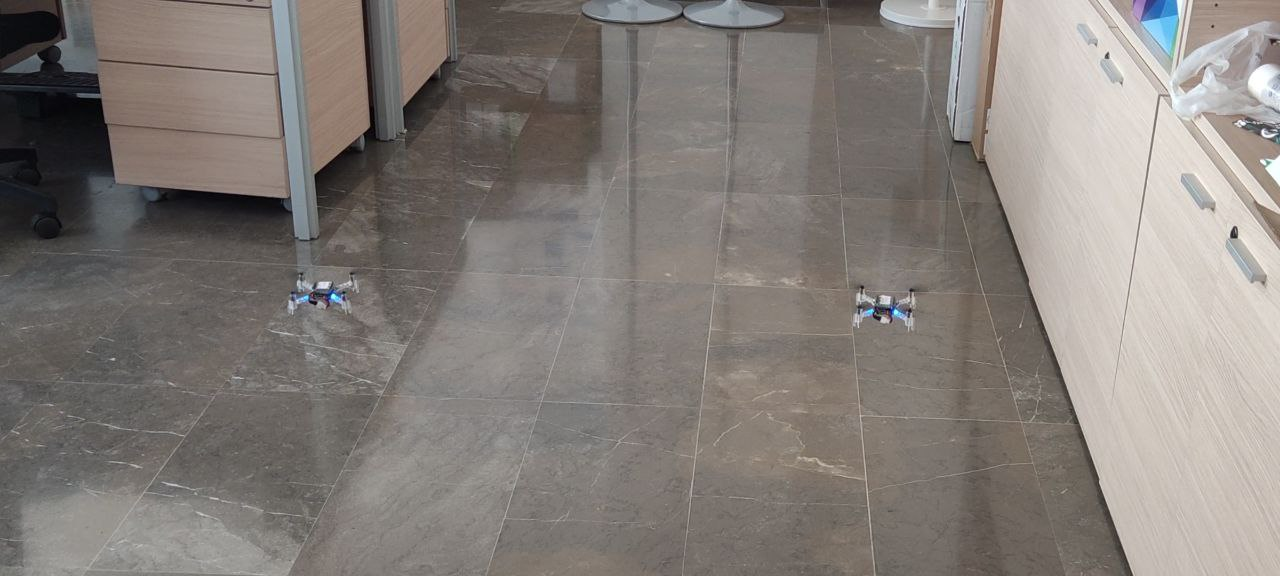
\includegraphics[width=\textwidth]{img/fig/fig4.7-coordinated-crazyflies.jpg}
    \caption{Dos drones manteniéndose paralelos. 
    En este caso $p^* = 0, \ v_n = 0.2 \ m/s, \ K = 0.12$}
    \label{fig:coordinated-crazyflies}
\end{figure}

Para verificar que esto no es culpa de un error en la programación o algoritmo,
se ha decidido añadir un último experimento que utiliza un log real de un sólo dron siguiendo un segmento y 
un dron simulado aplicando el algoritmo en base a las posiciones reales del log, 
es decir, tratando de mantenerse coordinado con las posiciones del dron real guardadas en el log.
Mas información de este experimento en el \autoref{appendix:user_manual}.

Para este experimento:

\begin{itemize}
    \item $p^* = 0, \ v_n = 0.1 \ m/s$. 
    Para el caso del log sacado del dron real, se mantuvo una velocidad fija de $0.1 \ m/s$.
    \item Se fijo un segmento con posiciones $(-0.5, 0)$ y $(0.5, 0)$, es decir,
    para este caso no se normalizó el segmento. 
    Consecuentemente,  se ha decidido que $K = 0.3$ (3 veces más alto que la velocidad nominal), 
    para compensar por el hecho de que el segmento es más corto. 
    \item También, se ha elegido un valor de $K$ más alto para que se pueda mantener más cerca el dron simulado del real, ya que al ser una simulación controlado se pueden evitar los posibles errores de elegir un $K$ alto.
    \item Por último, se ha decidido fijar las posiciones en el eje Y. 
    En el caso del dron real hubo una ligera variación, pero por simplificar, se ha asumido que los valores de $p_y$ fueron constantes.
\end{itemize}

\begin{figure}[h]
    \centering
    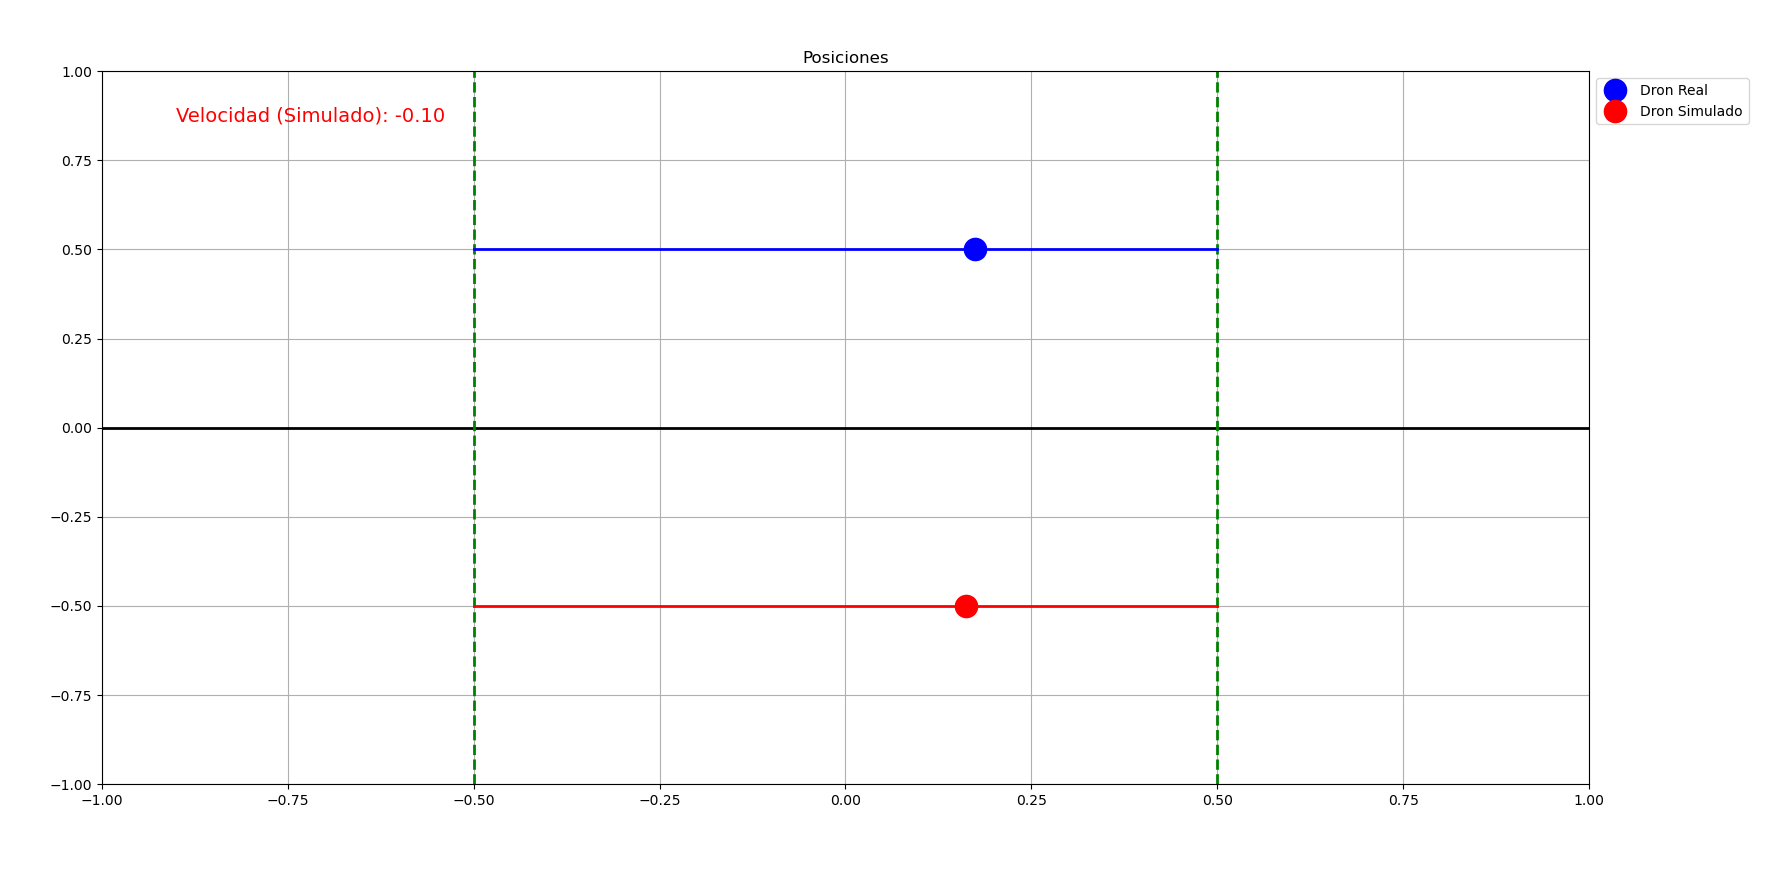
\includegraphics[width=\textwidth]{img/fig/fig4.8-coordinated-experiment.png}
    \caption{Animación del experimento que verifica que el algoritmo funciona}
    \label{fig:coordination-experiment}
\end{figure}

En la siguiente figura podemos ver el error de la posición entre los drones. 
Se obvian los dos primeros segundos que el dron simulado esta quieto:

\begin{figure}[h]
    \centering
    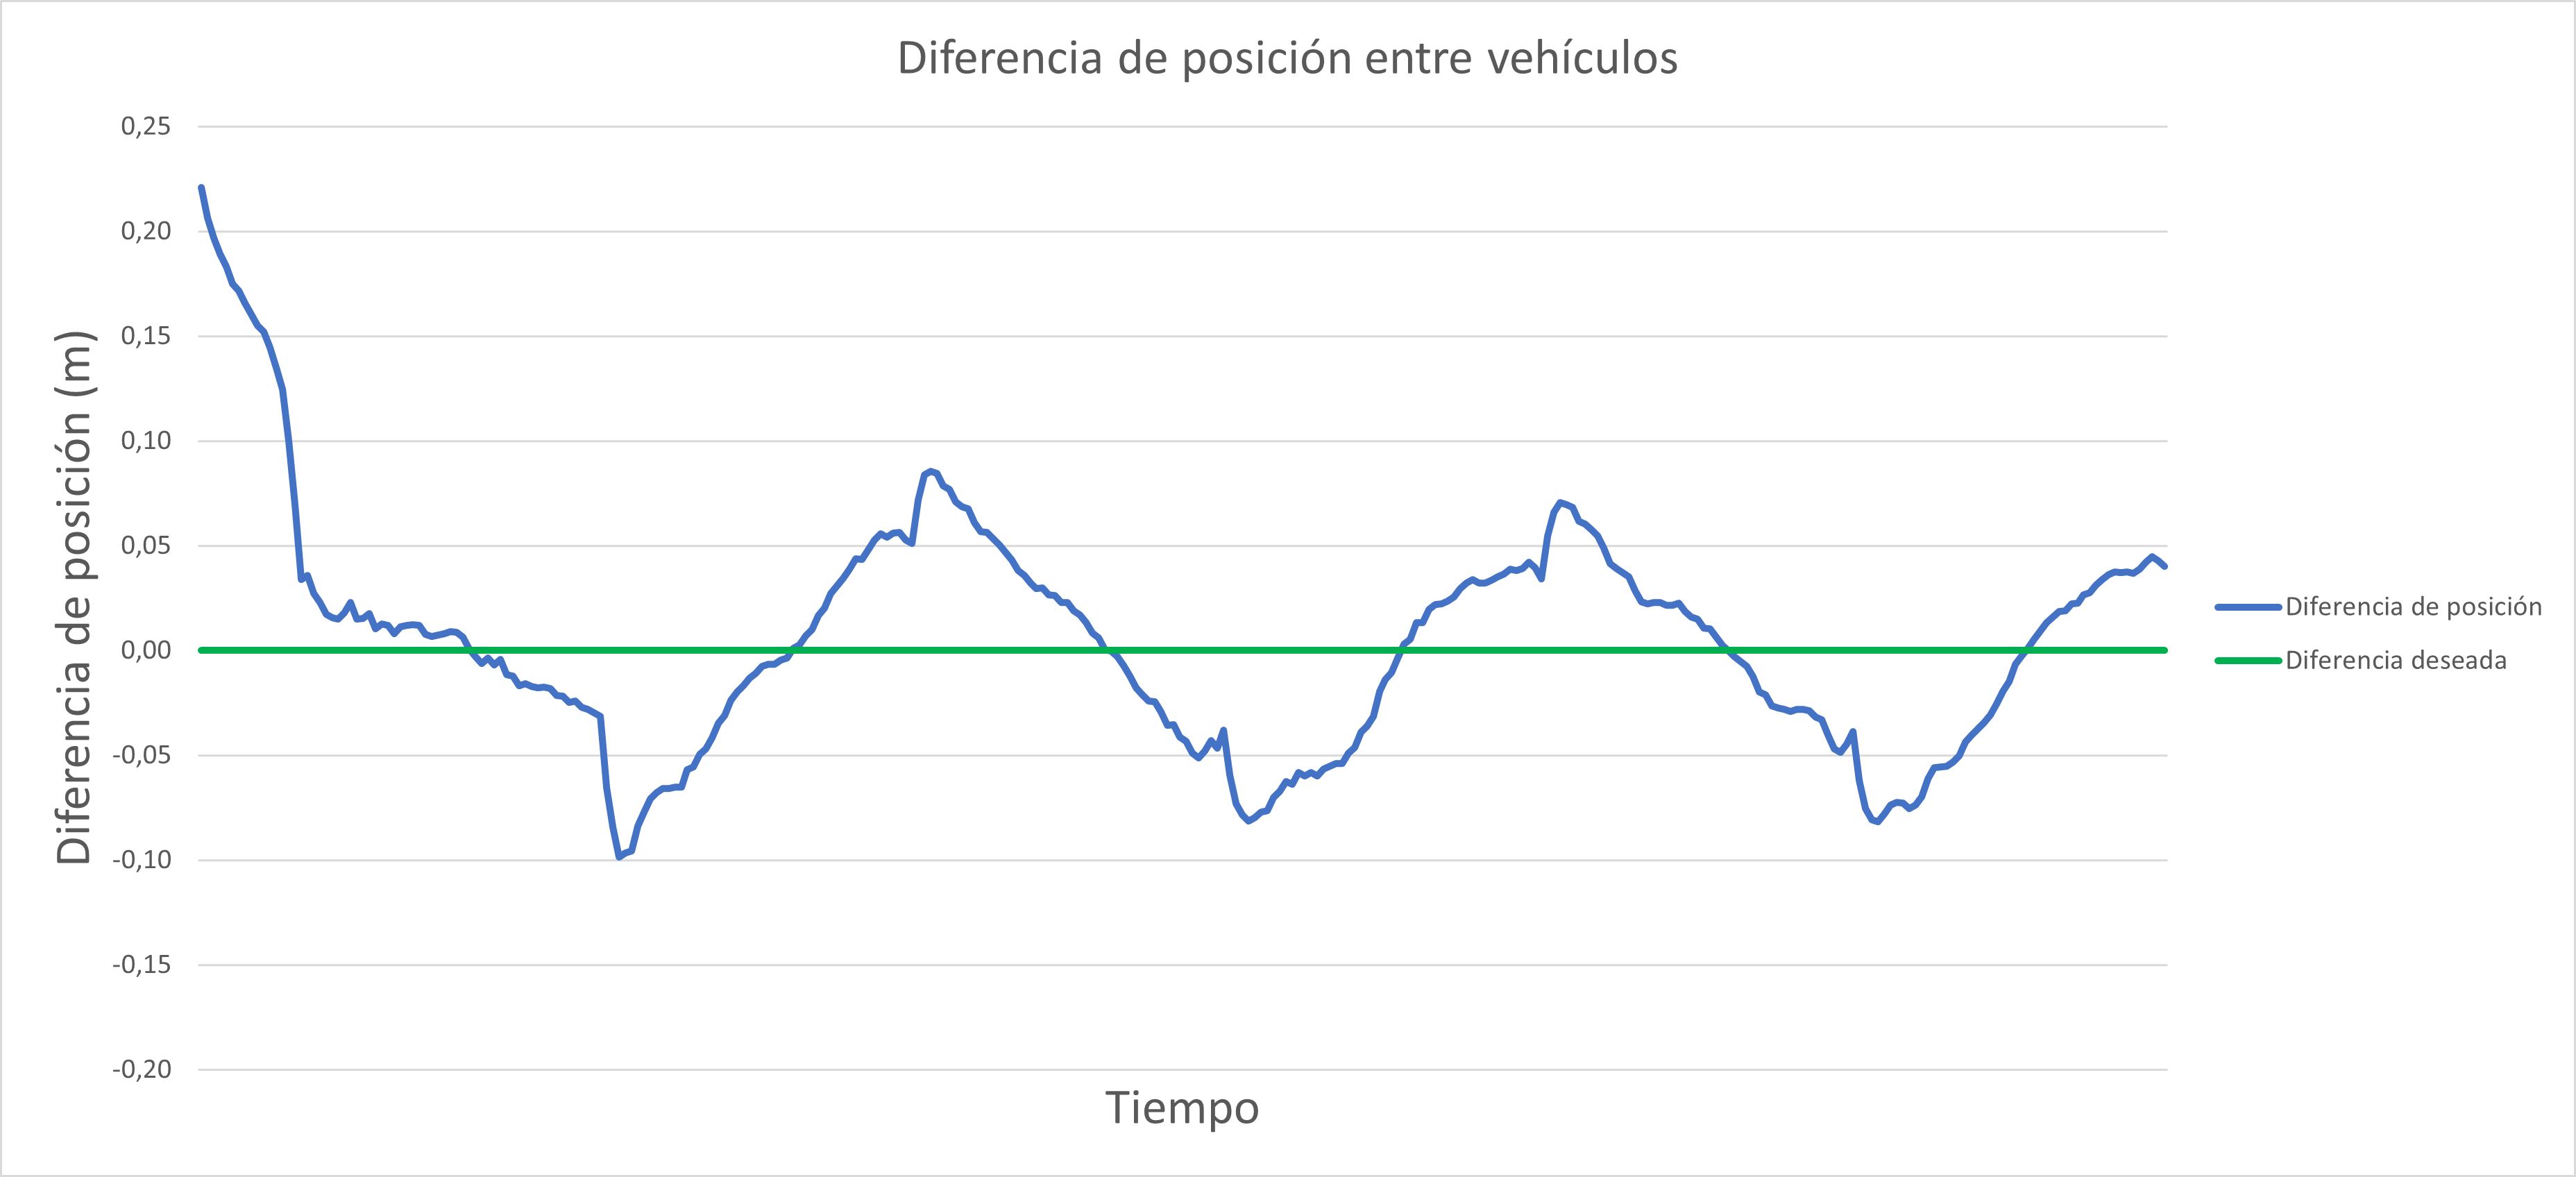
\includegraphics[width=\textwidth]{img/fig/fig4.9-experiment-pos-error.png}
    \caption{Diferencia de la posición entre los drones. 
    En \textcolor{Green3}{verde} la diferencia deseado}
    \label{fig:pos-error-experiment}
\end{figure}

Podemos ver que el error no sube de 0.1 m tras estabilizarse.
Si obviamos los máximos locales (se producen al dar la vuelta en el segmento), el error esta típicamente por debajo de 0.05 m, es decir por debajo del $10\%$ de error.

Por último, la velocidad del dron simulado fue la siguiente (para los mismos instantes de tiempo):

\begin{figure}[h]
    \centering
    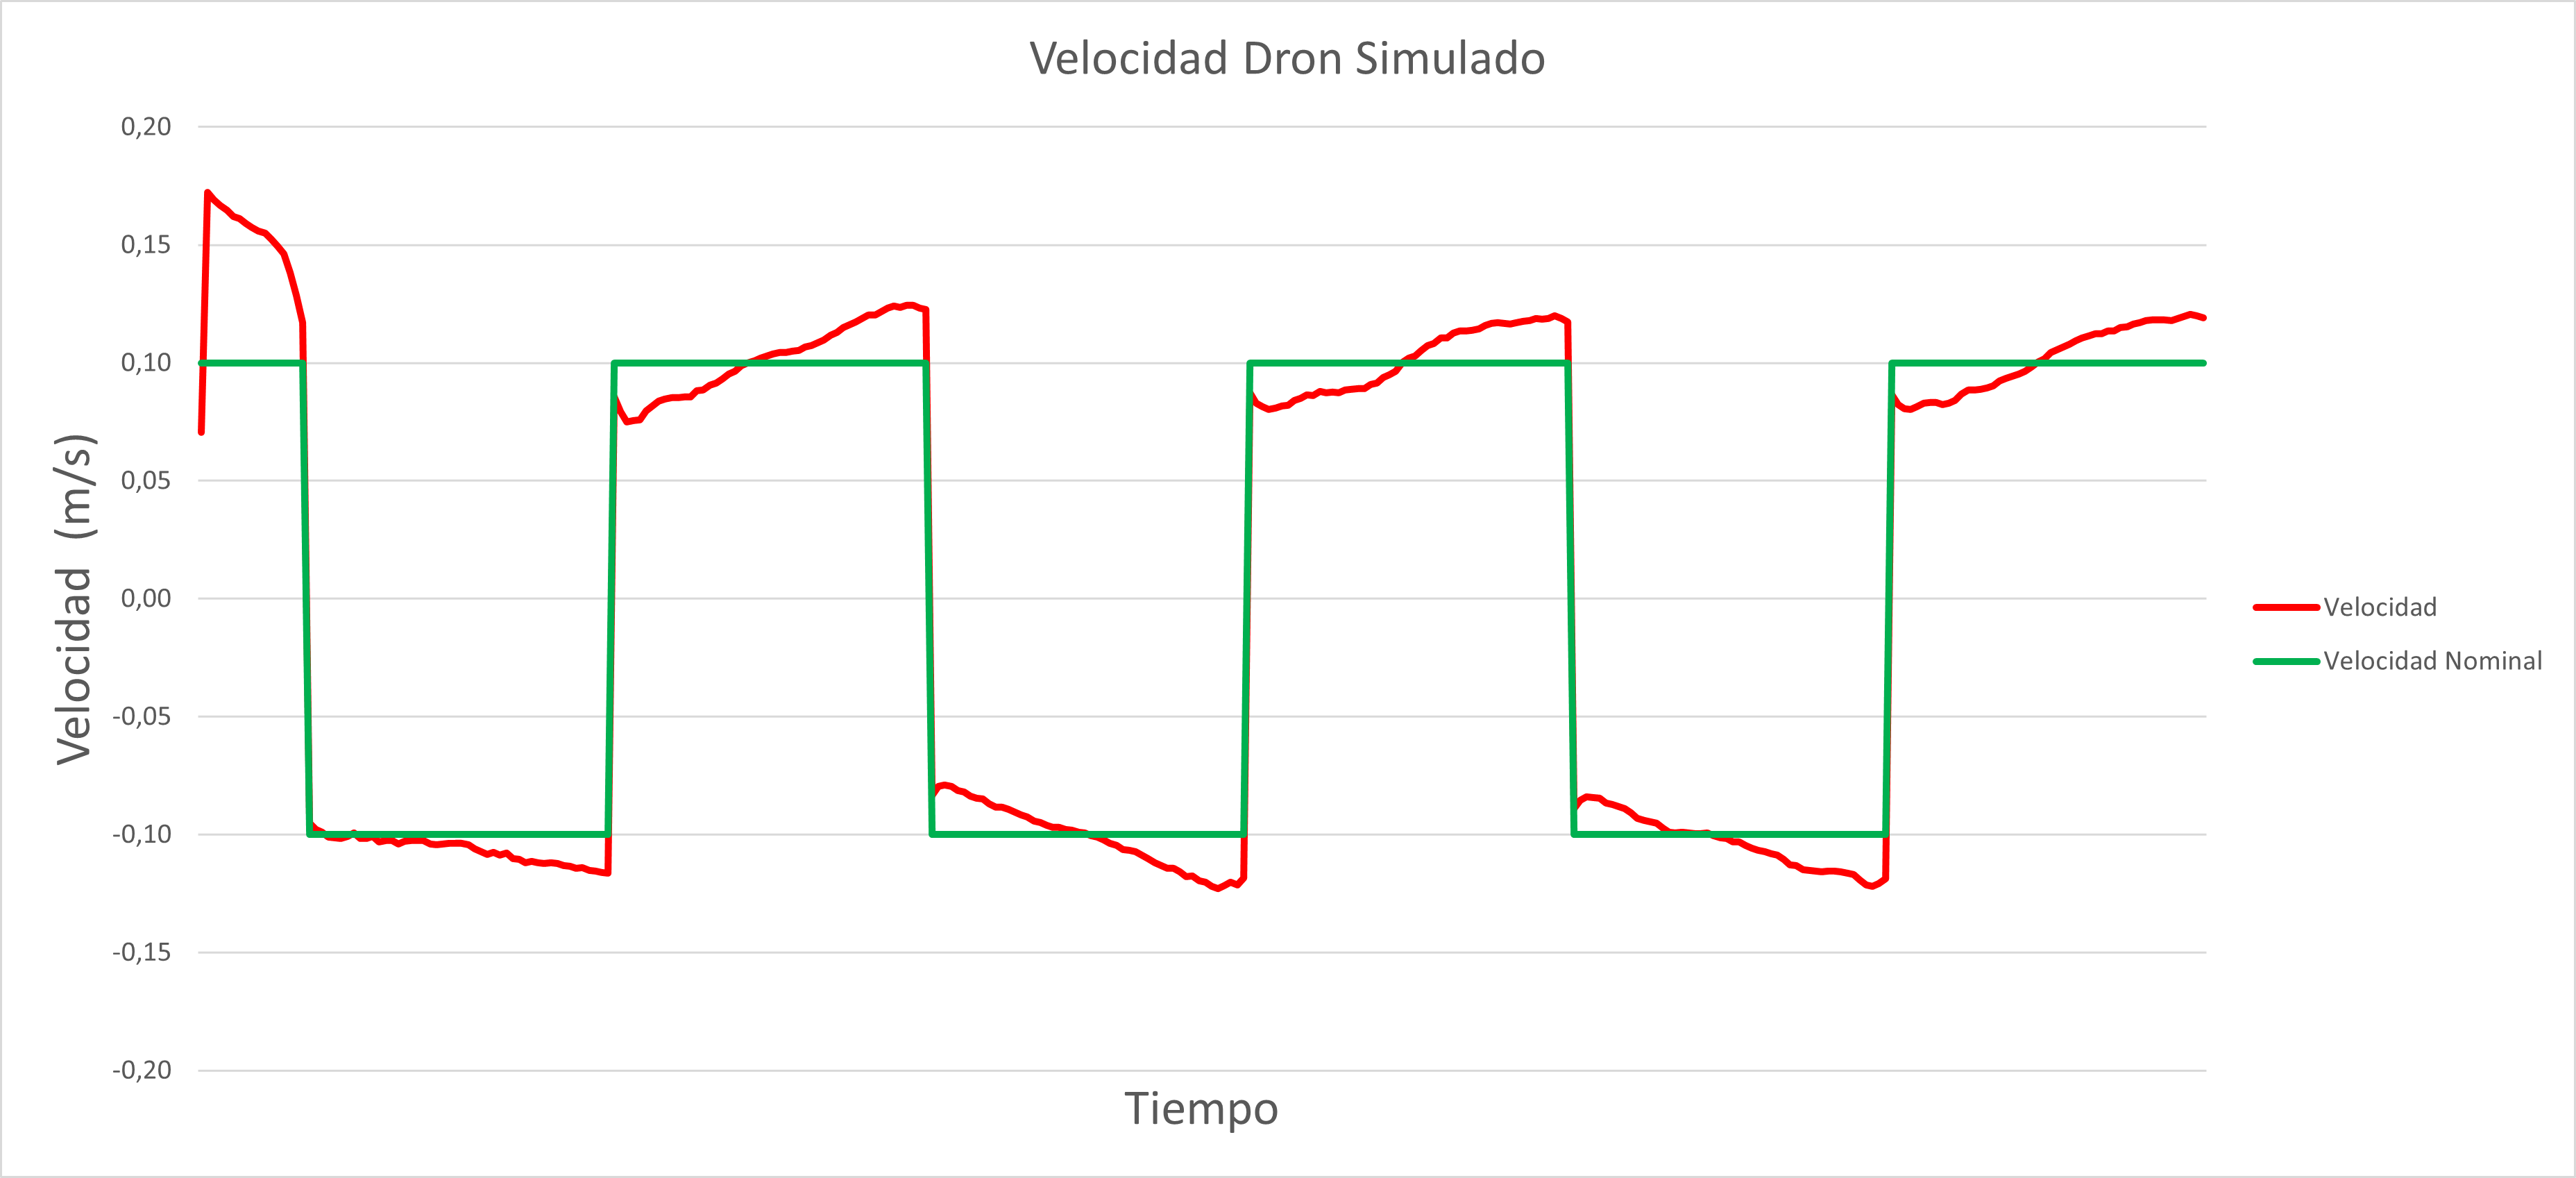
\includegraphics[width=\textwidth]{img/fig/fig4.10-experiment-speed.png}
    \caption{Velocidad del dron rojo (simulado). 
    En \textcolor{Green3}{verde} la velocidad nominal objetivo en ese instante}
    \label{fig:speed-experiment}
\end{figure}

Es interesante ver los bruscos cambios, al ser un dron simulado sin GVF.

Este experimento también sirve para entender las impresionantes capacidades de Paparazzi para simulación.
Es evidente que para ello, Paparazzi es superior a otras alternativas software,
en especial para los Crazyflies, que no dispone de una extensa variedad.

Finalmente, se recomienda para ambos experimentos ver las animaciones y vídeos correspondientes en la presentación por diapositivas de este TFG para entender mejor los resultados que en las figuras \cite{final-results}. 
    \chapter{Conclusiones}

En este último capítulo, se extraen conclusiones en base a los resultados obtenidos.
Se incluye, por supuesto, un análisis de los objetivos y planificación, asi como posibles aplicaciones,
para poder extraer conclusiones desde un punto de vista de la ingeniería en general, 
además de los resultados mas tangibles y observables a simple vista.

%%%%%%%%%%%%%%%%%%%%%%%%%%%%%%%%%%%%%%%%%%%%%%%%%%%%%%%%%%%%%%%%%%%%%%%%%%%%%%%%%%%%%%%%%%%%%%%%%%%%%%%%%%%%%%%%%
%%%%%%%%%%%%%%%%%%%%%%%%%%%%%%%%%%%%%%%%%%%%%%%%%%%%%%%%%%%%%%%%%%%%%%%%%%%%%%%%%%%%%%%%%%%%%%%%%%%%%%%%%%%%%%%%%
%%%%%%%%%%%%%%%%%%%%%%%%%%%%%%%%%%%%%%%%%%%%%%%%%%%%%%%%%%%%%%%%%%%%%%%%%%%%%%%%%%%%%%%%%%%%%%%%%%%%%%%%%%%%%%%%%

\section{Análisis de los objetivos y planificación}

Es importante observar hasta que punto se cumplieron las metas establecidas. 
Por ello, a continuación se muestra un pequeño análisis de si se cumplió cada objetivo, 
y hasta que punto:

\begin{itemize}
    \item \textbf{OBJ-1:} introducción, objetivos, planificación y preparación general. 
    Es evidente que se cumplió este objetivo, al ser introductorio y de carácter anterior al resto de objetivos.
    
    \item \textbf{Capítulo 2 (OBJ-2):} preliminares. 
    Se cumplió perfectamente este objetivo. No obstante,
    hubo ciertos retrasos que veremos en la siguiente subsección de planificación.

    \item \textbf{Capítulo 3 (OBJ-3):} control de un Crazyflie. 
    Se consiguió implementar el control de un Crazyflie en Paparazzi, tanto en simulación como en la realidad. 
    El único problema fue que el control en movimiento en Paparazzi fue peor a lo esperado.
    
    \item \textbf{Capítulo 4 (OBJ-4):} coordinación entre Crazyflies. 
    Se consiguió este objetivo plenamente, los resultados finales han sido prometedores y se ha utilizado tanto Paparazzi como el software y firmware oficial. 
    La única diferencia es que no se pudo conseguir control aceptable bajo Paparazzi, negando la posibilidad de intentar coordinación en este software. 

    \item \textbf{Capítulo 5 (OBJ-5):} conclusiones.
    Similar al OBJ-1, este objetivo se puede considerar evidente, al ser un objetivo que se cumple casi automáticamente al terminar el resto de objetivos.

    \item \textbf{OBJ-6:} Revisión y mejora general.
    Si bien se ha calificado como objetivo, este último es un poco más ambiguo y subjetivo de poder hacer una evaluación de su cumplimiento. 
    En general, considero personalmente que fue buena elección dedicar y planificar un tiempo a la revisión y mejora general del trabajo en su conjunto.
    En los resultados de la planificación (siguiente subsección) veremos que se decidió finalmente hacerlo en paralelo al trabajo (intercalando) y no sólo al final.
\end{itemize}

Acompañado al análisis de objetivos, para comparar si se ha realizado una buena planificación, 
se ha realizado otro diagrama de Gantt, 
que muestra como se distribuyeron los objetivos a lo largo del desarrollo:

\begin{figure}[h]
    \centering
    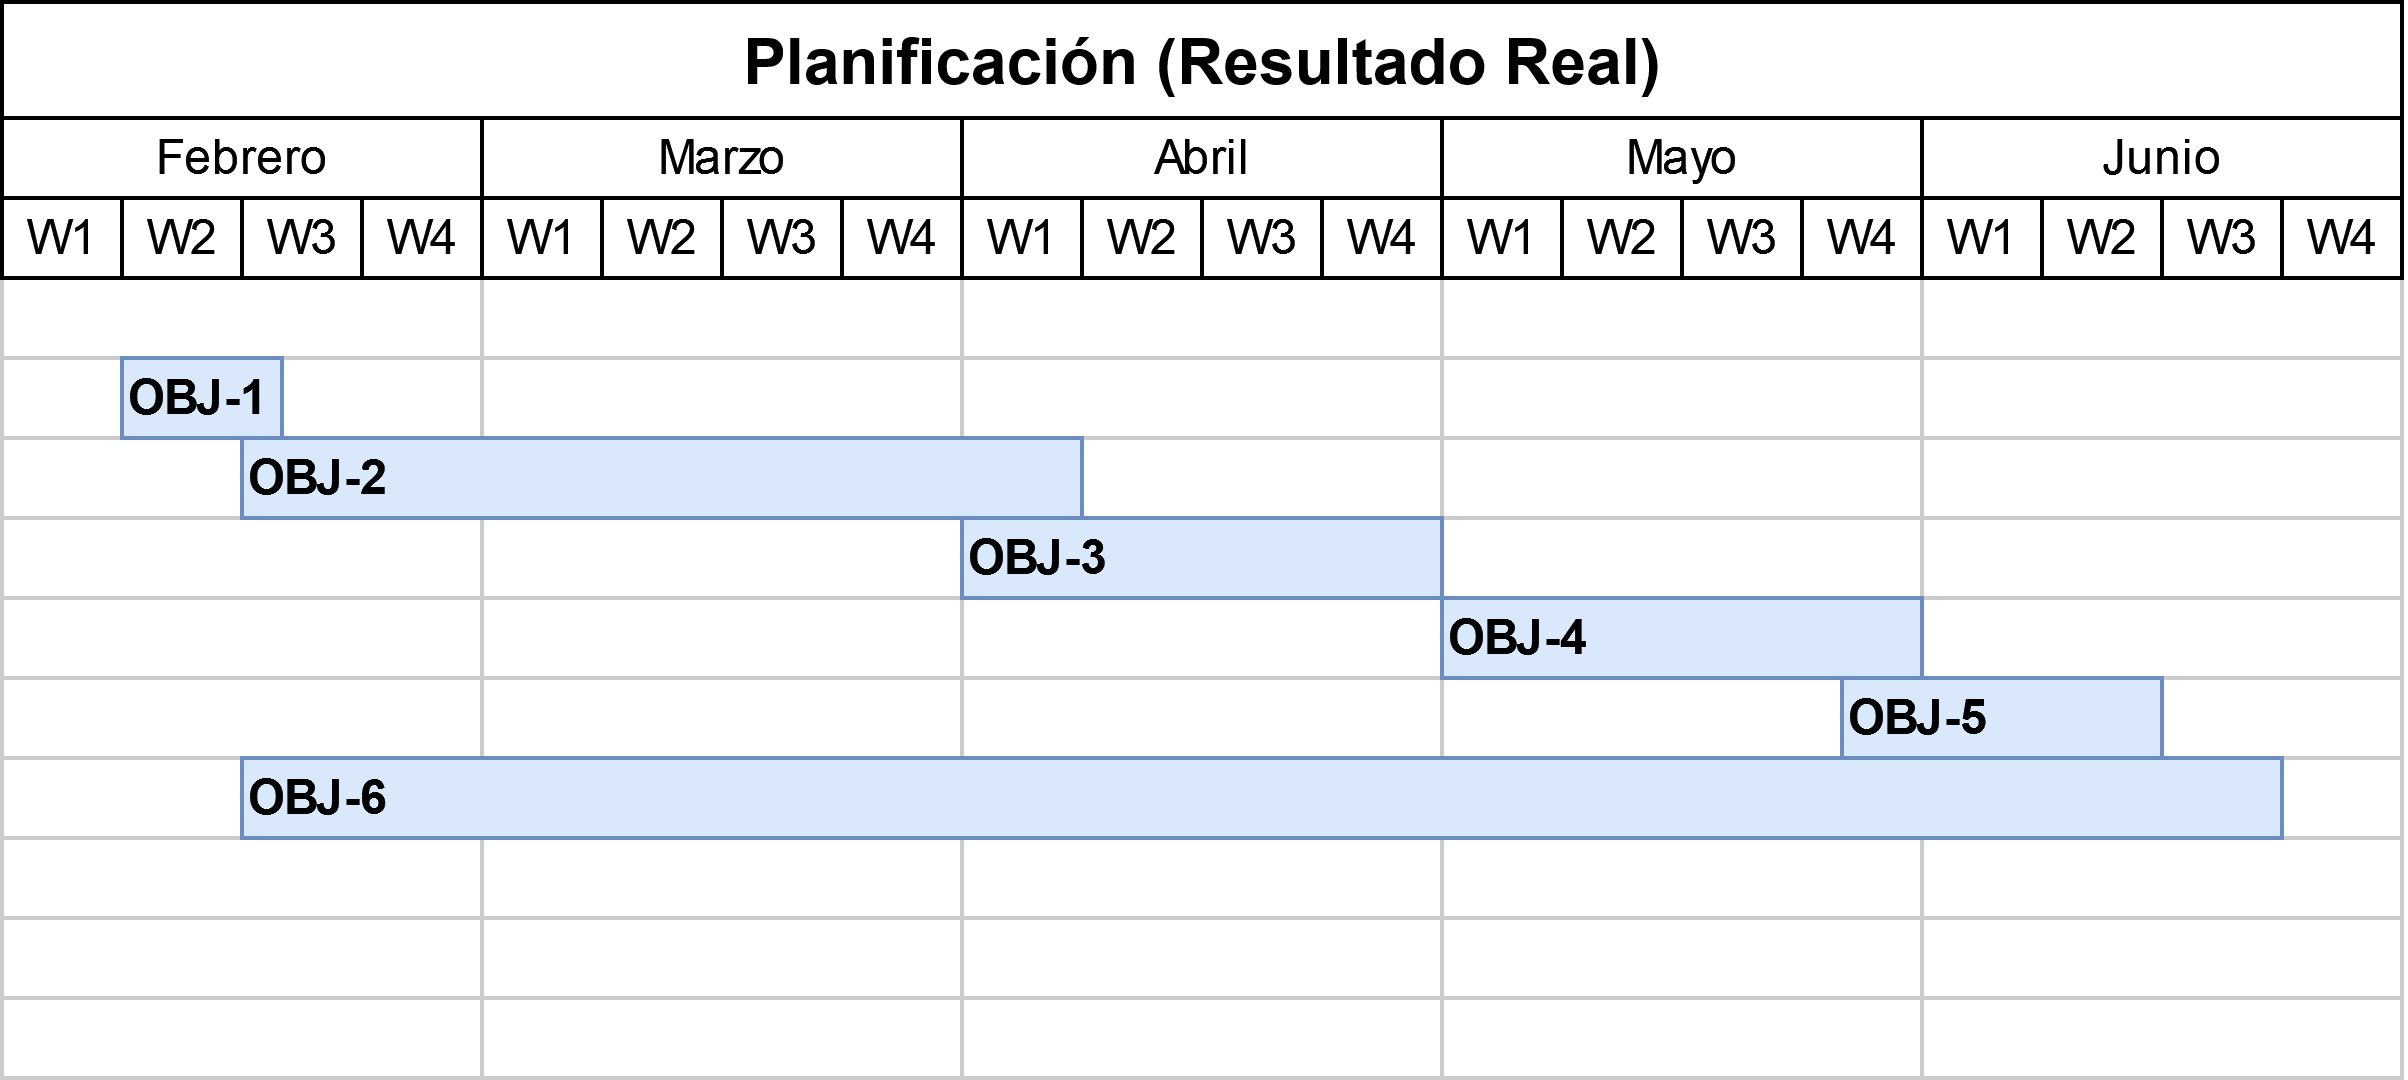
\includegraphics[width=0.99\textwidth]{img/fig/fig5.1-gantt-real.png}
    \caption{Resultados reales de la planificación}
    \label{fig:gantt-real}
\end{figure}

En general, los dos mayores cambios se realizaron en el objetivo 2 y 6 
respecto a la planificación inicial en la \autoref{fig:gantt}.
Se encontraron multitud de problemas durante el objetivo 2 que necesitaron 
mucho más tiempo del planeado, cómo fallos en el firmware de Paparazzi para el Crazyflie. 
Esto provocó un desplazamiento de los objetivos posteriores y se tuvieron que realizar un poco más deprisa.

Por otro lado, el objetivo 6 se decidió realizarse paralelamente al resto de objetivos,
es decir, se realizaban cambios y revisiones casi constantemente, así como se realizaba la memoria en paralelo con lo que se iba desarrollando. 
Esto último permitió que fuese más cómodo escribir la memoria, 
al ir plasmando lo recientemente aprendido sobre esta antes de que se olvidasen detalles en las semanas posteriores. 

%%%%%%%%%%%%%%%%%%%%%%%%%%%%%%%%%%%%%%%%%%%%%%%%%%%%%%%%%%%%%%%%%%%%%%%%%%%%%%%%%%%%%%%%%%%%%%%%%%%%%%%%%%%%%%%%%
%%%%%%%%%%%%%%%%%%%%%%%%%%%%%%%%%%%%%%%%%%%%%%%%%%%%%%%%%%%%%%%%%%%%%%%%%%%%%%%%%%%%%%%%%%%%%%%%%%%%%%%%%%%%%%%%%
%%%%%%%%%%%%%%%%%%%%%%%%%%%%%%%%%%%%%%%%%%%%%%%%%%%%%%%%%%%%%%%%%%%%%%%%%%%%%%%%%%%%%%%%%%%%%%%%%%%%%%%%%%%%%%%%%

\section{Aplicaciones y usos}

Conseguidos los fundamentos de esta tecnología de coordinación, es importante analizar las posibles aplicaciones finales.
Entre ellas, destaca principalmente la experimentación e investigación de la tecnología, 
ya que este trabajo consigue directamente esta aplicación sin mayores modificaciones y adiciones extra.

Además, la base de esta tecnología permite otros usos (por supuesto, con previas modificaciones si fuesen necesarias) 
como pueden ser la vigilancia mediante enjambres de drones, aplicaciones en agricultura, defensa o 
espectáculos de drones independientes del control por \textit{waypoints} fijados por una estación central. 

Es evidente que para terminar de ver las posibles aplicaciones y usos, 
se ha de ver que ha de mejorarse antes, por ello, lo exploraremos en la siguiente subsección.

%%%%%%%%%%%%%%%%%%%%%%%%%%%%%%%%%%%%%%%%%%%%%%%%%%%%%%%%%%%%%%%%%%%%%%%%%%%%%%%%%%%%%%%%%%%%%%%%%%%%%%%%%%%%%%%%%
%%%%%%%%%%%%%%%%%%%%%%%%%%%%%%%%%%%%%%%%%%%%%%%%%%%%%%%%%%%%%%%%%%%%%%%%%%%%%%%%%%%%%%%%%%%%%%%%%%%%%%%%%%%%%%%%%
%%%%%%%%%%%%%%%%%%%%%%%%%%%%%%%%%%%%%%%%%%%%%%%%%%%%%%%%%%%%%%%%%%%%%%%%%%%%%%%%%%%%%%%%%%%%%%%%%%%%%%%%%%%%%%%%%

\section{Trabajos y mejoras futuras}

Si se desease mejorar o continuar sobre la base de este trabajo, las primeras mejoras que se deberían aplicar serían las siguientes:

\begin{itemize}
    \item \textbf{Mejor control en Paparazzi:} al ser el primer objetivo parcialmente no cumplido, es evidente que se necesita mejor control bajo el software de Paparazzi, 
    ya que este es bastamente superado por el software oficial para los Crazyflie.

    \item \textbf{Coordinación real en Paparazzi:} consecuencia de no poder conseguir el correcto control en Paparazzi, es evidente que esto también es necesario corregirlo. 
    Es posible que consiguiendo arreglar el control no se necesite más, pero no es seguro.

    \item \textbf{Implementación para $N$ drones:} si bien el algoritmo se ha diseñado pensando en varios drones, las implementaciones se han simplificado para tan sólo dos drones. 
    Por suerte, esta mejora solo requiere cambios a la hora de introducir los parámetros de desajuste deseado y los calculos respecto a estos.

    \item \textbf{Implementación y uso de otros sistemas de posicionamiento:} 
    como bien se vio en el capítulo 1, existen más sistemas de posicionamiento compatibles con los Crazyflies.
    Estos sistemas podrían dar mayor precisión, evitar acumulación de error e incluso ayudar a la hora de implementar mejor control en Paparazzi. 
\end{itemize}

Por supuesto, esto son las mejoras directas a este TFG, si hablamos de trabajos más grandes a mayor plazo sobre esta tecnología, podemos hablar de lo siguiente:

\begin{itemize}
    \item \textbf{Implementación de GVF paramétrico:} una versión para trayectorias en tres dimensiones de GVF. Más compleja, parcialmente implementada en Paparazzi.

    \item \textbf{Mejoras diversas al software de Paparazzi:} como puede ser mayor facilidad de uso, corregir las simulaciones para el Crazyflie (aunque se pueden usar otros drones), mejorar la documentación, simplificar el software en cuestión de características (son muchas)...

    \item \textbf{Mejora general de los algoritmos:} si bien son buenos, es interesante ver hasta que punto se pueden conseguir algoritmos con mucha mayor precisión, donde el error es mínimo. También se pueden hacer algoritmos más inteligentes, que no solo sigan trayectorias semi-predefinidas.

    \item \textbf{Coordinación descentralizada y distribuida:} aplicar estos conceptos pero sin haber un nodo central, en este caso, el ordenador que controla todo. En otras palabras, coordinar $N$ drones que se comunican entre ellos y deciden que hacer sólos en base a estos algoritmos, sin un PC central que los coordine a todos.

    \item \textbf{Aplicaciones reales:} como puede ser espectáculos de luces basados en GVF, en vez de ser scripts de a que posición debe ir cada dron (como es hoy en día, generalmente).
\end{itemize}

%%%%%%%%%%%%%%%%%%%%%%%%%%%%%%%%%%%%%%%%%%%%%%%%%%%%%%%%%%%%%%%%%%%%%%%%%%%%%%%%%%%%%%%%%%%%%%%%%%%%%%%%%%%%%%%%%
%%%%%%%%%%%%%%%%%%%%%%%%%%%%%%%%%%%%%%%%%%%%%%%%%%%%%%%%%%%%%%%%%%%%%%%%%%%%%%%%%%%%%%%%%%%%%%%%%%%%%%%%%%%%%%%%%
%%%%%%%%%%%%%%%%%%%%%%%%%%%%%%%%%%%%%%%%%%%%%%%%%%%%%%%%%%%%%%%%%%%%%%%%%%%%%%%%%%%%%%%%%%%%%%%%%%%%%%%%%%%%%%%%%

\section{Conclusión}

En conclusión, este trabajo ha conseguido mayoritariamente sus objetivos, planificación y permite diversos usos. 
Se ha demostrado el buen funcionamiento de los algoritmos de estilo GVF y se han probado dos algoritmos de coordinación, uno diseñado en exclusiva para este trabajo.

Los resultados, si bien prometedores, hacen los Crazyflies ideales exclusivamente para la experimentación, investigación y educación 
en el ámbito de control y coordinación de enjambres de drones, debido a las mejoras que aún pueden añadirse, como el mejor control en Paparazzi.

Para conseguir más aplicaciones y usos, es recomendable la adición de otros componentes a este trabajo, 
como pueden ser cámaras (para vigilancia) o LEDs (para espectáculos de luces), 
así como el desarrollo extra en mejorar tanto el control como la coordinación e 
incluso avances de hardware que escapan al ámbito de este trabajo.

    \appendix

\chapter{Instalación de Paparazzi en Debian}\label{appendix:debian_install}

Paparazzi UAV solo se puede instalar oficialmente en Ubuntu \cite{paparazzi_center_install} sin realizar pasos complejos como compilación desde cero \cite{paparazzi_scratch_install}.

Desde el equipo de Swarm Systems Lab preferimos el uso de Debian a Ubuntu y, debido a su similitud,
el autor de este TFG ha descubierto un método para la instalación de Paparazzi en Debian 12, más detallado en el repositorio \cite{bt-crazyflies}.

La instalación completa se basa en ejecutar el siguiente comando en Debian. Se recomienda ejecutar el script bajo el directorio donde se desee instalar Paparazzi:

\begin{lstlisting}[style=CodigoBash]
$ wget https://raw.githubusercontent.com/Pelochus/bt-crazyflies/main/scripts/debian/paparazzi-debian-install.sh && bash paparazzi-debian-install.sh
\end{lstlisting}

En las dos siguientes secciones se explica como se instaló en detalle Paparazzi en Debian.

\section{Instalación de Paparazzi Center}

Se ha creado el siguiente script de instalación en Bash para automatizar el proceso:

\begin{lstlisting}[style=CodigoBash]
#!/bin/bash

# Needed to force a PPA repo in Debian
sudo apt install -y build-essential devscripts

# Important note: [trusted=yes] is not recommended
echo "deb [trusted=yes] https://ppa.launchpadcontent.net/paparazzi-uav/ppa/ubuntu jammy main" | sudo tee -a /etc/apt/sources.list
echo "deb-src [trusted=yes] https://ppa.launchpadcontent.net/paparazzi-uav/ppa/ubuntu jammy main" | sudo tee -a /etc/apt/sources.list

# Rest of the official Paparazzi guide
sudo apt update
sudo apt install -y paparazzi-dev gcc-arm-none-eabi gdb-multiarch python-is-python3 paparazzi-jsbsim dfu-util

# Clone Paparazzi
git clone --origin upstream https://github.com/paparazzi/paparazzi.git
cd paparazzi
git checkout v6.3 # Currently last stable version

# Compile latest stable
make
\end{lstlisting}

Para entender este script, hay que hacer hincapié en las siguientes líneas:

\begin{itemize}
    \item \textbf{Líneas 11 y 12:} Añadimos los repositorios de descarga para Paparazzi. Para que funcionen en Debian, 
    se añade \texttt{\textbf{[trusted=yes]}} de forma que se fuerce la confianza en el repositorio, ya que no es posible añadirlos de la forma natural según la guía. 
    Se indica además, que se utilice los paquetes para la última version de Ubuntu que disponen desde el equipo de Paparazzi, en este caso, \texttt{\textbf{jammy}}.

    \item \textbf{Línea 16:} Se instalan todos los paquetes según la guía oficial para Ubuntu, exceptuando el paquete para Paparazzi GCS, que no es posible utilizarlo en Debian
\end{itemize}

El resto de líneas son extraídas de la guía oficial de instalación.

Este script debe funcionar en Debian 12 recién instalado si se posee conexión a la red. 
Es posible, aunque no ha sido comprobado, que funcione en distribuciones basadas en Debian u otras versiones de Debian como Debian 11. 
No se recomienda utilizar en distribuciones basadas en Ubuntu, se puede seguir la guía oficial en estos casos.

\section{Instalación de Paparazzi GCS}
Como se ha comentado en la sección previa, el paquete correspondiente a Paparazzi GCS no se puede instalar bajo Debian.
Para ello, se puede utilizar el \textbf{AppImage} oficial, que funciona similar a un ejecutable en Windows o un contenedor de Docker.

Este AppImage necesita ser integrado con el ejecutable de Paparazzi, ya que por defecto este asume que se ha instalado 
el GCS desde el gestor de paquetes \texttt{apt} y, por tanto, hay acceso universal.

En este caso, se utiliza este script para la configuración e integración de Paparazzi GCS en Debian:

\begin{lstlisting}[style=CodigoBash]
#!/bin/bash

cd paparazzi

# Make Paparazzi GCS AppImage Work
echo "# Needed for Paparazzi AppImage to work" >> /home/$USER/.bashrc
echo "export PAPARAZZI_HOME=$(pwd)" >> /home/$USER/.bashrc
echo "export PAPARAZZI_SRC=$(pwd)" >> /home/$USER/.bashrc

# Get AppImage and move to /usr/bin/pprzgcs so it can be launched by Paparazzi Center
sudo apt install -y wget # Just in case, you should have it anyway
sudo wget https://github.com/paparazzi/PprzGCS/releases/download/v1.0.11/pprzgcs-v1.0.11-x86_64.AppImage -O /usr/bin/pprzgcs
sudo chmod 755 /usr/bin/pprzgcs
\end{lstlisting}

En este caso, es mucho más sencillo entender este script:

\begin{itemize}
    \item Primeramente se establecen las variables de entorno \texttt{PAPARAZZI\_HOME} y 
    \texttt{PAPARAZZI\_SRC}, que son necesarias para el funcionamiento del AppImage.

    \item Utilizando el ejecutable \texttt{wget}, descargamos automáticamente el AppImage y lo movemos a \texttt{/usr/bin/pprzgcs}, para que simule el comportamiento de descargar el paquete oficial de la repo. 
\end{itemize}

En general, la instalación de Paparazzi en Debian se condensa en ejecutar el primer script de este apéndice, 
que se ocupa de llamar a los otros dos scripts, de forma que se pueda modularizar la instalación de ambos componentes

\section{Instalación completa}

Para la instalación completa del código fuente de Paparazzi, 
se ejecuta el siguiente comando en el directorio raíz del repositorio:

\begin{lstlisting}[style=CodigoBash]
$ git submodule update --init --recursive .
\end{lstlisting}

Este paso no es necesario a no ser que se necesite compilar código o ejecutar simulaciones
que necesiten de código o librerías externas. 
No es necesario para el funcionamiento de Paparazzi Center y GCS.

%%%%%%%%%%%%%%%%%%%%%%%%%%%%%%%%%%%%%%%%%%%%%%%%%%%%%%%%%%%%%%%%%%%%%%%%%%%%%%%%%%%%%%%%%%%%%%%%%%%%%%%%%%%%%%%%%
%%%%%%%%%%%%%%%%%%%%%%%%%%%%%%%%%%%%%%%%%%%%%%%%%%%%%%%%%%%%%%%%%%%%%%%%%%%%%%%%%%%%%%%%%%%%%%%%%%%%%%%%%%%%%%%%%
%%%%%%%%%%%%%%%%%%%%%%%%%%%%%%%%%%%%%%%%%%%%%%%%%%%%%%%%%%%%%%%%%%%%%%%%%%%%%%%%%%%%%%%%%%%%%%%%%%%%%%%%%%%%%%%%%

% Apendice B

%%%%%%%%%%%%%%%%%%%%%%%%%%%%%%%%%%%%%%%%%%%%%%%%%%%%%%%%%%%%%%%%%%%%%%%%%%%%%%%%%%%%%%%%%%%%%%%%%%%%%%%%%%%%%%%%%
%%%%%%%%%%%%%%%%%%%%%%%%%%%%%%%%%%%%%%%%%%%%%%%%%%%%%%%%%%%%%%%%%%%%%%%%%%%%%%%%%%%%%%%%%%%%%%%%%%%%%%%%%%%%%%%%%
%%%%%%%%%%%%%%%%%%%%%%%%%%%%%%%%%%%%%%%%%%%%%%%%%%%%%%%%%%%%%%%%%%%%%%%%%%%%%%%%%%%%%%%%%%%%%%%%%%%%%%%%%%%%%%%%%

\chapter{Instalación de dependencias}\label{appendix:crazyflie_dependencies}

En el \autoref{appendix:debian_install} se incluye como se adaptó e instaló Paparazzi para Debian, no obstante,
no se incluye que librerías y configuraciones son necesarias para el uso de Crazyflie en Paparazzi.

En este segundo apartado del apéndice se incluye una breve descripción de las librerías y configuraciones necesarias. 
Se incluye aquí otro script de Bash que permite realizar todo esto de manera rápida:

\begin{lstlisting}[style=CodigoBash]
$ wget https://raw.githubusercontent.com/Pelochus/bt-crazyflies/main/scripts/deps/deps-install.sh && bash deps-install.sh
\end{lstlisting}

\section{Dependencias a instalar}
Se necesitan las siguientes dependencias:

\begin{itemize}
    \item \textbf{dfu-util y dfu-programmer:} 
    Paquetes de Ubuntu/Debian para cargar el firmware en el Crazyflie.

    \item \textbf{cflib:}
    Librería de Python para poder comunicarse con el Crazyradio 2.0 y, por tanto, un Crazyflie.

    \item \textbf{gedit:}
    Se usa por defecto para editar archivos en Paparazzi desde Paparazzi Center, al estar pensado para Ubuntu. 
    Es opcional, pero es recomendable tenerlo instalado en Debian como opción \textit{fallback}.
\end{itemize}

\section{Configuraciones y ajustes}
Por otro lado los ajustes necesarios son los siguientes:

\begin{itemize}
    \item \textbf{Añadir el usuario al grupo \texttt{dialout}:} 
    Esto sirve para poder cargar el firmware en el Crazyflie sin permisos de superusuario. 

    \item \textbf{Añadir permisos para el Crazyradio:}
    Similarmente, se añaden permisos para poder acceder al Crazyradio por USB sin ser \textit{root}. 
    Se sigue la guia oficial \cite{usb_permissions_crazyradio}.

    \item \textbf{Cambiar el editor de texto por defecto de Paparazzi Center:}
    De nuevo, opcional, pero se puede desde \textit{File - Edit settings - Text editor}
\end{itemize}

%%%%%%%%%%%%%%%%%%%%%%%%%%%%%%%%%%%%%%%%%%%%%%%%%%%%%%%%%%%%%%%%%%%%%%%%%%%%%%%%%%%%%%%%%%%%%%%%%%%%%%%%%%%%%%%%%
%%%%%%%%%%%%%%%%%%%%%%%%%%%%%%%%%%%%%%%%%%%%%%%%%%%%%%%%%%%%%%%%%%%%%%%%%%%%%%%%%%%%%%%%%%%%%%%%%%%%%%%%%%%%%%%%%
%%%%%%%%%%%%%%%%%%%%%%%%%%%%%%%%%%%%%%%%%%%%%%%%%%%%%%%%%%%%%%%%%%%%%%%%%%%%%%%%%%%%%%%%%%%%%%%%%%%%%%%%%%%%%%%%%

% Apendice C

%%%%%%%%%%%%%%%%%%%%%%%%%%%%%%%%%%%%%%%%%%%%%%%%%%%%%%%%%%%%%%%%%%%%%%%%%%%%%%%%%%%%%%%%%%%%%%%%%%%%%%%%%%%%%%%%%
%%%%%%%%%%%%%%%%%%%%%%%%%%%%%%%%%%%%%%%%%%%%%%%%%%%%%%%%%%%%%%%%%%%%%%%%%%%%%%%%%%%%%%%%%%%%%%%%%%%%%%%%%%%%%%%%%
%%%%%%%%%%%%%%%%%%%%%%%%%%%%%%%%%%%%%%%%%%%%%%%%%%%%%%%%%%%%%%%%%%%%%%%%%%%%%%%%%%%%%%%%%%%%%%%%%%%%%%%%%%%%%%%%%

\chapter{Manual de usuario}\label{appendix:user_manual}

Este manual de usuario se divide en dos partes: Paparazzi y coordinación con Bitcraze. 
Se asume que ya se puede ejecutar Paparazzi para la primera parte. 
Para la segunda, se asume que se tienen las librerías y aplicaciones de Bitcraze. 
Se puede usar la máquina virtual provista por ellos.

Si esto no es así aún, se recomienda leer los apéndices A y B o seguir las guías oficiales de instalación y configuración, 
tanto de Paparazzi como de Bitcraze, según que se vaya a utilizar.  

\section{Uso de Crazyflies en Paparazzi}

Al usar el repositorio de GitHub del autor de este TFG \cite{bt-crazyflies}, 
si se utiliza el submódulo de Paparazzi, el uso de los Crazyflies se ha simplificado
respecto al explicado en el capítulo 2 y se han añadido los pasos pertinentes para el correcto funcionamiento. Los requisitos previos son:

\begin{itemize}
    \item Se solucionaron algunos errores en el firmware. Esto ya se ha integrado en la repo de Paparazzi oficial.
    \item Se ha de cargar, previo a cargar el firmware de Paparazzi, el \textbf{firmware oficial de septiembre de 2019 (2019.09)}. 
    Si esto no es asi, no habrá correcta comunicación con la radio, ya que el firmware de la radio no es modificado por Paparazzi y este entiende a versiones antiguas.
    \item Se recomienda añadir el Flow Deck V2 mencionado en el capítulo 3, \autoref{fig:flow-deck}. Sin este, los resultados reales serán pésimos.
    \item Por último, se han añadido diversos archivos de configuración XML para facilitar un poco más el uso en Paparazzi
\end{itemize}

Para el uso de un Crazyflie, se tienen los siguientes nuevos pasos respecto al capítulo 2. Se recomienda leer el capítulo 2 para las correspondientes figuras.

\begin{itemize}
    \item En el menú desplegable arriba a la derecha, seleccionar \texttt{conf\_crazyflies.xml}
    \item En el superior izquierda, seleccionar \texttt{crazyflie-2.1} para usar el Crazyflie 2.1. 
    Se tiene soporte experimental para Crazyflie 2.0 añadido por el autor de este TFG, pero no es plenamente funcional.
    \item Para simulación, los Crazyflie no funcionan (fallo de Paparazzi), así que se recomienda seleccionar \texttt{gvf-bebop2-x},
    que tiene el mismo funcionamiento que el Crazyflie (mismos flightplan, telemetría...) pero funciona correctamente en simulación.
    \item En los dos pasos previos, por como se ha diseñado los XML, no se necesita seleccionar otros XMLs. 
    Los flightplan, airframe files, telemetry files y demás configuraciones son las correctas si no se modifican, incluyen calibraciones como las del PID.
    \item En base a si se desea simulación o real, usar uno de los dos previos y compilar \texttt{nps} para simulación o \texttt{ap} para cargar posteriormente al Crazyflie, como en el capítulo 2.
    \item Por último, dirigirse a la pestaña de \texttt{Operation} y lanzar una sesión de \texttt{Simulation} o \texttt{Crazyflie Flight} según cual se desee usar. Con esto, si se cumplen todos los pasos previos y apéndices pertinentes, debería poderse utilizar el GCS para GVF.
\end{itemize}

Finalmente, para coordinación, hay que usar los scripts que se encuentran en
\texttt{sw/ground\_segment/python/gvf} según se desee formaciones circulares o segmentos paralelos. 
Se recomienda \textbf{SÓLO USAR} para simulación, ya que la implementación real no da buenos resultados. 

La ejecución ha de realizarse tras mandar los comandos de GVF a los drones. Una vez estos esten siguiendo una trayectoria, ejecutar el script correspondiente.
Ambos scripts tienen sus menús de ayuda correspondientes para entender mejor como se ejecutan.
También se recomienda ver los ejemplos provistos en la sección 4.3 si los menús de ayuda no son suficientes.

\section{Coordinación de Crazyflies bajo firmware oficial}

Para empezar, se recomienda cargar el último firmware oficial de Bitcraze para utilizar sus herramientas \cite{crazyflie_firmware_upgrade}. 
Además, para el uso como swarm, es necesario asignar una URI distinta a cada Crazyflie mediante la configuración de este en Crazyflie Client. 
Como último requisito, se requiere el Flow Deck v2 y la Crazyradio, 
el primero para correcto movimiento y el segundo para la conexión.

Con esta base, y asumiendo la disponibilidad de las dependencias necesarias 
(estarán todas disponibles si se parte desde Bitcraze VM), 
se pueden utilizar los programas en la carpeta \texttt{python} del repositorio de este TFG \cite{bt-crazyflies}.
Alternativamente, se pueden ver los ejemplos oficiales de Bitcraze \cite{cflib-examples}

La ejecución de todos los programas que se mencionarán ahora será de la siguiente forma:

\begin{lstlisting}[style=CodigoBash]
$ python example.py
\end{lstlisting}

\subsection{Demo}

El archivo es \texttt{crazyflie\_demo.py}

Se recomienda utilizar este primer programa para asegurar el correcto funcionamiento de cada Crazyflie por separado. 
Tan sólo se debe modificar la URI del programa para que coincida con la del Crazyflie que se vaya a usar.

El programa consiste en:

\begin{itemize}
    \item Despegar el Crazyflie a 0.5 metros
    \item Moverse 0.5 metros hacia delante
    \item Volver 0.5 metros hacia atrás, tras girar 180 grados
    \item Aterrizar
\end{itemize}

\subsection{Demo para varios Crazyflies}

El archivo es \texttt{crazyflie\_swarm\_demo.py}

Similarmente al caso anterior, esto prueba que el funcionamiento en enjambre funciona.
Se debe modificar las URIs deseadas con los Crazyflies que vayan a participar.

El programa consiste en:

\begin{itemize}
    \item Parpadear los LEDs de ambos Crazyflie para asegurar que funcionan coordinadamente
    \item Despegar ambos Crazyflie a 1 metro
    \item Esperar 3 segundos
    \item Aterrizar
\end{itemize}

\subsection{Segmento para un solo Crazyflie}

El archivo es \texttt{crazyflie\_single\_segment.py}

Este programa tiene como objetivo hacer el funcionamiento de la coordinación en segmentos
pero para un solo dron, de forma que se pueda verificar que los drones se mueven correctamente a lo largo de un segmento.

Este programa consiste en:

\begin{itemize}
    \item Despegar el Crazyflie a 0.5 metros sobre el (0, 0)
    \item Moverse hasta (0.5, 0), volver hacia atras hasta la posición estimada (-0.5, 0). Las unidades son metros. Esto se hará en bucle infinito.
    \item El aterrizaje se hará tras comandar \texttt{Ctrl+C} al programa
\end{itemize}

\subsection{Coordinación en segmentos paralelos para dos Crazyflies}

El archivo es \texttt{crazyflie\_segment\_formation.py}

Este programa tiene como objetivo hacer el funcionamiento de la coordinación en segmentos que tiene este TFG como objetivo.
Se puede ampliar para funcionar con más de dos drones, pero requiere varias modificaciones. 

Este programa consiste en:

\begin{itemize}
    \item Despegar ambos Crazyflie a 0.5 metros sobre el (0, 0). 
    Cada Crazyflie en este caso, tendrán un (0, 0) distinto, se recomienda poner uno al lado del otro, separados aproximadamente medio metro.
    \item Moverse hasta (1, 0), volver hacia atras hasta la posición estimada (-1, 0). 
    Las unidades son metros. Esto se hará en bucle infinito.
    \item Mientras esto se hace, ambos Crazyflie tratarán de mantenerse uno al lado del otro.
    Por defecto, el script hará a uno de los 2 Crazyflies esperar a que el otro avance, de esta forma, tiene más sentido la coordinación. 
    Se deberá cambiar la variable \texttt{waiting\_uri} para elegir cual esperará.
    \item El aterrizaje se hará tras comandar \texttt{Ctrl+C} al programa
\end{itemize}

Si este programa funciona correctamente, deberán obtenerse resultados similares a los de este TFG.

\subsection{Coordinación en segmentos paralelos simulada}

El archivo es \texttt{sim/experiment.py}

Este programa tiene como objetivo hacer el funcionamiento de la coordinación en segmentos 
que tiene este TFG como objetivo, pero simulando uno de los dos drones.
Dado que este programa es un breve experimento, 
no esta pensado para ser usado sin previas modificaciones, añadidos o trabajos manuales.

Para usar este programa, se recomienda previamente tener un log similar al provisto en \texttt{sim/log.txt},
es decir, una sola columna con números que son las posiciones del dron real.
Alternativamente, para probar el funcionamiento se recomienda probar con el archivo provisto de ejemplo.
Se adjunta un script para convertir las comas a puntos si fuese necesario.

Para conseguir un log así se puede utilizar el programa para un solo segmento del Crazyflie explicado en este apéndice y extraer la columna de posiciones.

    \bibliography{bib/bibliografia}
    \bibliographystyle{ieeetr}
    \addcontentsline{toc}{chapter}{Bibliografia}

\end{document}